\documentclass[10pt,titlepage,english,presentation]{beamer}
\usetheme{HUB}
\setbeamercovered{invisible}
\usepackage[noborder,colbullets]{beamerMACSYdefs}

% -----------------------------------------------------------------------------
% -- packages
\usepackage{framed}
\usepackage{algorithm}
\usepackage{amsmath,amssymb,amsthm}
\usepackage{anyfontsize}
\usepackage[noend]{algpseudocode}
\algrenewcommand\alglinenumber[1]{\scriptsize #1:}
\usepackage[T1]{fontenc}
\usepackage[backend=biber,style=alphabetic,maxalphanames=1]{biblatex}
\usepackage{booktabs}
\usepackage{caption}
\usepackage{csquotes}
\usepackage{fontawesome,fourier}
\usepackage{makecell}
\usepackage{multirow}
\usepackage{numprint}
\usepackage[binary-units=true]{siunitx}
\usepackage{subcaption}
\usepackage{svg}
\usepackage[beamer,customcolors]{hf-tikz}
\usepackage{xspace}
\usefonttheme[onlymath]{serif}
\usetikzlibrary{patterns,positioning}
\usetikzlibrary{decorations.pathreplacing}
\usetikzlibrary{positioning}

\newif\ifbackup
\backuptrue

\tikzset{hl/.style={
    set fill color=red!80!black!40,
    set border color=red!80!black,
  },
}

\npthousandsep{,}
\npdecimalsign{.}

\HUBfaculty{HU Berlin}

\newcommand{\mkcolorbibparens}[2]{\textcolor{#1}{\hypersetup{citecolor=#1}{[#2]}}}
\renewenvironment{definition}[1]{\begin{block}{\vspace{-.5mm}\small Definition: #1}}{\end{block}}
\newcommand{\wmaxuv}{\ensuremath{w_{\max}(u, v)}}

\DeclareCiteCommand{\parencite}[\mkcolorbibparens{HUBblue50}]
  {\usebibmacro{prenote}}%
  {\usebibmacro{citeindex}%
   \usebibmacro{cite}}
  {\multicitedelim}
  {\usebibmacro{postnote}}

\newcommand{\speedupRoadInsBTenThou}{$\numprint{196.1}\times$\xspace}
\newcommand{\speedupRoadRemBTenThou}{$\numprint{310.4}\times$\xspace}
\newcommand{\speedupCplxInsBThou}{$\numprint{10957.5}\times$\xspace}
\newcommand{\speedupCplxRemBThou}{$\numprint{17790.7}\times$\xspace}
\newcommand{\speedupCplxInsBTenThouExp}{$\numprint{1352.5}\times$\xspace}
\newcommand{\speedupCplxInsBTenThouNorm}{$\numprint{1362.1}\times$\xspace}
\newcommand{\speedupCplxRemBTenThouExp}{$\numprint{2114.1}\times$\xspace}
\newcommand{\speedupCplxRemBTenThouNorm}{$\numprint{2135.7}\times$\xspace}
\newcommand{\speedupRMATInsBTenThou}{$\numprint{2228.7}\times$\xspace}
\newcommand{\speedupRMATRemBTenThou}{$\numprint{3719.2}\times$\xspace}
\newcommand{\speedupHYPInsBTenThou}{$\numprint{550.5}\times$\xspace}
\newcommand{\speedupHYPRemBTenThou}{$\numprint{811.6}\times$\xspace}
\newcommand{\maxAffectedInsCplx}{$\numprint{15}$\xspace}
\newcommand{\maxAffectedRemCplx}{$\numprint{13}$\xspace}
\newcommand{\maxAffectedInsRoad}{$\numprint{9}$\xspace}
\newcommand{\maxAffectedRemRoad}{$\numprint{10}$\xspace}
\newcommand{\speedBatchOverSingleRoadHundIns}{$\numprint{4.3}\times$\xspace}
\newcommand{\speedBatchOverSingleRoadHundRem}{$\numprint{5.3}\times$\xspace}
\newcommand{\speedBatchOverSingleCplxHundInsNorm}{$\numprint{7.7}\times$\xspace}
\newcommand{\speedBatchOverSingleCplxHundRemNorm}{$\numprint{10.2}\times$\xspace}
\newcommand{\speedBatchOverSingleCplxHundInsExp}{$\numprint{7.5}\times$\xspace}
\newcommand{\speedBatchOverSingleCplxHundRemExp}{$\numprint{10.7}\times$\xspace}

\newcommand{\vedgesRWInsCplxLowEps}{$\numprint{92.7}\times$\xspace}
\newcommand{\vedgesRWInsCplxHighEps}{$\numprint{34.3}\times$\xspace}
\newcommand{\vedgesRWRemCplxLowEps}{$\numprint{100.3}\times$\xspace}
\newcommand{\vedgesRWRemCplxHighEps}{$\numprint{44.3}\times$\xspace}
\newcommand{\vedgesRWInsRoadLowEps}{$\numprint{20.3}\times$\xspace}
\newcommand{\vedgesRWInsRoadHighEps}{$\numprint{8.9}\times$\xspace}
\newcommand{\vedgesRWRemRoadLowEps}{$\numprint{41.0}\times$\xspace}
\newcommand{\vedgesRWRemRoadHighEps}{$\numprint{19.8}\times$\xspace}
\newcommand{\qualRWInsCplxLowEps}{$\numprint{91.7}\%$\xspace}
\newcommand{\qualRWInsCplxHighEps}{$\numprint{93.0}\%$\xspace}
\newcommand{\qualRWRemCplxLowEps}{$\numprint{91.6}\%$\xspace}
\newcommand{\qualRWRemCplxHighEps}{$\numprint{92.9}\%$\xspace}
\newcommand{\qualRWInsRoadLowEps}{$\numprint{99.5}\%$\xspace}
\newcommand{\qualRWInsRoadHighEps}{$\numprint{99.9}\%$\xspace}
\newcommand{\qualRWRemRoadLowEps}{$\numprint{99.5}\%$\xspace}
\newcommand{\qualRWRemRoadHighEps}{$\numprint{99.9}\%$\xspace}
\newcommand{\qualDropRWInsCplxLowEps}{$\numprint{8.3}\%$\xspace}
\newcommand{\qualDropRWInsCplxHighEps}{$\numprint{7.0}\%$\xspace}
\newcommand{\qualDropRWRemCplxLowEps}{$\numprint{8.4}\%$\xspace}
\newcommand{\qualDropRWRemCplxHighEps}{$\numprint{7.1}\%$\xspace}
\newcommand{\qualDropRWInsRoadLowEps}{$\numprint{0.5}\%$\xspace}
\newcommand{\qualDropRWInsRoadHighEps}{$\numprint{0.1}\%$\xspace}
\newcommand{\qualDropRWRemRoadLowEps}{$\numprint{0.5}\%$\xspace}
\newcommand{\qualDropRWRemRoadHighEps}{$\numprint{0.1}\%$\xspace}
\newcommand{\quaRWLowest}{$\numprint{0.1}\%$\xspace}
\newcommand{\quaRWMaxDrop}{$\numprint{99.9}\%$\xspace}
\newcommand{\speedRWInsCplxLowEps}{$\numprint{1.7}\times$\xspace}
\newcommand{\speedRWInsCplxHighEps}{$\numprint{1.0}\times$\xspace}
\newcommand{\speedRWRemCplxLowEps}{$\numprint{2.9}\times$\xspace}
\newcommand{\speedRWRemCplxHighEps}{$\numprint{1.8}\times$\xspace}
\newcommand{\speedRWInsRoadLowEps}{$\numprint{3.1}\times$\xspace}
\newcommand{\speedRWInsRoadHighEps}{$\numprint{1.9}\times$\xspace}
\newcommand{\speedRWRemRoadLowEps}{$\numprint{4.5}\times$\xspace}
\newcommand{\speedRWRemRoadHighEps}{$\numprint{2.8}\times$\xspace}


\bibliography{./references.bib}

\graphicspath{{./images/}}
\newcommand{\emphcolor}{blue}
\renewcommand{\emph}[1]{\textcolor{\emphcolor}{#1}}

%%%%%%%%%%%%%%%%%%%%%%%%%%%%%%%%%%%%%%%%%%%%%%%%%%%%%%%%%%%%%%%%%%%%%%%%
% Colors
%%%%%%%%%%%%%%%%%%%%%%%%%%%%%%%%%%%%%%%%%%%%%%%%%%%%%%%%%%%%%%%%%%%%%%%%
\newcommand{\darkgreen}{black!60!green}
\newcommand{\darkorange}{brown!70!orange}

%%%%%%%%%%%%%%%%%%%%%%%%%%%%%%%%%%%%%%%%%%%%%%%%%%%%%%%%%%%%%%%%%%%%%%%%
% Chapter paragraphs
%%%%%%%%%%%%%%%%%%%%%%%%%%%%%%%%%%%%%%%%%%%%%%%%%%%%%%%%%%%%%%%%%%%%%%%%
\newcommand{\bibnotes}[1]{\paragraph{Bibliographic Notes}#1}

%%%%%%%%%%%%%%%%%%%%%%%%%%%%%%%%%%%%%%%%%%%%%%%%%%%%%%%%%%%%%%%%%%%%%%%%
% Writing
%%%%%%%%%%%%%%%%%%%%%%%%%%%%%%%%%%%%%%%%%%%%%%%%%%%%%%%%%%%%%%%%%%%%%%%%
\newcommand{\eg}{e.g.,\xspace}
\newcommand{\ie}{i.e.,\xspace}
\newcommand{\etal}{et al.\xspace}
\newcommand{\etc}{etc.\xspace}
\newcommand{\wrt}{w.r.t.\xspace} \newcommand{\aka}{a.k.a.\xspace}
\renewcommand{\th}{\textsuperscript{\textup{th}}\xspace}
\newcommand{\wilog}{w.l.o.g.\xspace}
\newcommand{\Wilog}{W.l.o.g.\xspace}
\newcommand{\np}{\ensuremath{\mathcal{NP}}}
\newcommand{\apxch}[1]{\chapter{Appendix of \Cref{#1}}}
\newcommand{\alenex}[2]{
\textit{#1 Workshop on Algorithm Engineering and Experiments (ALENEX #2)}}

%%%%%%%%%%%%%%%%%%%%%%%%%%%%%%%%%%%%%%%%%%%%%%%%%%%%%%%%%%%%%%%%%%%%%%%%
% Math
%%%%%%%%%%%%%%%%%%%%%%%%%%%%%%%%%%%%%%%%%%%%%%%%%%%%%%%%%%%%%%%%%%%%%%%%
\newcommand{\set}[1]{\ensuremath{\left\lbrace#1\right\rbrace}}
\renewcommand{\iff}{\ensuremath{\Leftrightarrow}}
\newcommand{\Oh}{\ensuremath{\mathcal{O}}}
\newcommand{\fdist}{\ensuremath{\zeta}}
\newcommand{\fdistp}{\ensuremath{\fdist_{\alpha}}}
\newcommand{\ct}{\ensuremath{t_c}}
\newcommand{\ctg}{\ensuremath{t_{c, G}}}
\newcommand{\hitt}{\ensuremath{t_h}}
\newcommand{\expected}[1]{\ensuremath{\mathbf{E}\left[#1\right]}}
\DeclareMathOperator{\gmean}{GM}
\DeclareMathOperator*{\argmax}{argmax}
\DeclareMathOperator*{\argmin}{argmin}
\newcommand{\norm}[1]{\left\lVert#1\right\rVert}
\newcommand{\onenorm}[1]{\left\lVert#1\right\rVert_1}
\newcommand{\twonorm}[1]{\left\lVert#1\right\rVert_2}
\newcommand{\maxnorm}[1]{\left\lVert#1\right\rVert_{\infty}}
\newcommand{\natn}{\ensuremath{\mathbb{N}}}
\newcommand{\ratn}{\ensuremath{\mathbb{Q}}}
\newcommand{\pair}[2]{\ensuremath{\left<#1, #2\right>}}
\newcommand{\poly}{\text{poly}}
\newcommand{\lonerel}{\ensuremath{\mathrm{L1}_\mathrm{rel}}}
\newcommand{\ltworel}{\ensuremath{\mathrm{L2}_\mathrm{rel}}}
\newcommand{\erel}{\ensuremath{\mathrm{E}_\mathrm{rel}}}

\renewcommand{\epsilon}{\varepsilon}

%%%%%%%%%%%%%%%%%%%%%%%%%%%%%%%%%%%%%%%%%%%%%%%%%%%%%%%%%%%%%%%%%%%%%%%%
% Graph Measures
%%%%%%%%%%%%%%%%%%%%%%%%%%%%%%%%%%%%%%%%%%%%%%%%%%%%%%%%%%%%%%%%%%%%%%%%
\newcommand{\vol}{\ensuremath{\text{vol}}}
\newcommand{\nout}{\ensuremath{N_{\text{out}}}}
\newcommand{\nin}{\ensuremath{N_{\text{in}}}}
\newcommand{\degin}{\ensuremath{\deg_{\text{in}}}}
\newcommand{\degout}{\ensuremath{\deg_{\text{out}}}}
\newcommand{\diam}{\ensuremath{\text{diam}}}
\newcommand{\ecc}{\ensuremath{\text{ecc}}}
\newcommand{\kidx}{\ensuremath{\mathcal{K}}}

%%%%%%%%%%%%%%%%%%%%%%%%%%%%%%%%%%%%%%%%%%%%%%%%%%%%%%%%%%%%%%%%%%%%%%%%
% Formatting numbers
%%%%%%%%%%%%%%%%%%%%%%%%%%%%%%%%%%%%%%%%%%%%%%%%%%%%%%%%%%%%%%%%%%%%%%%%
\newcommand{\onedigit}[1]{
\ensuremath{\num[round-mode=places,round-precision=1]{#1}}
}

%%%%%%%%%%%%%%%%%%%%%%%%%%%%%%%%%%%%%%%%%%%%%%%%%%%%%%%%%%%%%%%%%%%%%%%%
% Parentheses
%%%%%%%%%%%%%%%%%%%%%%%%%%%%%%%%%%%%%%%%%%%%%%%%%%%%%%%%%%%%%%%%%%%%%%%%
\newcommand{\roundb}[1]{\ensuremath{\left(#1\right)}}
\newcommand{\ceil}[1]{\ensuremath{\left\lceil#1\right\rceil}}

%%%%%%%%%%%%%%%%%%%%%%%%%%%%%%%%%%%%%%%%%%%%%%%%%%%%%%%%%%%%%%%%%%%%%%%%
% Matrices and Vectors
%%%%%%%%%%%%%%%%%%%%%%%%%%%%%%%%%%%%%%%%%%%%%%%%%%%%%%%%%%%%%%%%%%%%%%%%
\newcommand{\mat}[1]{\ensuremath{\mathbf{#1}}\xspace}
\newcommand{\vect}[1]{\ensuremath{\mathbf{#1}}\xspace}
\newcommand{\Adj}{\mat{A}}
\newcommand{\Deg}{\mat{D}}
\newcommand{\Ones}{\mat{J}}
\newcommand{\ones}{\mat{j}}
\newcommand{\Ident}{\mat{I}}
\newcommand{\Fmat}{\ensuremath{\bm{\Omega}}\xspace}
\newcommand{\Fmatapx}{\ensuremath{\widetilde{\Fmat}}\xspace}
\newcommand{\Fmatp}{\ensuremath{\bm{\Omega}_{\alpha}}\xspace}
\newcommand{\cunit}[1]{\ensuremath{\vect{e}_{#1}}}
\newcommand{\diag}[1]{\ensuremath{\text{diag}\roundb{#1}}\xspace}
\newcommand{\tr}[1]{\ensuremath{\text{tr}\roundb{#1}}\xspace}
\newcommand{\xapprox}{\ensuremath{\widetilde{\vect{x}}}}

%%%%%%%%%%%%%%%%%%%%%%%%%%%%%%%%%%%%%%%%%%%%%%%%%%%%%%%%%%%%%%%%%%%%%%%%
% Effective Resistance Notation
%%%%%%%%%%%%%%%%%%%%%%%%%%%%%%%%%%%%%%%%%%%%%%%%%%%%%%%%%%%%%%%%%%%%%%%%
\newcommand{\reff}{\ensuremath{r_{\text{eff}}}\xspace}
\newcommand{\ceff}{\ensuremath{c_{\text{eff}}}\xspace}
\newcommand{\rdist}{\ensuremath{\rho}\xspace}
\newcommand{\rdistapx}{\ensuremath{\tilde{\rho}}\xspace}
\newcommand{\rdiststar}{\ensuremath{\rho_{\star}}\xspace}
\newcommand{\rdiststarapx}{\ensuremath{\tilde{\rho}_{\star}}\xspace}
\newcommand{\Lapl}{\mat{L}}
\newcommand{\Lstar}{\mat{L_{\star}}}
\newcommand{\Linv}{\ensuremath{\Lapl^\dagger}\xspace}
\newcommand{\Linvstar}{\ensuremath{\Lapl^\dagger_\star}\xspace}
\newcommand{\Linvapx}{\ensuremath{\widetilde{\Lapl^\dagger}}\xspace}

%%%%%%%%%%%%%%%%%%%%%%%%%%%%%%%%%%%%%%%%%%%%%%%%%%%%%%%%%%%%%%%%%%%%%%%%
% Centrality Measures
%%%%%%%%%%%%%%%%%%%%%%%%%%%%%%%%%%%%%%%%%%%%%%%%%%%%%%%%%%%%%%%%%%%%%%%%
\newcommand{\clos}{\ensuremath{c_c}\xspace}
\newcommand{\farn}{\ensuremath{f}\xspace}
\newcommand{\elfarn}{\ensuremath{f_e}\xspace}
\newcommand{\ffarnp}{\ensuremath{f_{f, \alpha}}\xspace}
\newcommand{\ffarn}{\ensuremath{f_f}\xspace}
\newcommand{\harm}{\ensuremath{c_h}}
\newcommand{\harmupp}{\ensuremath{\widetilde{\harm}}}
\newcommand{\betw}{\ensuremath{c_b}\xspace}
\newcommand{\bapx}{\ensuremath{\tilde{c}_b}\xspace}
\newcommand{\nrwb}{\ensuremath{c_{\text{nrwb}}}\xspace}
\newcommand{\katz}{\ensuremath{c_{\text{K}}}}
\newcommand{\edw}{ED-Walk\xspace}
\newcommand{\ed}{\ensuremath{c_{\text{ED}}}}
\newcommand{\eig}{\ensuremath{c_{\text{eig}}}}
\newcommand{\pr}{\ensuremath{c_{\text{PR}}}}
\newcommand{\elclos}{\ensuremath{c_e}}
\newcommand{\fclos}{\ensuremath{c_f}}
\newcommand{\fclosp}{\ensuremath{c_{f,\alpha}}}

\newcommand{\gdeg}{\ensuremath{g_d}\xspace}
\newcommand{\gclos}{\ensuremath{g_c}\xspace}
\newcommand{\gfarn}{\ensuremath{g_f}\xspace}
\newcommand{\gffarn}{\ensuremath{g_{\mathit{ff}}\xspace}}
\newcommand{\gffarnp}{\ensuremath{g_{\mathit{ff},\alpha}\xspace}}
\newcommand{\gharm}{\ensuremath{g_h}\xspace}
\newcommand{\gfclos}{\ensuremath{g_{\mathit{fc}}}\xspace}
\newcommand{\gfclosp}{\ensuremath{g_{\mathit{fc},\alpha}}\xspace}
\newcommand{\gharmupp}{\ensuremath{\widehat{\gharm}}\xspace}
\newcommand{\gfarnapx}{\ensuremath{\widetilde{\gfarn}}\xspace}
\newcommand{\gfarnupp}{\ensuremath{\widehat{\gfarn}}\xspace}
\newcommand{\ged}{\ensuremath{g_{\text{ED}}}}
\newcommand{\gedll}{\ensuremath{g_{\text{ED}}^{\le\ell}}}
\newcommand{\gedgl}{\ensuremath{g_{\text{ED}}^{>\ell}}}

%%%%%%%%%%%%%%%%%%%%%%%%%%%%%%%%%%%%%%%%%%%%%%%%%%%%%%%%%%%%%%%%%%%%%%%%
% Specific Notations
%%%%%%%%%%%%%%%%%%%%%%%%%%%%%%%%%%%%%%%%%%%%%%%%%%%%%%%%%%%%%%%%%%%%%%%%
\newcommand{\dcut}{\ensuremath{d_{\text{cut}}}}
\newcommand{\isexact}{\texttt{isExact}\xspace}
\newcommand{\imax}{\ensuremath{i_{\max}}\xspace}
\newcommand{\Suv}{\ensuremath{S_{-u}^{+v}}}
\newcommand{\Su}{\ensuremath{S_{-u}}}
\newcommand{\Sv}{\ensuremath{S^{+v}}}
\newcommand{\deltafarnm}{\ensuremath{\Delta^-}}
\newcommand{\deltafarnp}{\ensuremath{\Delta^+}}
\newcommand{\Huvp}{\ensuremath{H_{u, v}^+}}
\newcommand{\Huvm}{\ensuremath{H_{u, v}^-}}
\newcommand{\Luvo}{\ensuremath{L_{u, v}^0}}
\newcommand{\Huvo}{\ensuremath{H_{u, v}^0}}
\newcommand{\wmin}{\ensuremath{w_{\min}}}
\newcommand{\wmax}{\ensuremath{w_{\max}}}
\newcommand{\PhiSu}{\ensuremath{\Phi_{S, u}}}
\newcommand{\PhiSv}{\ensuremath{\Phi_{S, v}}}
\newcommand{\phit}{\ensuremath{\phi^{\text{hit}}}}
\newcommand{\pmiss}{\ensuremath{\phi^{\text{miss}}}}
\newcommand{\pshit}{\ensuremath{\psi^{\text{hit}}}}
\newcommand{\psmiss}{\ensuremath{\psi^{\text{miss}}}}
\newcommand{\degmax}{\ensuremath{\deg_{\max}}}
\newcommand{\erdosr}{Erd\H{o}s R\'enyi\xspace}
\newcommand{\interm}{\ensuremath{^{(i)}}\xspace}
\newcommand{\iinterm}{\ensuremath{^{(ii)}}\xspace}
\newcommand{\final}{\ensuremath{^{(f)}}\xspace}
\newcommand{\iteri}{^{[i]}}
\newcommand{\iter}[1]{^{[#1]}}

\newcommand{\tdis}{\ensuremath{t_{\text{dis}}}}
\newcommand{\tfin}{\ensuremath{t_{\text{fin}}}}
\newcommand{\gstar}{\ensuremath{G_{\star}}\xspace}
\newcommand{\gstarp}{\ensuremath{G_{\star,\alpha}}\xspace}

\newcommand{\graphfh}{edge factor 16, $a = \numprint{0.57}, b =
\numprint{0.19}, c = \numprint{0.19},$ and $d = \numprint{0.05}$\xspace}

\DeclareMathOperator{\rlxmove}{\gets_\mathsf{relaxed}}
\DeclareMathOperator{\loadacq}{\gets_\mathsf{acquire}}
\DeclareMathOperator{\storerel}{\gets_\mathsf{release}}

%%%%%%%%%%%%%%%%%%%%%%%%%%%%%%%%%%%%%%%%%%%%%%%%%%%%%%%%%%%%%%%%%%%%%%%%
% Tools
%%%%%%%%%%%%%%%%%%%%%%%%%%%%%%%%%%%%%%%%%%%%%%%%%%%%%%%%%%%%%%%%%%%%%%%%
\newcommand{\nwkurl}{\url{https://github.com/networkit/networkit/}\xspace}

%%%%%%%%%%%%%%%%%%%%%%%%%%%%%%%%%%%%%%%%%%%%%%%%%%%%%%%%%%%%%%%%%%%%%%%%
% Tikz
%%%%%%%%%%%%%%%%%%%%%%%%%%%%%%%%%%%%%%%%%%%%%%%%%%%%%%%%%%%%%%%%%%%%%%%%
\newcommand{\vertex}[2]{\node[minimum size=5mm,circle,draw] (#2) at (#1) {#2};}
\newcommand{\filledvertex}[1]{\draw[fill] (#1) circle [radius=2pt];}
\newcommand{\edge}[2]{\draw[-] (#1) -- (#2);}
\newcommand{\myarrow}{\draw[-{latex[scale=2]}]}
\newcommand{\myarrowcolor}[1]{\draw[-{latex[scale=2]},#1]}
\newcommand{\mydoublearrow}{\draw[latex'-latex']}
\newcommand{\dedge}[2]{\myarrow (#1) -- (#2);}
\newcommand{\dedgecolor}[3]{\myarrowcolor{#3} (#1) -- (#2);}
\newcommand{\dbedge}[3]{\myarrow (#1) edge [#3] node {} (#2);}
\newcommand{\ddedge}[2]{\mydoublearrow (#1) -- (#2);}
\newcommand{\thickedge}[2]{\draw[-, line width=.4mm] (#1) -- (#2);}
\newcommand{\dashedEdge}[2]{\draw[dashed] (#1) -- (#2);}
\newcommand{\dottedEdge}[2]{\draw[dotted] (#1) -- (#2);}
\newcommand{\dashdottedEdge}[2]{\draw[dash dot] (#1) -- (#2);}
\newcommand{\eqnode}[2]{
\node[] at (#1){\begin{minipage}{\textwidth}#2\end{minipage}};
}
\tikzstyle{graphnode}=[circle,draw,thick]
\tikzstyle{groupstyle}=[dashed, thick]
\newcommand{\simplenode}[2]{\node[graphnode] (#1) at (#2) {};}
\newcommand{\colornode}[2]{\node[graphnode, \darkorange] (#1) at (#2) {};}
\newcommand{\customcolornode}[3]{\node[graphnode,fill, #3,thick,draw=black] (#1) at (#2) {};}
\newcommand{\colortextnode}[3]{\node[graphnode, \darkorange] (#1) at (#2) {#3};}
\newcommand{\textnode}[3]{\node[graphnode, minimum size=4mm] (#1) at (#2) {#3};}
\newcommand{\textnodecolor}[4]{\node[graphnode, minimum size=4mm,fill,#4] (#1) at (#2) {#3};}
\newcommand{\nshift}{5pt}

%%%%%%%%%%%%%%%%%%%%%%%%%%%%%%%%%%%%%%%%%%%%%%%%%%%%%%%%%%%%%%%%%%%%%%%%
% Functions and Algorithms
%%%%%%%%%%%%%%%%%%%%%%%%%%%%%%%%%%%%%%%%%%%%%%%%%%%%%%%%%%%%%%%%%%%%%%%%
\newcommand{\func}[1]{\textsf{#1}\xspace}
\newcommand{\nbcut}{\func{NBCut}}
\newcommand{\bfscut}{\func{BFScut}}
\newcommand{\nbbound}{\func{NBBound}}
\newcommand{\bfsbound}{\func{BFSbound}}
\newcommand{\localswaps}{\textit{Local-Swaps}\xspace}
\newcommand{\growshrink}{\textit{Grow-Shrink}\xspace}
\newcommand{\greedyh}{\func{Greedy-H}}
\newcommand{\greedylsh}{\func{Greedy-LS-H}}
\newcommand{\bestrandomh}{\func{Best-Random-H}}
\newcommand{\greedyc}{\func{Greedy-C}}
\newcommand{\gs}{\func{GS}}
\newcommand{\bestrandomc}{\func{Best-Random-C}}
\newcommand{\greedylsc}{\func{Greedy-LS-C}}
\newcommand{\gslsc}{\func{GS-LS-C}}
\newcommand{\ust}{\func{UST}}
\newcommand{\lamgjlt}{\func{Lamg-jlt}}
\newcommand{\juliajlt}{\func{Julia-jlt}}
\newcommand{\jltjulia}{\func{JLT-Julia}}
\newcommand{\jltcpp}{\func{JLT-CPP}}
\newcommand{\bekas}{\func{Bekas}}
\newcommand{\bekash}{\func{Bekas-h}}
\newcommand{\suitor}{\func{Suitor}}
\newcommand{\dynmwmrandom}{\func{DynMWMRandom}}
\newcommand{\ssuitor}{\func{SortSuitor}}
\newcommand{\findsuitor}{\func{findSuitor}}
\newcommand{\findaff}{\func{findAffected}}
\newcommand{\findaffb}{$\func{findAffected}_B$\xspace}
\newcommand{\updateaff}{\func{updateAffected}}
\newcommand{\affected}{\ensuremath{\mathit{affected}}\xspace}
\newcommand{\heaviest}{\ensuremath{\mathit{heaviest}}\xspace}
\newcommand{\partner}{\ensuremath{\mathit{partner}}\xspace}
\newcommand{\done}{\ensuremath{\mathit{done}}\xspace}
\newcommand{\vsuitor}{\ensuremath{\mathit{suitor}}\xspace}
\newcommand{\cur}{\ensuremath{\mathit{cur}}\xspace}
\newcommand{\mate}{\ensuremath{\mathit{mate}}\xspace}
\newcommand{\nextCand}{\texttt{nextCandidate}\xspace}

\newcommand{\localframe}{\textit{local-frame}\xspace}
\newcommand{\Localframe}{\textit{Local-frame}\xspace}
\newcommand{\sharedframe}{\textit{shared-frame}\xspace}
\newcommand{\Sharedframe}{\textit{Shared-frame}\xspace}
\newcommand{\indexedframe}{\textit{indexed-frame}\xspace}
\newcommand{\Indexedframe}{\textit{Indexed-frame}\xspace}
\newcommand{\kadabra}{\func{KADABRA}}
\newcommand{\rk}{\func{RK}}

%%%%%%%%%%%%%%%%%%%%%%%%%%%%%%%%%%%%%%%%%%%%%%%%%%%%%%%%%%%%%%%%%%%%%%%%
% Pseudocode
%%%%%%%%%%%%%%%%%%%%%%%%%%%%%%%%%%%%%%%%%%%%%%%%%%%%%%%%%%%%%%%%%%%%%%%%
\newcommand{\topk}{\texttt{TopK}\xspace}
\newcommand{\prioq}{\texttt{PrioQ}\xspace}
\newcommand{\true}{\texttt{true}\xspace}
\newcommand{\false}{\texttt{false}\xspace}
\newcommand{\nil}{\texttt{null}\xspace}
\newcommand{\didswap}{\texttt{didSwap}\xspace}
\newcommand{\TopComment}[1]{\State\texttt{/* #1 */}}

%%%%%%%%%%%%%%%%%%%%%%%%%%%%%%%%%%%%%%%%%%%%%%%%%%%%%%%%%%%%%%%%%%%%%%%%
% Cluster specs
%%%%%%%%%%%%%%%%%%%%%%%%%%%%%%%%%%%%%%%%%%%%%%%%%%%%%%%%%%%%%%%%%%%%%%%%
\newcommand{\RAM}{$\SI{192}{\gibi\byte}$ of RAM\xspace}
\newcommand{\cpumodel}{Intel Xeon Gold 6126\xspace}
\newcommand{\CPU}{\cpumodel with $2\times12$ cores\xspace}
\newcommand{\egocpu}{Intel Xeon Gold 6154\xspace}
\newcommand{\egoram}{$\SI{1.5}{\tebi\byte}$ of RAM\xspace}

%%%%%%%%%%%%%%%%%%%%%%%%%%%%%%%%%%%%%%%%%%%%%%%%%%%%%%%%%%%%%%%%%%%%%%%%
% Changed text after first submission
%%%%%%%%%%%%%%%%%%%%%%%%%%%%%%%%%%%%%%%%%%%%%%%%%%%%%%%%%%%%%%%%%%%%%%%%
\newif\ifchanges
\newcommand{\change}[1]{\ifchanges\textcolor{blue}{#1}\else#1\fi}

\newcommand{\swapMaxSpeed}{1445.0232496265153}
\newcommand{\swapMinSpeed}{86.9541039632718}
\newcommand{\swapMaxvMinQual}{77.8881228997525}
\newcommand{\swapMaxvMaxQual}{83.29810184779429}
\newcommand{\swapMaxvKQual}{81.40970843352184}
\newcommand{\swapMaxvKSpeed}{1445.0232496265153}
\newcommand{\swapMaxQualityDrop}{22.1118771002475}
\newcommand{\gsMaxSpeed}{927.871445138909}
\newcommand{\gsMinSpeed}{42.96954466604031}
\newcommand{\gsMinQual}{88.97660094864452}
\newcommand{\gsMaxQual}{99.6012068106976}
\newcommand{\gsLocalMinQual}{8.112812959119452}
\newcommand{\gsLocalMaxQual}{7.096158766270122}
\newcommand{\gsLocalMinSpeed}{81.33565413999767}
\newcommand{\gsLocalMaxSpeed}{512.3211951631533}
\newcommand{\gsInsMinQual}{91.88718704088055}
\newcommand{\gsInsMaxQual}{98.50660111050259}
\newcommand{\gsExpMinQual}{94.82151212051194}
\newcommand{\gsExpMaxQual}{99.6012068106976}
\newcommand{\swapKQual}{78.95512599304074}
\newcommand{\gsPKQual}{0.9497061887060232}
\newcommand{\gsPKQualNum}{99.05029381129398}
\newcommand{\gsPKSpeed}{134.37637156954395}
\newcommand{\gsPSevenFiveKQualNum}{99.38257368840114}
\newcommand{\gsPSevenFiveKSpeed}{127.83319715440305}
\newcommand{\maxQual}{99.6012068106976}
\newcommand{\minQualDrop}{0.39879318930239327}
\newcommand{\swapMinQualDrop}{10.452777368923183}
\newcommand{\minSpeedupKHundred}{42.96954466604031}
\newcommand{\gsLocalSpeedupOverNonLocal}{3.1341149912690742}
\newcommand{\gsLocalSpeedKTen}{365.83696556394904}
\newcommand{\gsLocalQualKTen}{92.0747944022351}
\newcommand{\wGSQualInc}{12.384054953251923}
\newcommand{\wGSSpeed}{793.6424400458743}

\newcommand{\grayedonslide}[3]{
\only<#1>{#3}
\only<#2>{#3}
}

\newcommand{\coorda}{2.7, 0}
\newcommand{\nodeida}{s1}

\newcommand{\coordb}{2.5, 1}
\newcommand{\nodeidb}{s2}

\newcommand{\coordc}{2.5, -1}
\newcommand{\nodeidc}{s3}

\newcommand{\coordd}{2, -1.6}
\newcommand{\nodeidd}{s4}

\newcommand{\coorde}{1, 0}
\newcommand{\nodeide}{s5}

\newcommand{\coordf}{.75, .6}
\newcommand{\nodeidf}{s6}

\newcommand{\coordg}{3, -2.2}
\newcommand{\nodeidg}{n1}

\newcommand{\coordh}{3.8, -0.8}
\newcommand{\nodeidh}{n2}

\newcommand{\coordi}{3.7, 0}
\newcommand{\nodeidi}{n3}

\newcommand{\coordj}{3.5, 0.7}
\newcommand{\nodeidj}{n4}

\newcommand{\coordk}{5, -2.1}
\newcommand{\nodeidk}{n5}

\newcommand{\coordl}{5.1, -1.5}
\newcommand{\nodeidl}{n6}

\newcommand{\coordm}{5.9, -0.8}
\newcommand{\nodeidm}{n7}

\newcommand{\coordn}{5.7, 0}
\newcommand{\nodeidn}{n8}

\newcommand{\coordo}{5.5, 1}
\newcommand{\nodeido}{n9}

\newcommand{\coordp}{7.5, -1.2}
\newcommand{\nodeidp}{n10}

\newcommand{\coordq}{7.7, 0}
\newcommand{\nodeidq}{n11}

\newcommand{\coordr}{7, 0.7}
\newcommand{\nodeidr}{n12}

\newcommand{\edgecoords}{
\path (s1) ++(0:\nshift) coordinate (sg1);
\path (s1) ++(-30:\nshift) coordinate (sg11);
\path (s1) ++(90:\nshift) coordinate (sg12);
\path (s1) ++(0:\nshift) coordinate (sg1);
\path (s2) ++(-20:\nshift) coordinate (sg2);
\path (s2) ++(180:\nshift) coordinate (sg2b);
\path (s2) ++(270:\nshift) coordinate (sg2bb);
\path (s3) ++(0:\nshift) coordinate (sg3);
\path (s3) ++(150:\nshift) coordinate (sg3b);
\path (s4) ++(-30:\nshift) coordinate (sg4);
\path (s5) ++(-30:\nshift) coordinate (sg5);
\path (s6) ++(15:\nshift) coordinate (sg6);

\path (n1) ++(150:\nshift) coordinate (ng1);
\path (n2) ++(180:\nshift) coordinate (ng2);
\path (n2) ++(150:\nshift) coordinate (ng21);
\path (n3) ++(180:\nshift) coordinate (ng3);
\path (n4) ++(165:\nshift) coordinate (ng4);
\path (n1) ++(0:\nshift) coordinate (ng1b);
\path (n2) ++(0:\nshift) coordinate (ng2b);
\path (n2) ++(30:\nshift) coordinate (ng2b1);
\path (n2) ++(-30:\nshift) coordinate (ng2b2);
\path (n3) ++(0:\nshift) coordinate (ng3b);
\path (n3) ++(30:\nshift) coordinate (ng3b1);

\path (n5) ++(180:\nshift) coordinate (ng5);
\path (n6) ++(150:\nshift) coordinate (ng6);
\path (n7) ++(180:\nshift) coordinate (ng7);
\path (n8) ++(180:\nshift) coordinate (ng8);
\path (n8) ++(210:\nshift) coordinate (ng81);
\path (n9) ++(210:\nshift) coordinate (ng9);

\path (n7) ++(-10:\nshift) coordinate (ng6b);
\path (n8) ++(0:\nshift) coordinate (ng7b);
\path (n8) ++(30:\nshift) coordinate (ng7b1);
\path (n9) ++(0:\nshift) coordinate (ng8b);

\path (n10) ++(160:\nshift) coordinate (ng10);
\path (n11) ++(180:\nshift) coordinate (ng11);
\path (n12) ++(210:\nshift) coordinate (ng12);
}

\tikzstyle{groupstyle}=[dashed, thick]
\tikzstyle{graphnode}=[circle,draw,thick]
\tikzstyle{every node}=[font=\small\itshape,inner sep=0, minimum size=.25cm, outer sep=0]

\newcommand{\grouplegend}{
\node[align=right] at (-1.25, .25) {$S$};
\draw[groupstyle,black] (-.75, .25) to (-.25, .25);
}
\newcommand{\graphlegend}{
\grouplegend
\node[align=right] at (-1.25, -.25) {\textnormal{DAG}};
\draw[black] (-.75, -.25) to (-.25, -.25);
}

\newcommand{\graphcoords}{
\coordinate[] (g1) at (0, 0);
\coordinate[] (g2) at (2, -2);
\coordinate[] (g3) at (4, -3);
\coordinate[] (g4) at (6, -2);
\coordinate[] (g5) at (8, -1);
\coordinate[] (g6) at (9, 0);
\coordinate[] (g7) at (7, 1);
\coordinate[] (g8) at (3, 1.2);
}

\newcommand{\graphcontour}{
\draw[] (g1) to[out=-90,in=180] (g2);
\draw[] (g2) to[out=0,in=180] (g3);
\draw[] (g2) to[out=0,in=180] (g3);
\draw[] (g3) to[out=0,in=200] (g4);
\draw[] (g4) to[out=30,in=240] (g5);
\draw[] (g5) to[out=60,in=-90] (g6);
\draw[] (g6) to[out=90,in=-30] (g7);
\draw[] (g7) to[out=150,in=-20] (g8);
\draw[] (g8) to[out=150,in=90] (g1);
}

\newcommand{\drawgraphcontour}{
\graphlegend
\graphcoords
\graphcontour
}

\newcommand{\drawgroupcontour}{
\coordinate[] (s1) at (3, 0);
\coordinate[] (s2) at (2, 0);
\coordinate[] (s4) at (2.5, 1.3);
\draw[dashed, thick] (s2) to[out=-90,in=180] ([yshift=5pt]g2);
\draw[dashed, thick] ([yshift=5pt]g2) to[out=0,in=-90] (s1);
\draw[dashed, thick] (s1) to[out=90,in=0] (s4);
\draw[dashed, thick] (s4) to[out=180,in=90] (s2);
}

\newcommand{\drawgroupsemilocaladdcontour}{
\coordinate[] (s1) at (4, -1);
\coordinate[] (s11) at (4, -.5);
\coordinate[] (s12) at (3, 0);
\coordinate[] (s2) at (2, 0);
\coordinate[] (s3) at (2.75, 1);
\coordinate[] (s4) at (2.25, 1.3);
\draw[dashed, thick] (s2) to[out=-90,in=180] ([yshift=5pt]g2);
\draw[dashed, thick] ([yshift=5pt]g2) to[out=0,in=-90] (s1);
\draw[dashed, thick] (s1) to[out=90,in=-90] (s11);
\draw[dashed, thick] (s11) to[out=120,in=-90] (s12);
\draw[dashed, thick] (s12) to[out=90,in=-90] (s3);
\draw[dashed, thick] (s3) to[out=90,in=0] (s4);
\draw[dashed, thick] (s4) to[out=200,in=90] (s2);
}

\newcommand{\drawgroupsemilocalremovecontour}{
\coordinate[] (s1) at (4, -1);
\coordinate[] (s11) at (4, -.7);
\coordinate[] (s12) at (3, 0);
\coordinate[] (s2) at (2.25, .3);
\draw[dashed, thick] (s2) to[out=200,in=180] ([yshift=5pt]g2);
\draw[dashed, thick] ([yshift=5pt]g2) to[out=0,in=-90] (s1);
\draw[dashed, thick] (s1) to[out=90,in=-90] (s11);
\draw[dashed, thick] (s11) to[out=120,in=0] (s2);
}

\newcommand{\drawswapgroupcontour}{
\coordinate[] (s1) at (4.5, -1);
\coordinate[] (s11) at (3.25, 0);
\coordinate[] (s2) at (2.3, 0);
\coordinate[] (s22) at (3, -1.2);
\coordinate[] (s23) at (1.75, -1.5);
\coordinate[] (s3) at (2.5, 1.3);
\draw[dashed, thick] (s23) to[out=-90,in=180] ([xshift=-5pt,yshift=2pt]g2);
\draw[dashed, thick] ([yshift=2pt]g2) to[out=0,in=-90] (s1);
\draw[dashed, thick] (s1) to[out=90,in=-90] (s11);
\draw[dashed, thick] (s11) to[out=90,in=0] (s3);
\draw[dashed, thick] (s3) to[out=180,in=150] (s2);
\draw[dashed, thick] (s2) to[out=-30,in=60] (s22);
\draw[dashed, thick] (s22) to[out=240,in=90] (s23);
}

\newcommand{\drawaddgroupcontour}{
\coordinate[] (s1) at (3, 0);
\coordinate[] (s12) at (6, -.2);
\coordinate[] (s13) at (6.1, .1);
\coordinate[] (s2) at (2, 0);
\coordinate[] (s3) at (2.75, 1);
\coordinate[] (s4) at (2.25, 1.3);
\draw[dashed, thick] (s2) to[out=-90,in=180] ([yshift=5pt]g2);
\draw[dashed, thick] ([yshift=5pt]g2) to[out=0,in=-90] (s1);
\draw[dashed, thick] (s1) to[out=90,in=240] (s12);
\draw[dashed, thick] (s12) to[out=60,in=270] (s13);
\draw[dashed, thick] (s13) to[out=90,in=-90] (s3);
\draw[dashed, thick] (s3) to[out=90,in=0] (s4);
\draw[dashed, thick] (s4) to[out=200,in=90] (s2);
}


% -----------------------------------------------------------------------------

\title{Scalable Algorithms for the Analysis of Massive Networks}

\author[Eugenio Angriman]{Eugenio Angriman}
\institute{Humboldt-Universit\"at zu Berlin $\cdot$ PhD Defense $\cdot$
14 December 2021}

\TitleImage[width=\textwidth]{./images/title-networks.png}

\begin{document}
\setlength\textheight{7cm} %required for correct vertical alignment, if [t] is not used as documentclass parameter

\section{Introduction}
\subsection{Introduction}
%%%%%%%%%%%%%%%%%%%%%%%%%%%%%%%%%%%%%%%%%%%
\begin{frame}
\maketitle
\end{frame}
%%%%%%%%%%%%%%%%%%%%%%%%%%%%%%%%%%%%%%%%%%%

% Lets try to dissect the title from the end

\begin{frame}{Networks}
\framesubtitle{Modeling of interconnected systems}
%NETWORKS
% Networks are everywhere, show some quick applications


\begin{minipage}[t]{.33\textwidth}
\centering
\textbf{People}\smallskip


\includegraphics[width=.9\textwidth]{./images/soc-net.jpg}
\end{minipage}\hfill
\begin{minipage}[t]{.33\textwidth}
\centering
\textbf{Biological Systems}\smallskip

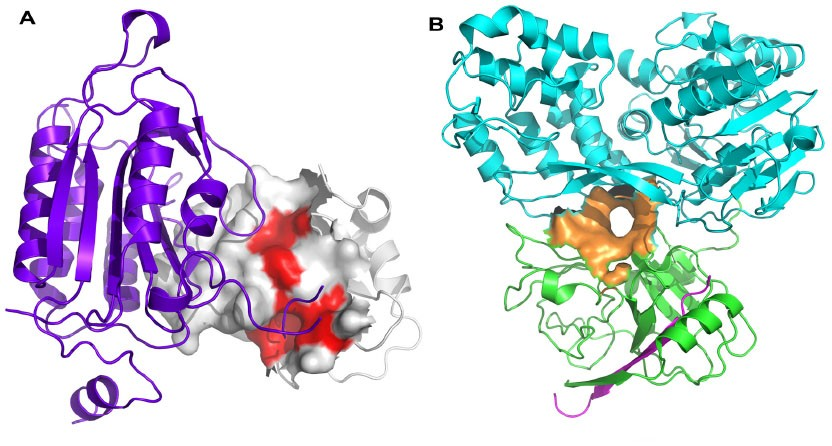
\includegraphics[width=.9\textwidth]{./images/protein-protein-int-net.jpg}
\end{minipage}\hfill
\begin{minipage}[t]{.33\textwidth}
\centering
\textbf{Infrastructure}\smallskip

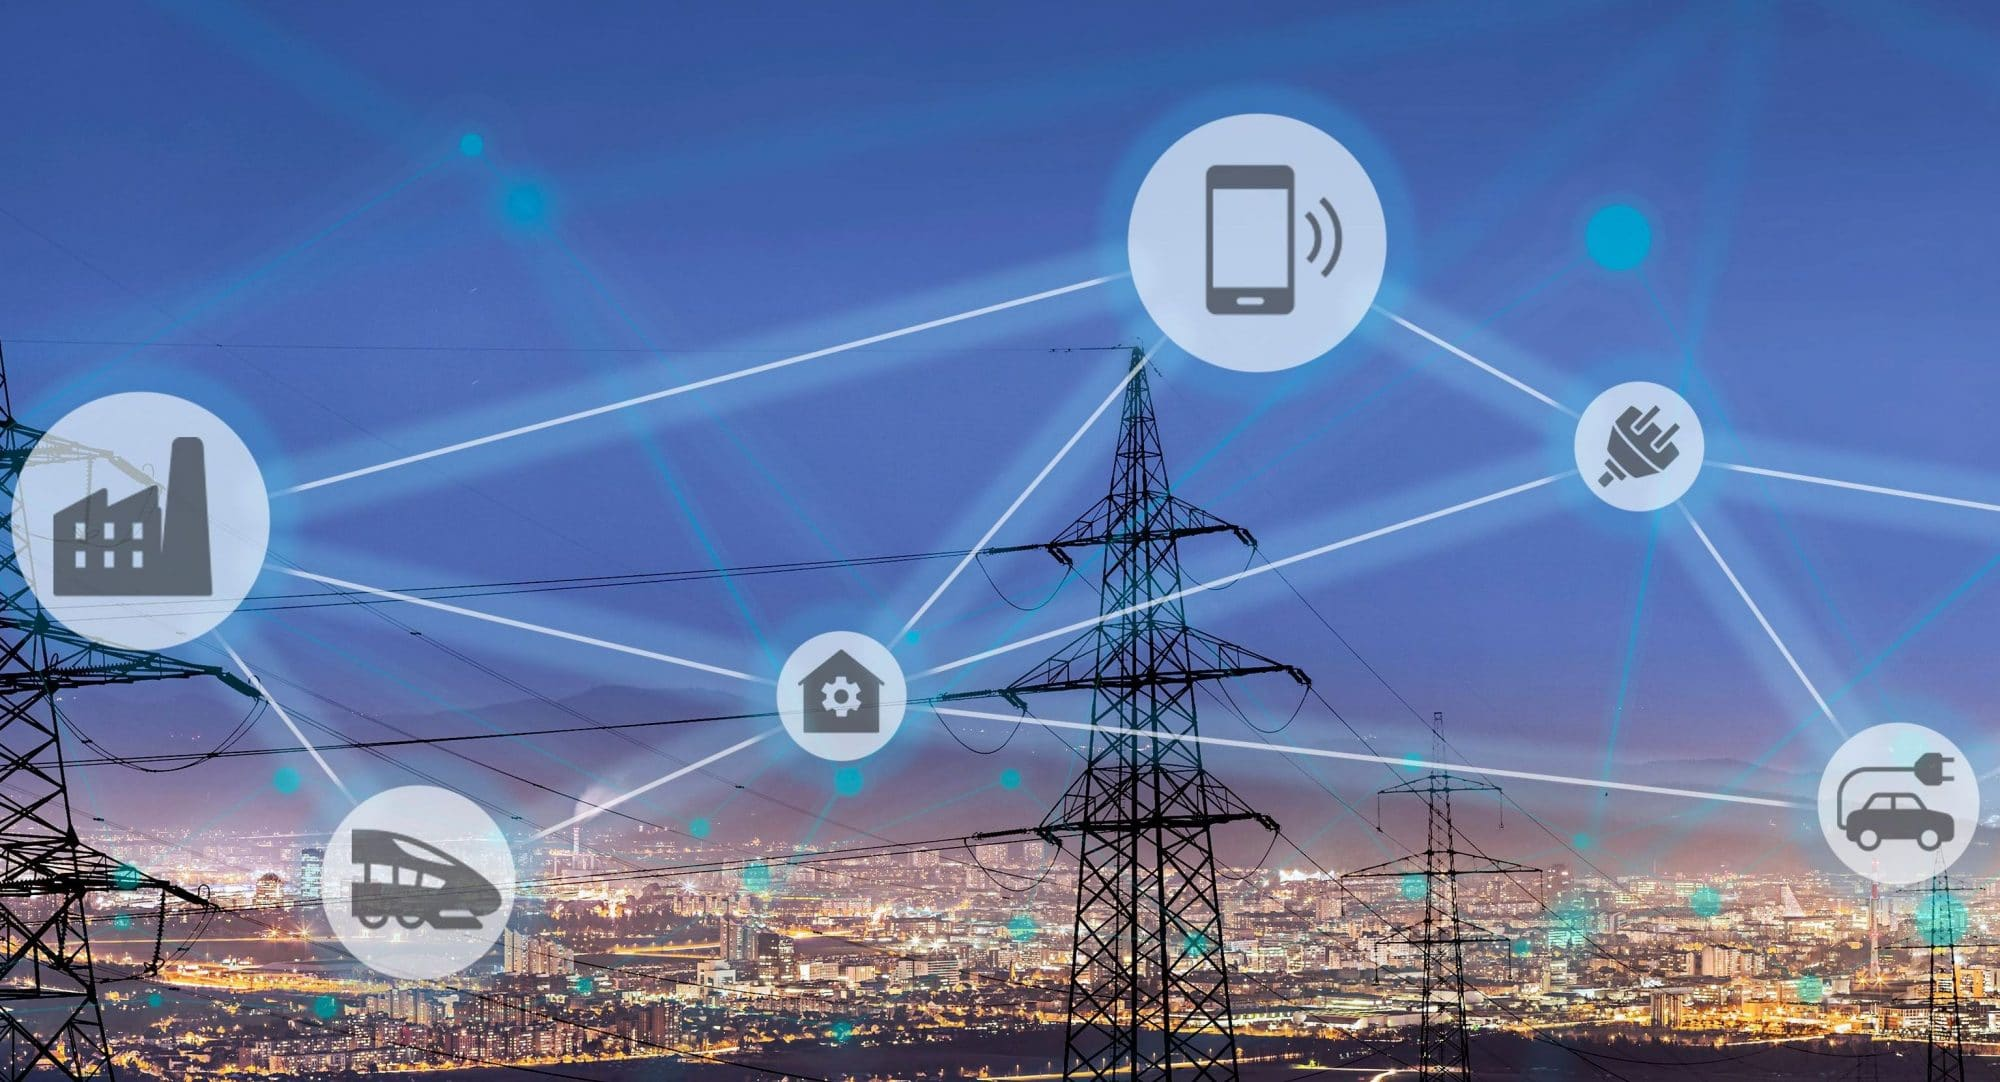
\includegraphics[width=.9\textwidth]{./images/smart-grid.jpg}
\end{minipage}\medskip

\begin{minipage}[t]{.33\textwidth}
\begin{itemize}
    \small
    \item Social networks
    \item Epidemics
\end{itemize}
\end{minipage}\hfill
\begin{minipage}[t]{.33\textwidth}
\begin{itemize}
    \small
    \item Protein-protein interactions
    \item Neural activity
\end{itemize}
\end{minipage}\hfill
\begin{minipage}[t]{.33\textwidth}
\begin{itemize}
    \small
    \item Power grids
    \item Transportation
\end{itemize}
\end{minipage}
\end{frame}

\begin{frame}[t]{Network Analysis}
\textbf{Objective:} Extract \emph{non-trivial insights} from networks.
\begin{minipage}[t]{.55\textwidth}
\begin{itemize}
    \small
\item<2-> \emph{Group structure:} community detection
\item<3-> Spread of epidemics
\item<3-> \dots
\end{itemize}\bigskip

\only<4->{In this work:}
\begin{itemize}
    \small
    \item<4-> \emph{Importance:} centrality
    \item<5-> Matching
\end{itemize}
\end{minipage}\hfill
\begin{minipage}[t]{.45\textwidth}
\only<2>{
\begin{figure}[c]
    \includesvg[svgextension=svgz,width=.7\textwidth]{./images/comm-det}
    \caption*{\tiny[Wang \etal, \textit{Hindawi}, 2019]}
\end{figure}}
\only<3>{
\begin{figure}[c]
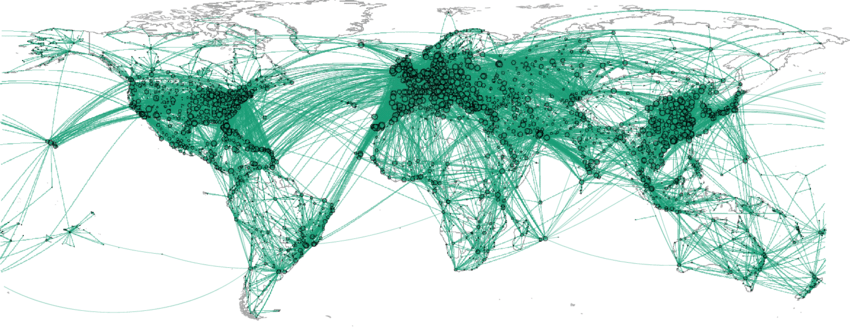
\includegraphics[width=.95\textwidth]{./images/epidemic-networks.png}
\caption*{\tiny[Matamalas \etal, \textit{Science Advances}, 2018]}
\end{figure}}
\only<4>{
\begin{figure}[c]
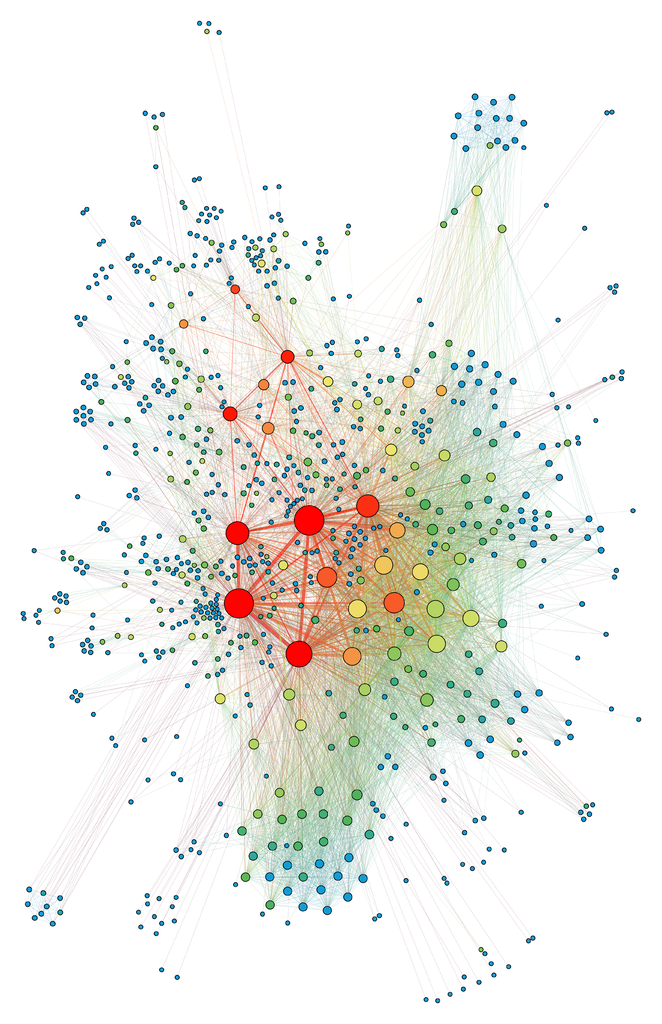
\includegraphics[width=.7\textwidth]{./images/betweenness.png}
\caption*{\tiny[\url{commons.wikimedia.org}]}
\end{figure}}
\only<5>{
\begin{figure}[c]
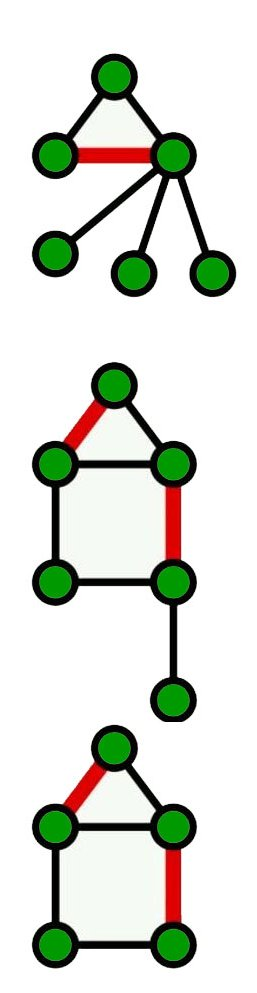
\includegraphics[width=.27\textwidth]{./images/matchings.jpg}
\caption*{\tiny[\url{www.wikiwand.com}]}
\end{figure}}
\end{minipage}
\end{frame}

\begin{frame}{Scalability Challenge}
% MASSIVE
% Today networks are Massive, show line of networ sizes
Today's networks are \emph{massive}

\begin{figure}
\begin{subfigure}[t]{.55\textwidth}
\centering
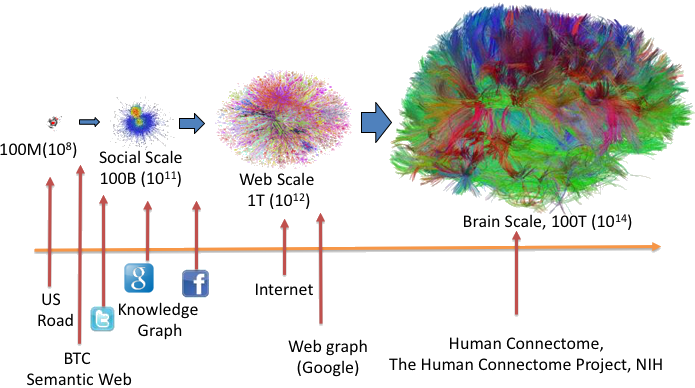
\includegraphics[width=\textwidth]{./images/networks-scale.png}
\caption*{\tiny Malewicz \etal \textit{ACM SIGMOD} 2010}
\end{subfigure}\hfill
\begin{subfigure}[t]{.45\textwidth}
\centering
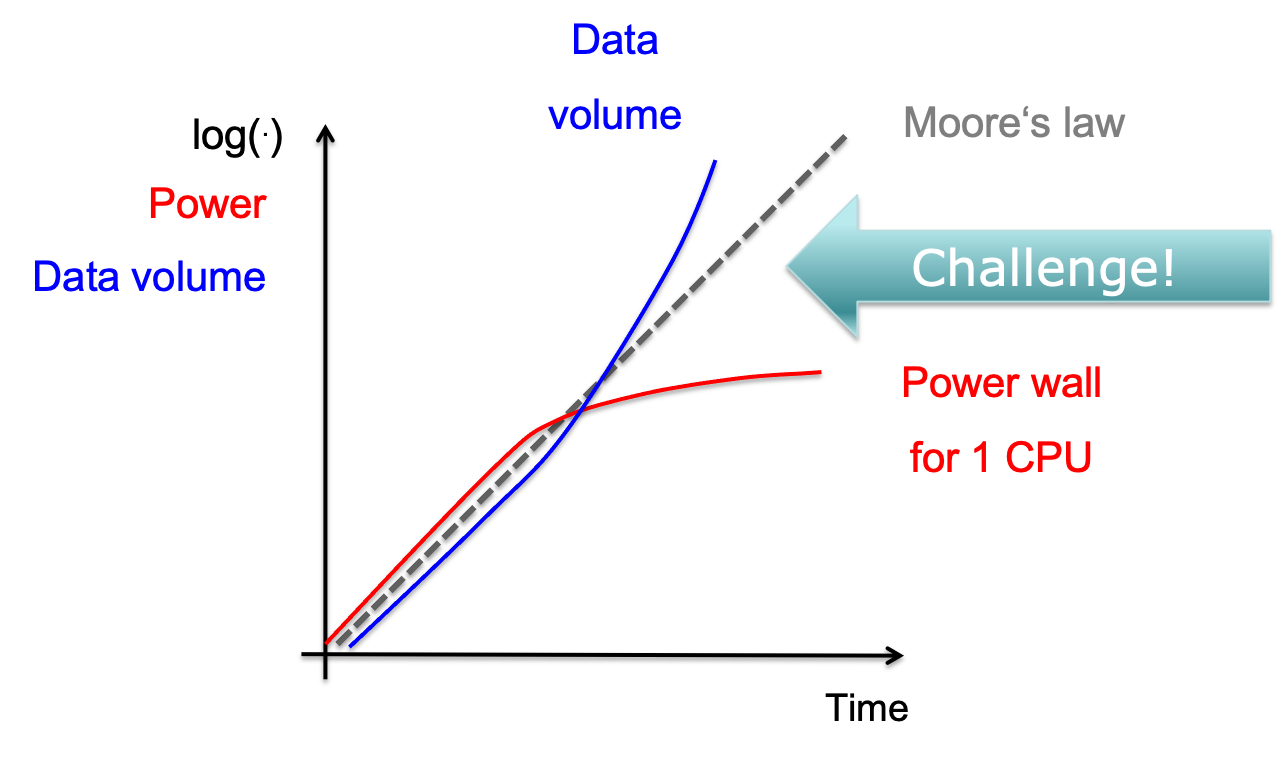
\includegraphics[width=\textwidth]{./images/scalability-challenge.png}
\end{subfigure}
\end{figure}

\begin{minipage}[t]{.5\textwidth}
\phantom{ }

\begin{itemize}
    \small
    \item Millions to billions of vertices/edges
    \item CPU speed does not keep up with data volume
    \item Need for \emph{scalable} algorithms
\end{itemize}
\end{minipage}\hfill
\begin{minipage}[t]{.5\textwidth}
\pause
Achieving \textbf{scalability}

\begin{itemize}
    \small
\item \emph{Inexact} results (approximation/heuristics)
    \item Design \emph{new metrics}
    \item \emph{Parallelism} (shared and/or distributed memory)
\end{itemize}
\end{minipage}
\end{frame}

\subsection{Contributions Overview}

\begin{frame}[t]{Overview -- Centrality}
\footnotesize
\renewcommand\theadalign{tl}
\begin{tabular}{lll}
\textbf{Problem} & \textbf{Contribution} &\\
\tikzmarkin<2>{topclos}\hspace{-1mm}Top-$k$ Closeness & \thead{Batch-dynamic algorithms, up to \emph{$10^4\times$ faster}
\\than a static recomputation.} &
\thead{\scriptsize To appear as a chapter of\\
\enquote{\scriptsize Massive Graph Analytics.}\tikzmarkend{topclos}}\\
\tikzmarkin<3>{betw}\hspace{-1mm}\thead{Betweenness\\Approximation} & \thead{General framework for parallel adaptive\\ sampling.
On 32 cores: \emph{$>60\times$ faster} than\\SotA \kadabra algorithm~\parencite{DBLP:conf/esa/BorassiN16}.}&
\thead{\parencite{DBLP:conf/europar/GrintenAM19}\\
Euro-Par 2019\\\phantom{ }\hfill\phantom{ }\tikzmarkend{betw}}\\
\tikzmarkin<4>{elclos}\hspace{-1mm}\thead{Electrical\\Closeness\\Approximation} & \thead{UST-based algorithm
to approximate\\$\diag{\Linv}$. \emph{Faster and better quality}\\than SotA.} &
\thead{\parencite{DBLP:conf/esa/AngrimanPGM20}\\ESA 2020}\\
\thead{Forest Closeness\\Approximation} & \thead{UST-based algorithm to approximate\\
$\textnormal{diag}((\Lapl + \alpha\Ident)^{-1})$. \emph{Faster and better quality}\\than SotA.} &
\thead{\parencite{DBLP:conf/sdm/GrintenAPM21}\\SDM 2021\\\phantom{ }\hfill\phantom{ }\tikzmarkend{elclos}}\\
\end{tabular}
\end{frame}

\begin{frame}[t]{Overview -- Group Centrality, Matching}
\footnotesize
\renewcommand\theadalign{tl}
\begin{tabular}{lll}
\textbf{Problem} & \textbf{Contribution} &\\
\tikzmarkin<6>[hl]{gcm2}\tikzmarkin<2>{gcm}\hspace{-2mm}\thead{Group-Closeness\\Maximization} & \thead{New heuristic
\emph{$> 100\times$ faster} than SotA.\\
Quality: comparable or better.} & \thead{\parencite{DBLP:conf/bigdataconf/AngrimanGM19}\\
IEEE BigData 2019\tikzmarkend{gcm}\tikzmarkend{gcm2}}\\
\tikzmarkin<3>{gcmapx}\hspace{-1mm}\thead{Group-Closeness\\Maximization} & \thead{\emph{First approximation algorithm.}
Higher\\ quality, trade-off with running time.} &
\thead{\parencite{DBLP:conf/alenex/AngrimanBDGGM21}\\ALENEX 2021\tikzmarkend{gcmapx}}\\
\tikzmarkin<4>{ged}\hspace{-1mm}\thead{GED-Walk} & \thead{New walk-based group centrality measure.\\
\emph{$10\times$ to $100\times$ faster}
to approximate than\\
distance-based measures.} & \thead{\parencite{DBLP:conf/alenex/AngrimanGBZGM20}\\
ALENEX 2020}\\
\thead{Group-Forest\\Maximization} & \thead{First greedy approximation algorithm.\\
\emph{Better precision for graph mining}\\\emph{applications} in disconnected graphs.} &
\thead{\parencite{DBLP:conf/sdm/GrintenAPM21}\\
SDM 2021\\\phantom{ALENEX 2020}\tikzmarkend{ged}}\\\medskip

\tikzmarkin<6>[hl]{mwm2}\hspace{-.9mm}\tikzmarkin<5>{mwm}\hspace{-2mm}Dynamic MWM & \thead{Batch-dynamic 2-approximation algorithm.\\
\emph{$10\times$ fewer traversed edges} than\\SotA~\parencite{conf/acda/AngrimanMSU21}
(ACDA 2021), $93$-$99\%$\\solution quality.} &
\thead{Under Revision\\\phantom{ }\\\hfill\\\hfill\phantom{ }\tikzmarkend{mwm}\tikzmarkend{mwm2}}\\
\end{tabular}
\end{frame}

\subsection{Centrality}

\begin{frame}[t]{(Vertex) Centrality}
\textbf{Input:} a network/graph $G = (V, E)$\smallskip

\textbf{Question:} how \emph{important} is $v\in V$?\bigskip

\only<1>{
\centering
\textbf{Main idea:} vertices with a \emph{central} position are important
\begin{figure}
\centering
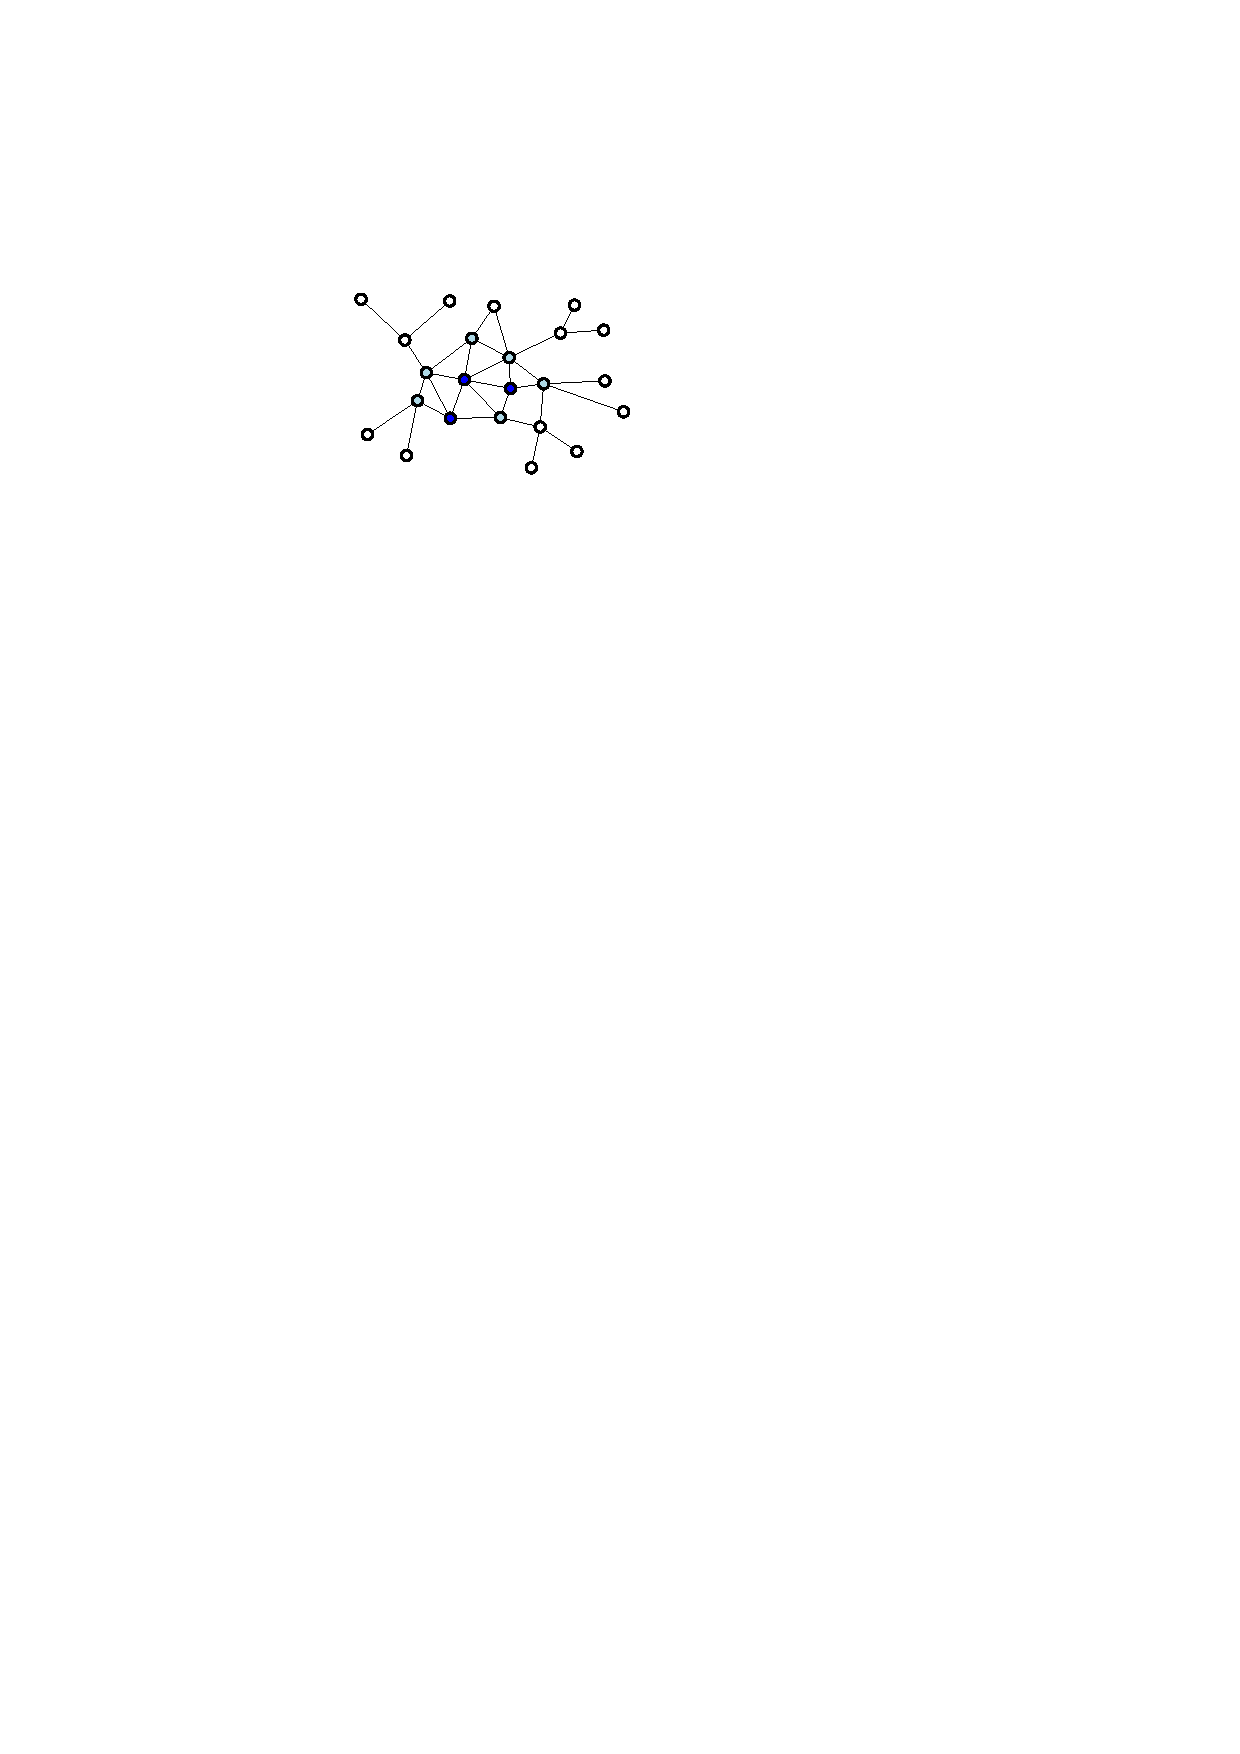
\includegraphics[width=.4\textwidth]{./images/top-k-centrality.pdf}
\end{figure}
}
\only<2>{
\begin{definition}{Centrality Measure}
Given a graph $G = (V, E)$, a centrality measure is a function:
\[
    c(\cdot) : V \to \mathbb{R},
\]
$c(u)$ is the \emph{centrality score} of $u \in V$.
\end{definition}

%Importance is \emph{relative}.\smallskip
%
%Many centrality measures were introduced.\smallskip
%
%Choice of $c(\cdot)$ depends on the \emph{application}.
}
\end{frame}

%\begin{frame}[t]{Centrality}
%\framesubtitle{Different Applications -- Different Measures}
%\vspace{-5mm}
%\begin{figure}[t]
%\includegraphics[width=.8\textwidth]{./images/jakarta.pdf}
%\caption*{\tiny Klipper \etal, AGILE GIScience Ser., 2, 4, 2021}
%\end{figure}
%\end{frame}

\subsection{Group Centrality}

\begin{frame}[t]{Group Centrality}
\footnotesize
\textbf{Input:} graph $G = (V, E)$, integer $1 \le k < n$.\medskip

\textbf{Question:} most central \emph{group of vertices} $S \subset V$ s.t. $|S| = k$.
\bigskip

\only<1>{
Not the \emph{top-$k$} most individually central vertices\dots

\begin{minipage}[t]{.5\textwidth}
\begin{figure}[t]
\centering
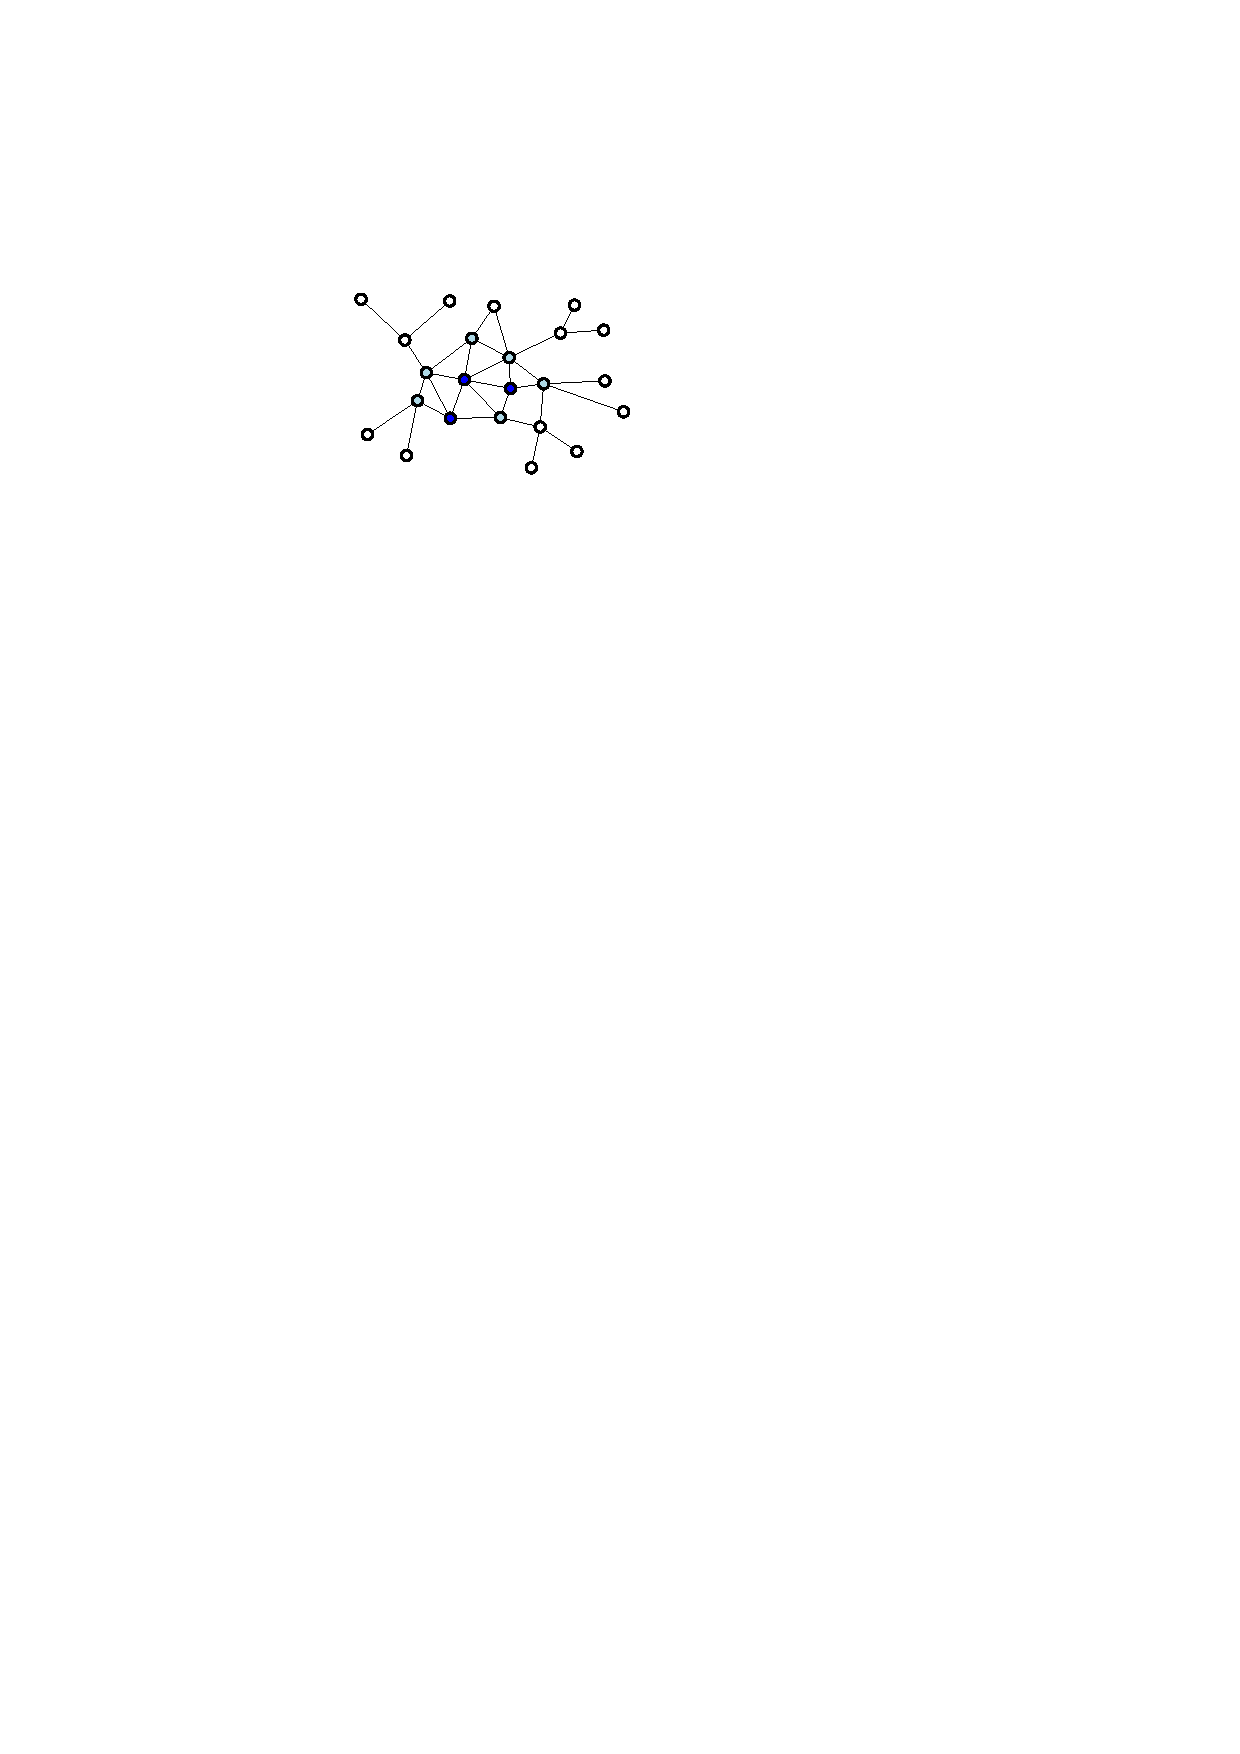
\includegraphics[width=.8\textwidth]{./images/top-k-centrality.pdf}
\end{figure}
\end{minipage}\hfill
\begin{minipage}[t]{.5\textwidth}
\onslide<1>{\begin{figure}[t]
\centering
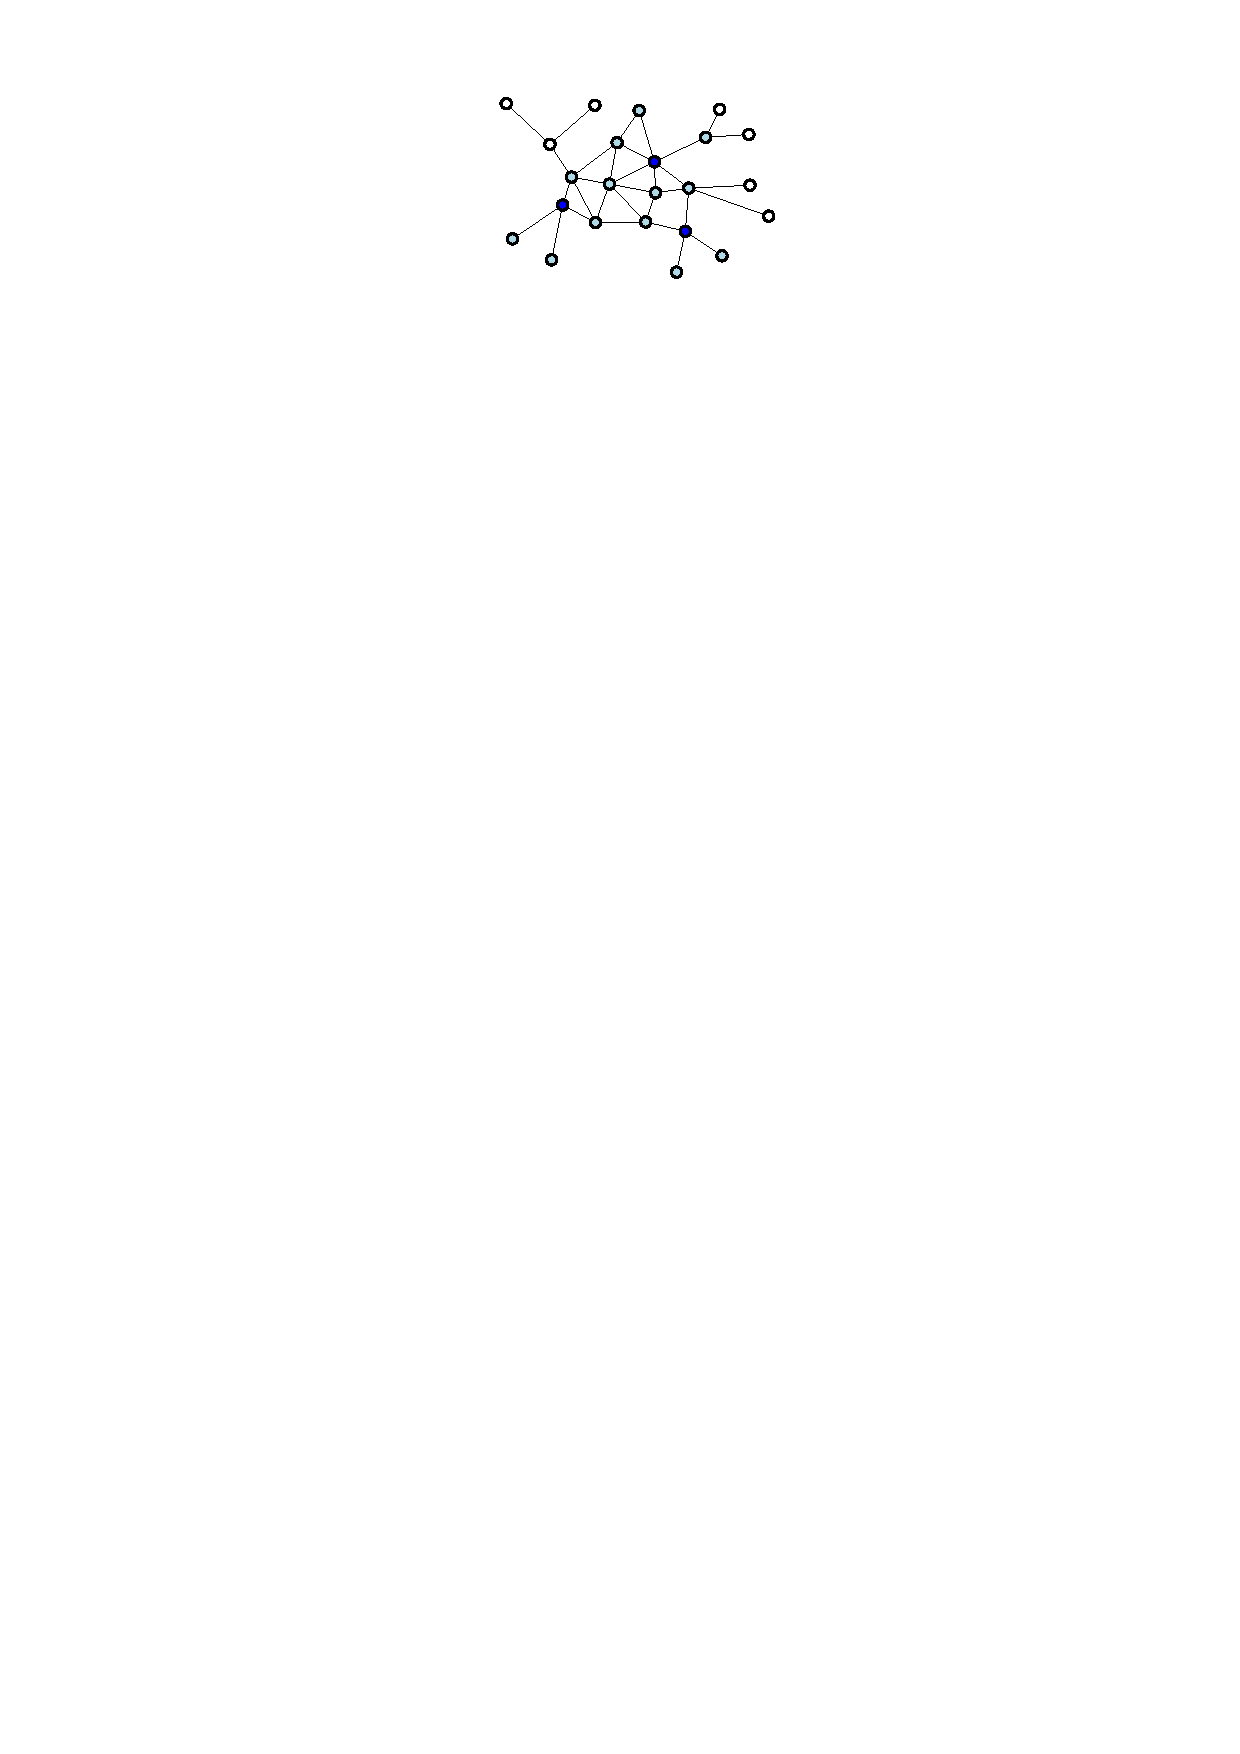
\includegraphics[width=.8\textwidth]{./images/group-centrality.pdf}
\end{figure}}
\end{minipage}\medskip

\onslide<1>{\hfill\dots but the most central \emph{group} as a whole!}
}

\only<2->{
\vspace{-2mm}
\begin{definition}{Group Centrality Measure}
Given a graph $G = (V, E)$, a group centrality measure $g(\cdot)$ is
a set function
\[
    g : \mathcal{P}(V) \to \mathbb{R},
\]
$g(S)$ is the \emph{group centrality score} of $S \subset V$.
\end{definition}
}
\onslide<3->{
\begin{minipage}[t]{.5\textwidth}
\vspace{-2mm}
\begin{block}{\footnotesize Group Centrality Maximization Problem}
\footnotesize
\textbf{Input:} Graph $G = (V, E)$, integer $1 \le k < n$,
group centrality measure $g(\cdot)$.\medskip

\textbf{Output:}
\[
    S^\star := \argmax_{S \subset V, |S| = k} g(S).
\]
\end{block}
\end{minipage}\hfill
\begin{minipage}[t]{.45\textwidth}
\smallskip

Popular group centrality measures:\medskip

\begin{itemize}
\footnotesize
    \item Maximization problem is \np-hard
    \item Typical maximization strategy: greedy ascent or heuristics
\end{itemize}
\end{minipage}
}
\end{frame}


\subsection{Group-Closeness}

\begin{frame}[t]{Group-Closeness}
Given a graph $G = (V, E)$
\begin{definition}{Group-closeness of $S \subset V$}
\begin{minipage}[t]{.5\textwidth}
Group-farness:
\[
\gfarn(S) := \sum_{u \in V \setminus S}d(S, u),
\quad\to
\]
where $d(S, u) = \min_{s \in S}d(s, u)$.
\end{minipage}\hfill
\begin{minipage}[t]{.5\textwidth}
Group-closeness:
\[
\gclos(S) := \frac{n}{\gfarn(S)}.
\]
\end{minipage}

\end{definition}

\only<1>{\begin{figure}
\centering
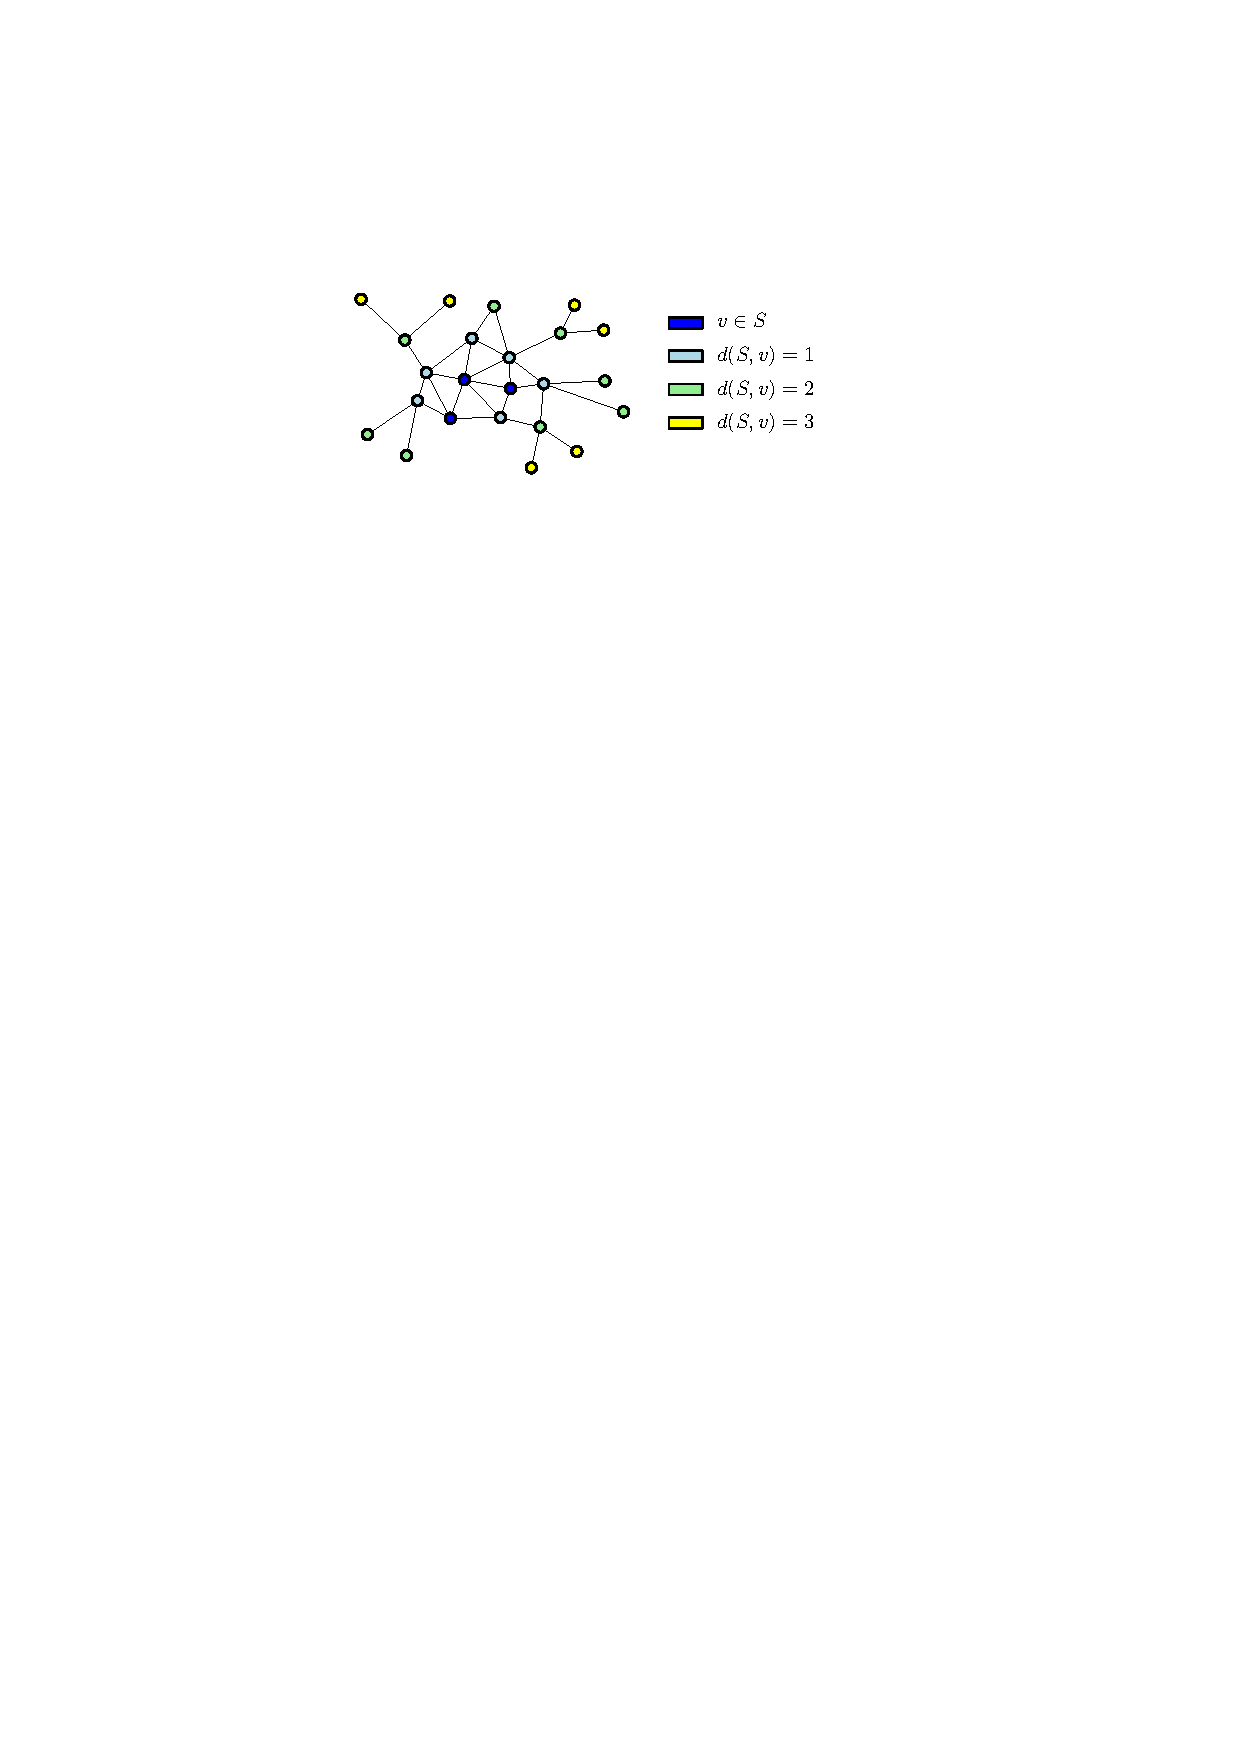
\includegraphics[width=.6\textwidth]{./images/group-farness.pdf}
\end{figure}
}
\only<2->{
Finding $S^\star$ with maximum $\gclos(S)$ is \np-hard~\parencite{DBLP:conf/adc/ChenWW16}.
\medskip

\emph{SotA:} greedy ascent heuristic~\parencite{DBLP:conf/alenex/BergaminiGM18}.\bigskip

\onslide<3->{
\small
\begin{minipage}[t]{.5\textwidth}
    \faThumbsOUp\ Nearly-optimal solutions (often)\smallskip

    \faThumbsOUp\ Good scalability \wrt $k$
\end{minipage}\hfill
\begin{minipage}[t]{.5\textwidth}
    \faThumbsODown\ High overhead\smallskip

    \faThumbsODown\ Cannot correct \enquote{bad} choices
\end{minipage}}
}
\end{frame}

\section{Local Search for Group-Closeness}
\subsection{Introduction}

\begin{frame}[t]{Local Search for Group-Closeness}
\small
\textbf{Assumption} (for now): we have a group $S$, $|S| = k$.\smallskip

\textbf{Idea:} increase $\gclos(S)$ by \emph{vertex exchanges} between
$S$ and $\overline{S}$.\bigskip

%\begin{block}{\small Notation: Vertex Exchange}
%\hfill$\Suv := (S\cup\set{v})\setminus\set{u}$\hfill$\Su := S \setminus\set{u}$\hfill
%$\Sv := S \cup \set{v}$\hspace{1.5cm}
%\end{block}\bigskip

\begin{minipage}[t]{.4\textwidth}
\onslide<2->{
\begin{block}{\textbf{New simple algorithm:}}

Initialize $S$ randomly, then

\begin{enumerate}
    \small
    \item Find the best exchange:
    \[
        \argmin_{u\in S,\ v\in\overline{S}}\ \gfarn\roundb{(S \cup \set{v}) \setminus \set{u}}
    \]
    \item Update $S \gets (S \cup \set{v}) \setminus \set{u}$
    \item Repeat until $\gfarn(S)$ did not decrease
\end{enumerate}
\end{block}}
\end{minipage}\hfill
\begin{minipage}[t]{.55\textwidth}
\onslide<3->{\textbf{Issue:}
\begin{itemize}
    \small
\item Computing $\gfarn(S)$ naively requires a SSSP
\item Impractical to do for all exchanges
\end{itemize}\medskip

\textbf{Solution:} new algorithm \parencite{DBLP:conf/bigdataconf/AngrimanGM19}
\begin{itemize}
    \small
\item[\faHandORight] \emph{Separate} vertex insertions and removals
        (no need to consider exchanges)
\end{itemize}
}
\end{minipage}
\end{frame}

\subsection{Insertions}

\begin{frame}[t]{Insertions -- Bound Farness Decrease}
\small
\textbf{Need:} decrease in farness
\emph{$\deltafarnm(v) := \gfarn(S) - \gfarn(\Sv)$} $\forall v\in \overline{S}$.
\smallskip

\textbf{Idea:} use a shortest-path DAG from $S$.

\begingroup\centering
\only<1>{\begin{tikzpicture}[scale=.7]}
\only<2->{\begin{tikzpicture}[draw=lightgray,scale=.7]}
\renewcommand{\darkorange}{\emphcolor}

\drawgraphcontour
\drawgroupcontour

\simplenode{\nodeida}{\coorda}
\simplenode{\nodeidb}{\coordb}
\simplenode{\nodeidc}{\coordc}
\simplenode{\nodeidd}{\coordd}
\simplenode{\nodeide}{\coorde}
\simplenode{\nodeidf}{\coordf}

\simplenode{\nodeidg}{\coordg}
\only<1>{\simplenode{\nodeidh}{\coordh}}
\only<2->{\colortextnode{\nodeidh}{\nodeidh}{$v$}}
\simplenode{\nodeidi}{\coordi}
\simplenode{\nodeidj}{\coordj}

\simplenode{\nodeidk}{\coordk}
\only<1>{
\simplenode{\nodeidl}{\coordl}
\simplenode{\nodeidm}{\coordm}
\simplenode{\nodeidn}{\coordn}
}
\only<2->{
\colornode{\nodeidl}{\coordl}
\colornode{\nodeidm}{\coordm}
\colornode{\nodeidn}{\coordn}
}
\simplenode{\nodeido}{\coordo}

\only<1>{
\simplenode{\nodeidp}{\coordp}
\simplenode{\nodeidq}{\coordq}
\simplenode{\nodeidr}{\coordr}
}
\only<2->{
\colornode{\nodeidp}{\coordp}
\colornode{\nodeidq}{\coordq}
\colornode{\nodeidr}{\coordr}
}

\edgecoords

\draw[->] (sg1) -- (ng3);
\draw[->] (sg11) -- (ng21);
\draw[->] (sg2) -- (ng4);
\draw[->] (sg3) -- (ng2);
\draw[->] (sg4) -- (ng1);
\draw[<-] (sg5) -- (sg3b);
\draw[<-] (sg6) -- (sg2b);

\draw[->] (ng1b) -- (ng5);
\only<1>{
\draw[->] (ng2b2) -- (ng6);
\draw[->] (ng2b) -- (ng7);
\draw[->] (ng2b1) -- (ng81);
}
\only<2->{
\draw[->,blue,thick] (ng2b2) -- (ng6);
\draw[->,blue,thick] (ng2b) -- (ng7);
\draw[->,blue,thick] (ng2b1) -- (ng81);
}
\draw[->] (ng3b) -- (ng8);
\draw[->] (ng3b1) -- (ng9);

\only<1>{
\draw[->] (ng6b) -- (ng10);
\draw[->] (ng7b) -- (ng11);
\draw[->] (ng7b1) -- (ng12);
}
\only<2->{
\draw[->,blue,thick] (ng6b) -- (ng10);
\draw[->,blue,thick] (ng7b) -- (ng11);
\draw[->,blue,thick] (ng7b1) -- (ng12);
};

\only<2->{
    \node[] at (10, -1.5) {\textnormal{Here:} \emph{$|\deltafarnm(v)| = 7$}};
}
\end{tikzpicture}
\endgroup\par


\pause
\emph{$D_v$}: vertices reachable from $v$ in the DAG. It holds:
$\deltafarnm(v) \ge |\emph{D_v}|\cdot d(S, v).$
%\begin{itemize}
%    \small
%    \item Note: if $G$ unweighted and $v \in N(S)$, then it holds: $\deltafarnm(v) = |\emph{D_v}|$.
%\end{itemize}

\pause
\begin{block}{\vspace*{-3ex}}
\textcolor{red}{\warning} Computing $D_v\ \forall v\in\overline{S}\ \Rightarrow$ transitive closure of a DAG,
$\tilde{\Oh}(n^{2.373})$ time.\medskip

\faHandORight\ Randomized algorithm~\parencite{DBLP:journals/jcss/Cohen97}:
approx. $D_v\ \forall v\in \overline{S}$ in $\Oh(n + m)$ time.
\end{block}
\end{frame}


\subsection{Removals -- Data Structures}

\begin{frame}{Removals -- Data Structures}
\small
For each $x \in \overline{S}$ we store:
\begin{itemize}
    \small
\item $d_S(x) = d(S, x)$ \textbf{and} the nearest vertex $r_x \in S$\smallskip

\quad$\to\textcolor{HUBblue}{R_v := \set{x \in \overline{S} : d(v, x) = d_S(x)}}\ \forall v\in S$

\item $d_S'(x) = d(S \setminus \set{r_x}, x)$ \textbf{and} the nearest vertex $r_x' \in S \setminus \set{r_x}$\smallskip

\quad$\to\textcolor{HUBorange}{R_v' := \set{x \in \overline{S} : d(v, x) = d_S'(x)}}\ \forall v\in S\setminus\set{r_x}$
\end{itemize}

\begin{figure}
\centering
\begingroup\centering
\begin{tikzpicture}
\small

\coordinate (r1) at (2,2.4);
\coordinate (r2) at (6.25,2.85);
\coordinate (r3) at (8,2.8);

\node[] at (2, 3.8) {$v, w\in S$};
\draw (r1) circle [radius=3pt] coordinate (w);
\draw (w) node [above=.15cm] {$v$};
\draw (r2) circle [radius=3pt];
\draw (r2) node [above=.15cm] {$w$};

\node[HUBblue, draw, shape=rectangle, minimum width=2.55cm, minimum height=1.5cm, anchor=center,rounded corners=20pt,thick] at (r1) {};
\node[HUBblue] at ([yshift=-15pt]w) {$x: r_x = v$};
\node [HUBblue, draw, shape=rectangle, minimum width=2.5cm, minimum height=2.0cm, anchor=center,rounded corners=25pt,thick] at  (r2) {};
\node[HUBblue] at ([yshift=-15pt]r2) {$x: r_x = w$};

\draw[HUBorange, rounded corners=30pt,dashed,thick]
  (0,1.1) rectangle ++(4,2.2);
\node[HUBorange] at ([yshift=-30pt]w) {$x : r_x' = v$};
\draw[HUBorange, rounded corners=40pt,dashed,thick]
  (4,1.3) rectangle ++(3.5,3);
\node[HUBorange] at ([xshift=-20pt,yshift=-35pt]r2) {$x : r_x' = w$};

\end{tikzpicture}
\endgroup

\end{figure}
\end{frame}

\subsection{Removals}

\begin{frame}[t]{Vertex Removal}
\small
\textbf{Exact} farness increase $\forall u\in S$: \emph{$\deltafarnp(u) := \sum_{x\in R_u}d_S'(x) - d_S(x)$}.\smallskip

Pick vertex $u\in S$ that minimizes $\deltafarnp(u)$.

\begin{center}
    \onslide<2->{\begingroup\centering
\begin{tikzpicture}
\small
\coordinate (r1) at (2,2.4);
\coordinate (r2) at (6.25,2.85);
\coordinate (r3) at (8,2.8);
\coordinate (l1) at (.1, 4);
\coordinate (l2) at (.55, 4);
\coordinate (l3) at (.1, 3.6);
\coordinate (l4) at (.55, 3.6);
\coordinate (u1) at ([xshift=.75cm, yshift=-.45cm]r2);
\coordinate (w1) at ([xshift=.75cm, yshift=.3cm]r1);
\coordinate (w2) at ([xshift=.85cm, yshift=-.3cm]w1);
\coordinate (w3) at ([xshift=.95cm, yshift=.4cm]w2);
\path (w) ++(30:3pt) coordinate (pw1);
\path (w1) ++(180:3pt) coordinate (pw2);
\path (w1) ++(0:3pt) coordinate (pw3);
\path (w2) ++(160:3pt) coordinate (pw4);
\path (w2) ++(0:3pt) coordinate (pw5);
\path (w3) ++(185:4pt) coordinate (pw6);
\path (r2) ++(325:3pt) coordinate (pu1);
\path (u1) ++(145:3pt) coordinate (pu2);
\path (u1) ++(30:4pt) coordinate (pu3);
\path (r3) ++(190:3pt) coordinate (pu6);

\node[cyan, draw, shape=rectangle, minimum width=2.55cm, minimum height=1.5cm, anchor=center,rounded corners=20pt,thick] at (r1) {};
\onslide<-5>{
\node [HUBred, draw, shape=rectangle, minimum width=2.5cm, minimum height=2.0cm, anchor=center,rounded corners=25pt,thick] at  (r2) {};
\node [cyan,draw, shape=rectangle, minimum width=1cm, minimum height=1.3cm, anchor=center,rounded corners=10pt,
thick] at (r3) {};
\draw[HUBorange, rounded corners=40pt,dashed,thick]
  (4,1.3) rectangle ++(3.5,3);
\node[draw,cyan,shape=rectangle, rounded corners=30pt,dashed,thick, minimum width=3.8cm, minimum height=2.5cm]
at ([xshift=.1cm,yshift=-.3cm]r1) {};
\node [cyan,draw, shape=rectangle, minimum width=2cm, minimum height=1.5cm, anchor=center,rounded corners=15pt,
thick, dashed] at ([xshift=.5cm]r3) {};
}
\onslide<6->{
\node [cyan,draw, shape=rectangle, minimum width=4.9cm, minimum height=1.5cm, anchor=center,rounded corners=15pt,
thick, dashed] at ([xshift=-.95cm]r3) {};
\node [cyan,draw, shape=rectangle, minimum width=3cm, minimum height=1.3cm, anchor=center,rounded corners=10pt,
thick] at ([xshift=-1cm]r3) {};

\node[draw,cyan,shape=rectangle, rounded corners=30pt,dashed,thick, minimum width=4.4cm, minimum height=2.5cm]
at ([xshift=.4cm,yshift=-.3cm]r1) {};
}

\only<3-4>{
    \draw (w3) circle [radius=3pt];
    \draw (u1) circle [radius=3pt];
}
\only<5>{
    \customcolornode{w31}{w3}{cyan};
    \customcolornode{u11}{u1}{cyan};
}

\draw (r1) circle [radius=3pt] coordinate (w);
\draw (w) node [below=.1cm] {$a$};
\onslide<3-5>{
\draw (w1) circle [radius=3pt];
\draw (w2) circle [radius=3pt];
\draw (w2) node [below=.1cm] {$x$};
\draw (w3) node [below=.15cm] {$y$};

\draw[-] (pw1) -- (pw2);
\draw[-] (pw3) -- (pw4);
\draw[densely dotted, ultra thick] (pw5) -- (pw6);
}

\draw (r3) circle [radius=3pt];
\draw (r3) node [below=.15cm] {$c$};

\only<-5>{
\draw (r2) circle [radius=3pt];
\draw (r2) node [above=.1cm] {$u$};
\draw (r2) node [below left=.65cm] {\textcolor{HUBred}{$R_u$}};
\draw (r2) node [below left=1.3cm] {\textcolor{HUBorange}{$R_{u}'$}};
}
\onslide<3-5>{
\draw (u1) node [below=.15cm] {$z$};

\draw[-] (pu1) -- (pu2);
\draw[dashed, ultra thick] (pu3) -- (pu6);

%\draw[densely dotted, ultra thick] (l1) -- (l2);
%\draw[dashed, ultra thick] (l3) -- (l4);
%\node [right=.1cm of l2,align=left] {$d_S'$-boundary pair};
%\node [right=.1cm of l4,align=left] {$d_S$-boundary pair};
}

\only<4-5>{
\draw (u1) node [above=.2cm] {$d_S(c)$};
\draw (w3) node [above=.15cm] {$d_S'(x)$};
}
\end{tikzpicture}
\endgroup\par
}
\end{center}\medskip

\begin{itemize}
    \small
    \item<2-> Vertices $\textcolor{HUBred}{z \in R_u: d_S(z) \gets d_S'(z)}$
    \smallskip

    \faHandORight\ need to re-compute $d_S'(v)$ for all
    $v \in \textcolor{HUBred}{R_u} \cup \textcolor{HUBorange}{R_u'}$\medskip

%    \item<3-> Boundary pairs: $\pair{x}{y} : d_S'(y) \gets b(x, y)$
    \item<3-> Update $d_S'(\cdot)$
        with Dijkstra-like algo from \textcolor{cyan}{boundary vertices}
\end{itemize}
\end{frame}

\subsection{\growshrink Algorithm}

\begin{frame}[t]{\growshrink Algorithm}
Issue: cannot \enquote{escape} from local optima.

%\item[\faThumbsODown] Underestimates $\deltafarnm(v)$ for vertices with high DAG depth
%\vspace{-5mm}
%\begin{center}
%    \begingroup\centering
\begin{tikzpicture}[scale=.8]
\drawgraphcontour
\drawgroupcontour

\simplenode{\nodeida}{\coorda}
\simplenode{\nodeidb}{\coordb}
\simplenode{\nodeidc}{\coordc}
\simplenode{\nodeidd}{\coordd}
\simplenode{\nodeide}{\coorde}
\simplenode{\nodeidf}{\coordf}

\simplenode{\nodeidg}{\coordg}
\customcolornode{\nodeidh}{\coordh}{red}
\simplenode{\nodeidi}{\coordi}
\simplenode{\nodeidj}{\coordj}

\simplenode{\nodeidk}{\coordk}
\customcolornode{\nodeidl}{\coordl}{red}
\node[] at ([yshift=.4cm]\coordn) {$v$};
\customcolornode{\nodeidm}{\coordm}{red}
\customcolornode{\nodeidn}{\coordn}{cyan}
\simplenode{\nodeido}{\coordo}

\customcolornode{\nodeidp}{\coordp}{red}
\customcolornode{\nodeidq}{\coordq}{cyan}
\customcolornode{\nodeidr}{\coordr}{cyan}

\node[align=left] at (12, .25) {\textnormal{Forward contrib.}};
\node[align=left] at (12, -.25) {\textnormal{Backward contrib.}};
\node[align=left] at (10, -2) {\normalsize$\deltafarnm(v) \ge |\textcolor{cyan}{D_v}|\cdot d(S, v)$};

\coordinate[] (f1) at (9.5, .25);
\coordinate[] (f2) at (10.25, .25);
\coordinate[] (b1) at (9.5, -.25);
\coordinate[] (b2) at (10.25, -.25);
\draw[thick,cyan] (f1) -- (f2);
\draw[thick,red] (b1) -- (b2);

\edgecoords

\draw[->] (sg1) -- (ng3);
\draw[->] (sg11) -- (ng21);
\draw[->] (sg2) -- (ng4);
\draw[->] (sg3) -- (ng2);
\draw[->] (sg4) -- (ng1);
\draw[<-] (sg5) -- (sg3b);
\draw[<-] (sg6) -- (sg2b);

\draw[->] (ng1b) -- (ng5);
\draw[->,red,thick] (ng2b2) -- (ng6);
\draw[->,red,thick] (ng2b) -- (ng7);
\draw[->,red,thick] (ng2b1) -- (ng81);
\draw[->] (ng3b) -- (ng8);
\draw[->] (ng3b1) -- (ng9);

\draw[->,red,thick] (ng6b) -- (ng10);
\draw[->,cyan,thick] (ng7b) -- (ng11);
\draw[->,cyan,thick] (ng7b1) -- (ng12);

\end{tikzpicture}
\endgroup\par

%\end{center}

\bigskip
\textbf{Solution:} \growshrink algorithm
\begin{itemize}
    \small
    \item allow $S$ to \emph{grow} (temporarily) to size $\emph{k + h}$\dots
    \item\dots and then \emph{shrink} it back to size $k$.\smallskip
\end{itemize}

Strategy for choosing $h$:
\begin{itemize}
    \small
\item[\faHandORight] Constant $h \ge 1$
\item[\faHandORight] $h = \diam(G)/k^p$, for a fixed $p > 0$
\end{itemize}
\end{frame}


\subsection{Experiments}

\begin{frame}
\centering
\vfill\Huge\textbf{\textcolor{HUBblue}{Experiments}}\vfill
\end{frame}

\begin{frame}[t]{\growshrink\ -- Unweighted Graphs}
\small
\begin{figure}
\centering
\begin{subfigure}[t]{\textwidth}
\centering

\includegraphics{../sources/plots/local-search-heu/legend-h-p-params.pdf}
\end{subfigure}\smallskip

\begin{subfigure}[t]{.5\textwidth}
\centering
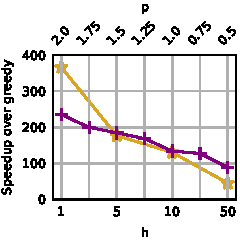
\includegraphics{../sources/plots/local-search-heu/speedups-h-p-params.pdf}
\end{subfigure}\hfill
\begin{subfigure}[t]{.5\textwidth}
\centering
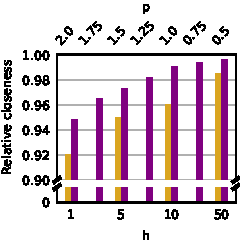
\includegraphics{../sources/plots/local-search-heu/quality-h-p-params.pdf}
\end{subfigure}
\caption*{\footnotesize $k = 10$, geometric mean over 11 real-world networks, up to 27M edges.}
\end{figure}

\onslide<2->{
\begin{tikzpicture}[remember picture,overlay]
    \node[circle,minimum size=.5cm] at (current page.center) [
    draw,align=center,anchor=center,xshift=-1.55cm,yshift=-.06cm,red, very thick]
{};
    \node[circle,minimum size=.5cm] at (current page.center) [
    draw,align=center,anchor=center,xshift=4.3cm,yshift=1.6cm,red, very thick]
{};
\end{tikzpicture}

With $p = 0.75$:\smallskip

\quad\faThumbsOUp\ \emph{$\onedigit{\gsPSevenFiveKSpeed}\times$ faster} than greedy,
\emph{$\onedigit{\gsPSevenFiveKQualNum}\%$ quality}
}
\end{frame}

\begin{frame}[t]{\growshrink\ -- Weighted Graphs}
\begin{figure}
\centering
\begin{subfigure}[t]{\textwidth}
\centering

\includegraphics{./images/legend_weighted.pdf}
\end{subfigure}\smallskip

\begin{subfigure}[t]{.5\textwidth}
\centering
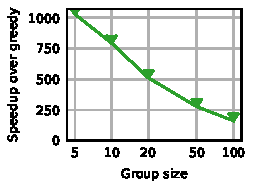
\includegraphics{./images/speedups_weighted.pdf}
\end{subfigure}\hfill
\begin{subfigure}[t]{.5\textwidth}
\centering
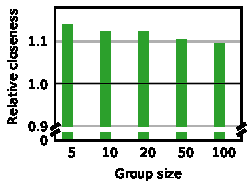
\includegraphics{./images/quality_weighted.pdf}
\end{subfigure}
\caption*{\footnotesize Geometric mean over 14 US road networks, up to 380K edges.}
\end{figure}

For $k \le 100$ and \wrt greedy:\smallskip

\begin{itemize}
    \small
    \item[\faThumbsOUp] Always $> 100\times$ faster
    \item[\faThumbsOUp] Solutions with \emph{higher quality}
\end{itemize}
\end{frame}

\subsection{Conclusions}

\begin{frame}{Conclusions}
\framesubtitle{Local Search for Group-Closeness}
\textbf{Problem: Group-Closeness Maximization}
\begin{itemize}
    \small
    \item \np-hard optimization problem
    \item Existing algorithms are not scalable
    \item SotA: greedy ascent~\parencite{DBLP:conf/alenex/BergaminiGM18}
\end{itemize}\medskip

\textbf{\growshrink}
\begin{itemize}
    \small
\item Weighted graphs: \emph{better quality} and $\emph{>100\times}$ faster
\item Unweighted graphs $k = 10$: \emph{$> 99\%$} quality and $\emph{>100\times}$ faster
\item Networks with \emph{$>300$M edges} in \emph{$\approx 10$ min} ($k = 10$).
\end{itemize}\medskip

%\textbf{Local-Swaps}
%\begin{itemize}
%\small
%\item Single swaps restricted to the \emph{neighborhood} of $S$
%\item For small groups ($k \le 10$): $\approx 80\%$ quality, $>1000\times$ faster
%\end{itemize}\pause\medskip

%\textbf{Group-Closeness Approximation?}
\end{frame}


%\subsection{Group-Closeness Approximation}
%
%\begin{frame}[t]{Group-Closeness Approximation}
%\footnotesize
%Group-closeness maximization $\longleftrightarrow$ \emph{metric $k$-Median} problem:\medskip
%
%\textbf{Approximation algorithm} for metric $k$-Median~\parencite{DBLP:journals/siamcomp/AryaGKMMP04}:
%\begin{itemize}
%\footnotesize
%\item Based on local search
%\item $(1 + \frac{1}{e})$-approximation~\parencite{DBLP:journals/tmc/DAngeloDNP16}
%\end{itemize}\medskip
%
%\textbf{Approximation algorithm} for group-closeness~\parencite{DBLP:conf/alenex/AngrimanBDGGM21}:
%\begin{itemize}
%\footnotesize
%\item $\frac{e}{(e + 1)}$-approximation (undirected)
%\item $4\cdot n^{-\epsilon}$ (directed)
%\end{itemize}
%
%\begin{minipage}[t]{.5\textwidth}
%\begin{itemize}
%\footnotesize
%\item[\faThumbsOUp] Always yields the best quality
%\item[\faThumbsODown] $10\times$ to $100\times$ slower than heuristics
%\end{itemize}\bigskip
%\end{minipage}\hfill
%\begin{minipage}[t]{.5\textwidth}
%\begin{itemize}
%    \footnotesize
%    \item[\faHandORight] Time vs quality trade-off
%    \item[\faHandORight] Approximation viable only in networks with moderate size
%\end{itemize}
%\end{minipage}
%\end{frame}

\section{Dynamic Matching}

\begin{frame}
\centering
\vfill\Huge\textbf{\textcolor{HUBblue}{Dynamic Matching}}\vfill
\end{frame}

\subsection{Introduction}

\begin{frame}{Matching}
\small\medskip

\begin{definition}{\small Matching}
A matching $M \subseteq E$: set of edges not sharing any endpoints.
\end{definition}

$M$ is a \emph{Maximum Weighted Matching} (MWM) iff $M$ has the highest
possible weight.\medskip

\textbf{Weight} of $M$: $\sum_{e\in M}w(e)$.\medskip

\begin{figure}
\centering
\begin{tikzpicture}[scale=.8]
\coordinate (a) at (-1, 0);
\coordinate (b) at (0, 0);
\coordinate (c) at (2, 0);
\coordinate (d) at (0, 2);
\coordinate (e) at (2, 2);
\coordinate (f) at (1, 3);

\foreach \i in {a, b, ..., f}
{
\filledvertex{\i}
}

\draw (a) edge[very thick, \emphcolor] node[above=1mm, align=center] {$8$} (b);
\draw (c) edge[very thick, \emphcolor] node[right=1mm, align=center] {$4$} (e);
\draw (d) edge[very thick, \emphcolor] node[above left=1mm and 1mm, align=center] {$11$} (f);

\draw (b) edge node[below=1mm, align=center] {$5$} (c);
\draw (b) edge node[left=1mm, align=center] {$7$} (d);
\draw (d) edge node[above=1mm, align=center] {$2$} (e);
\draw (e) edge node[above right=1mm and 1mm, align=center] {$1$} (f);
\end{tikzpicture}

\caption*{\footnotesize Maximum weighted matching}
\end{figure}
\end{frame}

\begin{frame}[t]{Matching -- Challenges}
\small\vspace{-4mm}
\begin{block}{\vspace*{-3ex}}
\textcolor{red}{\warning} Fastest known algorithm for MWM:
$\Oh(nm\log n)$ time~\parencite{DBLP:journals/csur/Galil86}.\smallskip

\faHandORight\ \suitor: $2$-approximate algorithm, $\Oh(n + m)$
time~\parencite{DBLP:conf/ipps/ManneH14}.
\end{block}

\onslide<2->{
\begin{center}
Graphs \emph{change} over time
\end{center}

\begin{figure}
\begingroup\centering
\begin{tikzpicture}

\simplenode{a}{-1, 0}
\simplenode{b}{-.7, 1}
\simplenode{c}{0, 1.2}
\simplenode{d}{1, 1}
\simplenode{e}{1.2, -.8}
\simplenode{f}{2, 0}
\simplenode{g}{0, 0}
\simplenode{h}{-1.8, 1}

\draw[-] (a) -- (b);
\draw[-] (a) -- (h);
\draw[-] (b) -- (h);
\draw[-] (b) -- (c);
\draw[-] (c) -- (d);
\only<2>{
\draw[HUBmagenta,-,thick] (c) -- (e);
}
\draw[-] (e) -- (f);
\draw[-] (e) -- (g);
\only<3->{
\draw[HUBgreen,-,thick] (c) -- (g);
}
\end{tikzpicture}
\endgroup\par

\end{figure}

Update operations: \textcolor{HUBgreen}{insert$(u, v)$},
\textcolor{HUBmagenta}{remove$(u, v)$}, update\_weight$(u, v)$.\smallskip
}
\onslide<4->{
\begin{block}{\small\textbf{Challenge}: update $M$ (efficiently)
after a change occurs.}
\faThumbsODown\ Naive approach: re-run static algorithm.\medskip

\faThumbsOUp\ Need: fast dynamic algorithm.
\end{block}}
\end{frame}


\subsection{Suitor}
\begin{frame}[t]{\suitor\ -- Overview}
\small\vspace{-4mm}
\begin{block}{\vspace{-3ex}}
\begin{itemize}
\small
    \item A vertex is \emph{free} if not incident to any edge $e\in M$
    \item Otherwise, it is \emph{matched}
    \item $\forall u \in V,\ \vsuitor(u)$: \enquote{\emph{best offer}} received by vertex $u$ so far
$$
\textcolor{\emphcolor}{\vsuitor(u)}
:= \argmax_{v \in N(u)}\set{w(u, v) : \nexists y \in N(v)\ \text{ s.t. }
\roundb{\vsuitor(v) = y} \wedge \roundb{w(y, v) > w(u, v)}}.
$$
\end{itemize}\vspace{-1mm}

\faHandORight\ $(u, v) \in M \Leftrightarrow \roundb{\vsuitor(u) = v} \wedge
\roundb{\vsuitor(v) = u}$.\smallskip

\faExclamationCircle\ Total ordering of the edges $\Rightarrow$
\emph{deterministic} algorithm.
\end{block}

\only<1>{
\centering\vspace{-1mm}
\begingroup\centering
\begin{tikzpicture}
\textnode{u}{0,0}{$u$}
\textnode{a}{2, 1}{$a$}
\textnode{d}{4, 1}{$d$}
\textnode{b}{2, 0}{$b$}
\textnode{c}{2, -1}{$c$}

\newcommand{\neigh}[1]{
\node (1#1) [above right=3mm and 3mm of #1] {};
\node (2#1) [right=3mm of #1] {};
\node (3#1) [below right=3mm and 3mm of #1] {};
\draw[-] (#1) -- (1#1);
\draw[-] (#1) -- (2#1);
\draw[-] (#1) -- (3#1);
}
\neigh{d}
\neigh{b}
\neigh{c}

\draw[-,line width=1mm] (a) -- (d);
\draw[-,ultra thick] (u) -- (a);
\draw[-,thick] (u) -- (b);
\draw[-, very thick] (u) -- (c);
\draw[->, dashed, \emphcolor] (d) [bend right] to (a);
\draw (a) node [above left=2mm] {$\emph{d}$};
\draw[->, dashed, \emphcolor] (b) [bend right] to (u);
\draw[->, dashed, \emphcolor] (c) [bend left] to (u);
\draw (u) node [above left=2mm] {$\emph{c}$};
\end{tikzpicture}
\endgroup\par


}

\only<2->{
\vspace{-1mm}
\begin{minipage}[t]{.6\textwidth}
\begin{algorithmic}[1]
\scriptsize
\Function{findSuitor}{$u$}
\State$v \gets \argmax_{v \in N(u)}\set{w(u, v) : w(u, v) > w(v, \vsuitor(v))}$
\If{$v \neq \nil$}
\State$y \gets \vsuitor(v)$
\State$\vsuitor(v) \gets u$
\If{$y \neq \nil$}
\State$\Call{findSuitor}{y}$
\EndIf
\EndIf
\EndFunction\smallskip

\For{\textbf{each} $u\in V$}
\State$\Call{findSuitor}{u}$
\EndFor
\end{algorithmic}\medskip

\end{minipage}\hfill
\begin{minipage}[t]{.4\textwidth}
\pause
\begin{figure}
    \begingroup\centering
\begin{tikzpicture}[scale=1.75]
\only<3>{
\textnodecolor{a}{0, -1}{\textcolor{white}{$a$}}{\emphcolor}
}
\only<-2,4,6->{
\textnode{a}{0, -1}{$a$}
}
\only<5>{
\textnodecolor{a}{0, -1}{\textcolor{white}{$a$}}{\emphcolor}
}
\only<-3,5->{
\textnode{b}{1, 0}{$b$}
}
\only<4>{
\textnodecolor{b}{1, 0}{\textcolor{white}{$b$}}{\emphcolor}
}
\only<-5,7->{
\textnode{c}{0, 0}{$c$}
}
\only<6>{
\textnodecolor{c}{0, 0}{\textcolor{white}{$c$}}{\emphcolor}
}
\only<-6,8->{
\textnode{d}{1, -1}{$d$}
}
\only<7>{
\textnodecolor{d}{1, -1}{\textcolor{white}{$d$}}{\emphcolor}
}

\draw[-, line width=.5mm] (a) -- (c);
\only<-7>{
\draw[-,line width=1mm] (b) -- (c);
\draw[-] (a) -- (d);
}
\only<8->{
\draw[-,line width=1mm,\emphcolor] (b) -- (c);
\draw[-,\emphcolor] (a) -- (d);
}
\draw[-] (b) -- (d);
\onslide<3>{
\draw[->, dashed] (a) to [bend left] (c);
\draw (c) node [above left=2mm] {$\emph{a}$};
}
\onslide<4>{
\draw[->, dashed] (b) to [bend right] (c);
}
\onslide<4->{
\draw (c) node [above left=2mm] {$\emph{b}$};
}
\onslide<5>{
\draw[->, dashed] (a) to [bend right] (d);
}
\onslide<5->{
\draw (d) node [below right=2mm] {$\emph{a}$};
}
\onslide<6>{
\draw[->, dashed] (c) to [bend left] (b);
}
\onslide<6->{
    \draw (b) node [above right=2mm] {$\emph{c}$};
}
\onslide<7>{
\draw[->, dashed] (d) to [bend left] (a);
}
\onslide<7->{
\draw (a) node [below left=2mm] {$\emph{d}$};
}
\end{tikzpicture}
\endgroup\par

\end{figure}\vspace{-2mm}

\onslide<8->{$M = \set{\set{c, b}, \set{a, d}}$.}
\end{minipage}}

%Note: a vertex \emph{$u$ never} changes its own \emph{$\vsuitor(u)$}.
\end{frame}


\subsection{Affected Vertices}
\begin{frame}{Dynamic \suitor}
\small

\textbf{Input:} $G' = (V, E')$, $M$.\smallskip

    \textbf{Task:} Update $M$ to $M'$ (if necessary).
\smallskip

\begin{definition}{Affected Vertices}
Two vertices $u,v$ are \emph{affected} in $G'$ iff $(u, v) \in E'$ and:
\[
w'(u, v) > \underbrace{\max\set{w'\roundb{u, \vsuitor(u)},w'\roundb{v, \vsuitor(v)}}}_{\wmaxuv}.
\]
If true, we need to update $M$.
\end{definition}
\medskip

\begin{figure}
\centering
\caption*{$M = \set{\set{a, u}, \set{v, b}},$ $\wmaxuv = 2$.}
\begingroup\centering
\begin{tikzpicture}
\textnode{a}{-.75, 0}{$u$}
\textnode{b}{.75, 0}{$v$}
\textnode{c}{-2, -.5}{$a$}
\textnode{d}{2, -.5}{$b$}

\draw (a) edge [very thick] node[above=.5mm] {3} (b);
\draw (a) edge [thick, \emphcolor] node [above=.5mm] {2} (c);
\draw (b) edge [\emphcolor] node [above=.5mm] {1} (d);
\end{tikzpicture}
\endgroup\par

\end{figure}
\centering
$w'(u, v) > \wmaxuv \Rightarrow u$ and $v$ are affected.
%
%\begin{minipage}[t]{.5\textwidth}
%Edge insertions:\smallskip
%
%$M = \set{\set{a, u}, \set{v, b}}\ \to\ M'=\set{\set{u, v}}$
%\smallskip
%
%\begin{figure}
%\centering
%\begingroup\centering
\begin{tikzpicture}
\textnode{a}{-.75, 0}{$u$}
\textnode{b}{.75, 0}{$v$}
\textnode{c}{-1.5, -.5}{$a$}
\textnode{d}{1.5, -.5}{$b$}

\draw[-,very thick,HUBgreen] (a) -- (b);
\draw[-] (a) -- (c);
\draw[-] (b) -- (d);
\end{tikzpicture}
\endgroup\par

%\end{figure}
%\end{minipage}\hfill
%\begin{minipage}[t]{.5\textwidth}
%Edge removals:\smallskip
%
%$M = \emptyset\ \to\ M' = \set{\set{a, u}, \set{v, b}}$
%\smallskip
%
%\begin{figure}
%\centering
%\begingroup\centering
\begin{tikzpicture}
\textnode{a}{-.75, 0}{$u$}
\textnode{b}{.75, 0}{$v$}
\textnode{c}{-1.5, -.5}{$a$}
\textnode{d}{1.5, -.5}{$b$}

\draw[-,very thick,HUBmagenta,dashed] (a) -- (b);
\draw[-] (a) -- (c);
\draw[-] (b) -- (d);
\end{tikzpicture}
\endgroup\par

%\end{figure}
%\end{minipage}
\end{frame}


\subsection{Edge Insertions}

\begin{frame}{Dynamic \suitor\ -- Edge Insertions}
    \small\smallskip

\begin{block}{\small Lemma}
\small
Let $G' = (V, E \cup \set{e}, w')$ and $e = \set{u, v}$. $\emph{e\in M'}
\Leftrightarrow e$ is a \enquote{\emph{better deal}} for both $u$ and $v$:
$$
e \in M' \Leftrightarrow
\only<-2>{w'(u, v)}\only<3->{\textcolor{HUBgreen}{w'(u, v)}}
> \wmaxuv.
$$
Otherwise, no vertex is affected, we can \enquote{skip} $e$.
\end{block}

\begin{minipage}[t]{.45\textwidth}
%\onslide<2->{Three cases:
%\begin{enumerate}
%    \small
%    \item $u$ and $v$ free:\\
%    \quad$\leadsto$ trivial, $e\in M'$
%    \item $u$ matched and $v$ free
%    \item both $u$ and $v$ matched
%\end{enumerate}}

\onslide<3->{
\medskip
\textbf{Idea:} \enquote{fix} $M$ by re-running\\
\Call{findSuitor}{$\cdot$} on from $u$ and $v$.
}\bigskip

\onslide<4->{
\begin{algorithmic}[1]
\footnotesize
\Function{addEdge}{$u, v$}
\If{$w'(u, v) > \wmaxuv$}
\For{$z \in \pair{v}{u}$}
\State$\only<-8>{S_A}\only<9->{\textcolor{HUBmagenta}{S_A}}
\gets \only<-4>{\Call{findAffected}{z}}
\only<5->{\emph{\Call{findAffected}{z}}}$
\State$\only<-9>{\Call{updateAffected}{S_A}}
\only<10->{\textcolor{HUBmagenta}{\Call{updateAffected}{S_A}}}$
\EndFor
\EndIf
\EndFunction
\end{algorithmic}}\bigskip
\end{minipage}\hfill
\begin{minipage}[t]{.55\textwidth}
\begin{figure}
\begingroup\centering
\begin{tikzpicture}[scale=.7]

\only<-8>{
\textnode{u}{0, 0}{$u$}
\textnode{x2}{3, 1.5}{$x_2$}
\textnode{x4}{6, .5}{$x_4$}
}

\only<9-10>{
\textnodecolor{u}{0, 0}{\textcolor{white}{$u$}}{HUBmagenta}
\textnodecolor{x2}{3, 1.5}{\textcolor{white}{$x_2$}}{HUBmagenta}
\textnodecolor{x4}{6, .5}{\textcolor{white}{$x_4$}}{HUBmagenta}
}

\only<-4>{
\textnode{v}{0, -1.5}{$v$}
}

\only<-5>{
\textnode{x1}{1.5, 1.5}{$x_1$}
\draw[-] (u) -- (x1);
}

\only<-6>{
\textnode{x3}{4.5, .5}{$x_3$}
\draw[-] (x2) -- (x3);
}

\only<-7>{
\textnode{x5}{7.5, 1.5}{$x_5$}
\draw[-] (x4) -- (x5);
}

\onslide<5-10>{
\textnodecolor{v}{0, -1.5}{\textcolor{white}{$v$}}{\emphcolor}
\draw[->,dashed,\emphcolor] (v) [bend left] to (u);
\draw[-,dotted] (u) -- (x1);
\draw (u) node [above left=2mm] {$\emph{v}$};
}

\onslide<6-10>{
\textnodecolor{x1}{1.5, 1.5}{\textcolor{white}{$x_1$}}{\emphcolor}
\draw[->,dashed,\emphcolor] (x1) [bend right] to (x2);
\draw (x2) node [above right=2mm] {$\emph{x_1}$};
}

\onslide<7-10>{
\textnodecolor{x3}{4.5, .5}{\textcolor{white}{$x_3$}}{\emphcolor}
\draw[-,dotted] (x2) -- (x3);
\draw[->,dashed,\emphcolor] (x3) [bend left] to (x4);
\draw (x4) node [below right=2mm] {$\emph{x_3}$};
}

\onslide<8-10>{
\textnodecolor{x5}{7.5, 1.5}{\textcolor{white}{$x_5$}}{\emphcolor}
\draw[-,dotted] (x4) -- (x5);
}

\onslide<2-10>{
\draw[-,HUBgreen, very thick] (u) -- (v);
}

\only<-10>{
\draw[-,dotted] (x1) -- (x2);
\draw[-,dotted] (x3) -- (x4);
}

\onslide<10>{
\draw[->,dashed,HUBmagenta] (x4) [bend left] to (x3);
\draw[->,dashed,HUBmagenta] (x2) [bend right] to (x1);
\draw[->,dashed,HUBmagenta] (u) [bend left] to (v);
\draw (x3) node [below left=2mm] {$\textcolor{HUBmagenta}{x_4}$};
\draw (x1) node [above left=2mm] {$\textcolor{HUBmagenta}{x_2}$};
\draw (v) node [below left=2mm] {$\textcolor{HUBmagenta}{u}$};
}

\only<11>{
\textnode{u}{0, 0}{$u$}
\textnode{x2}{3, 1.5}{$x_2$}
\textnode{x4}{6, .5}{$x_4$}
\textnode{v}{0, -1.5}{$v$}
\textnode{x1}{1.5, 1.5}{$x_1$}
\textnode{x3}{4.5, .5}{$x_3$}
\textnode{x5}{7.5, 1.5}{$x_5$}
\draw[-] (u) -- (v);
\draw[-] (x1) -- (x2);
\draw[-] (x3) -- (x4);
\draw[-,dotted] (u) -- (x1);
\draw[-,dotted] (x2) -- (x3);
\draw[-,dotted] (x4) -- (x5);
}

\draw[-] (0, -2.5) to (.5, -2.5);
\draw (1.5, -2.5) node {$e \in M\only<11>{'}$};
\draw[dotted] (0, -3) to (.5, -3);
\draw (1.5, -3) node {$e \notin M\only<11>{'}$};
\end{tikzpicture}

\endgroup\par

\end{figure}
\end{minipage}
\end{frame}

%\begin{frame}{Dynamic \suitor\ -- Edge Insertions}
%\small\smallskip
%
%\begin{block}{\small Lemma}
%\small
%Let $G' = (V, E\cup\set{\set{u, v}})$. If $u$ is matched in $M$,
%then all affected vertices lie along a path $P_v$ that starts from $v$ and
%alternates edges in $M'\setminus M$ and edges in $M\setminus M'$
%\end{block}
%
%\begin{minipage}[t]{.5\textwidth}
%
%\onslide<6->{\small Both $u$ and $v$ matched:\smallskip
%
%\faHandORight\ two alternating paths $P_u$ and $P_v$.}
%\end{minipage}\hfill
%\begin{minipage}[t]{.5\textwidth}
%\begin{figure}
%\begingroup\centering
\begin{tikzpicture}[scale=.7]

\only<-8>{
\textnode{u}{0, 0}{$u$}
\textnode{x2}{3, 1.5}{$x_2$}
\textnode{x4}{6, .5}{$x_4$}
}

\only<9-10>{
\textnodecolor{u}{0, 0}{\textcolor{white}{$u$}}{HUBmagenta}
\textnodecolor{x2}{3, 1.5}{\textcolor{white}{$x_2$}}{HUBmagenta}
\textnodecolor{x4}{6, .5}{\textcolor{white}{$x_4$}}{HUBmagenta}
}

\only<-4>{
\textnode{v}{0, -1.5}{$v$}
}

\only<-5>{
\textnode{x1}{1.5, 1.5}{$x_1$}
\draw[-] (u) -- (x1);
}

\only<-6>{
\textnode{x3}{4.5, .5}{$x_3$}
\draw[-] (x2) -- (x3);
}

\only<-7>{
\textnode{x5}{7.5, 1.5}{$x_5$}
\draw[-] (x4) -- (x5);
}

\onslide<5-10>{
\textnodecolor{v}{0, -1.5}{\textcolor{white}{$v$}}{\emphcolor}
\draw[->,dashed,\emphcolor] (v) [bend left] to (u);
\draw[-,dotted] (u) -- (x1);
\draw (u) node [above left=2mm] {$\emph{v}$};
}

\onslide<6-10>{
\textnodecolor{x1}{1.5, 1.5}{\textcolor{white}{$x_1$}}{\emphcolor}
\draw[->,dashed,\emphcolor] (x1) [bend right] to (x2);
\draw (x2) node [above right=2mm] {$\emph{x_1}$};
}

\onslide<7-10>{
\textnodecolor{x3}{4.5, .5}{\textcolor{white}{$x_3$}}{\emphcolor}
\draw[-,dotted] (x2) -- (x3);
\draw[->,dashed,\emphcolor] (x3) [bend left] to (x4);
\draw (x4) node [below right=2mm] {$\emph{x_3}$};
}

\onslide<8-10>{
\textnodecolor{x5}{7.5, 1.5}{\textcolor{white}{$x_5$}}{\emphcolor}
\draw[-,dotted] (x4) -- (x5);
}

\onslide<2-10>{
\draw[-,HUBgreen, very thick] (u) -- (v);
}

\only<-10>{
\draw[-,dotted] (x1) -- (x2);
\draw[-,dotted] (x3) -- (x4);
}

\onslide<10>{
\draw[->,dashed,HUBmagenta] (x4) [bend left] to (x3);
\draw[->,dashed,HUBmagenta] (x2) [bend right] to (x1);
\draw[->,dashed,HUBmagenta] (u) [bend left] to (v);
\draw (x3) node [below left=2mm] {$\textcolor{HUBmagenta}{x_4}$};
\draw (x1) node [above left=2mm] {$\textcolor{HUBmagenta}{x_2}$};
\draw (v) node [below left=2mm] {$\textcolor{HUBmagenta}{u}$};
}

\only<11>{
\textnode{u}{0, 0}{$u$}
\textnode{x2}{3, 1.5}{$x_2$}
\textnode{x4}{6, .5}{$x_4$}
\textnode{v}{0, -1.5}{$v$}
\textnode{x1}{1.5, 1.5}{$x_1$}
\textnode{x3}{4.5, .5}{$x_3$}
\textnode{x5}{7.5, 1.5}{$x_5$}
\draw[-] (u) -- (v);
\draw[-] (x1) -- (x2);
\draw[-] (x3) -- (x4);
\draw[-,dotted] (u) -- (x1);
\draw[-,dotted] (x2) -- (x3);
\draw[-,dotted] (x4) -- (x5);
}

\draw[-] (0, -2.5) to (.5, -2.5);
\draw (1.5, -2.5) node {$e \in M\only<11>{'}$};
\draw[dotted] (0, -3) to (.5, -3);
\draw (1.5, -3) node {$e \notin M\only<11>{'}$};
\end{tikzpicture}

\endgroup\par

%\end{figure}
%\end{minipage}
%
%\end{frame}

\subsection{Experiments}

\begin{frame}
\centering
\vfill\Huge\textbf{\textcolor{HUBblue}{Experiments}}\vfill
\end{frame}

\begin{frame}[t]{Single Updates -- Road Networks}
\small
Comparison against \dynmwmrandom~\parencite{conf/acda/AngrimanMSU21}.\smallskip

\quad\faHandORight\ $(1 + \epsilon)$-approx., random walks + dynamic programming.
\medskip

\begin{figure}
\centering
\begin{subfigure}[t]{.5\textwidth}
\centering
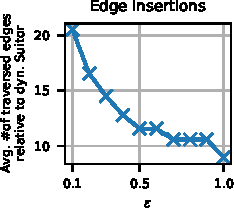
\includegraphics[width=.7\textwidth]{../sources/plots/dyn-mwm/rw-insertion-road-vedges.pdf}
\end{subfigure}\hfill
\begin{subfigure}[t]{.5\textwidth}
\centering
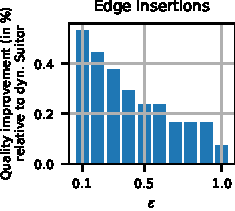
\includegraphics[width=.7\textwidth]{../sources/plots/dyn-mwm/rw-insertion-road-qual.pdf}
\end{subfigure}
\caption*{\footnotesize Average \emph{\#of traversed edges} and \emph{quality} of
\dynmwmrandom relative to dynamic \suitor. Averaged over 15 road networks with
up to 72M edges.}
\end{figure}\pause

$\epsilon = 1$: \dynmwmrandom visits \emph{\vedgesRWInsRoadHighEps more edges}, yields
just \emph{\qualDropRWInsRoadHighEps better} quality.\smallskip

Dynamic \suitor: \emph{\speedRWRemRoadHighEps faster.}

\onslide<2->{
\begin{tikzpicture}[remember picture,overlay]
    \node[circle,minimum size=.5cm] at (current page.center) [
    draw,align=center,anchor=center,xshift=-1.05cm,yshift=-.7cm,red, very thick]
{};
    \node[circle,minimum size=.5cm] at (current page.center) [
    draw,align=center,anchor=center,xshift=4.75cm,yshift=-.7cm,red, very thick]
{};
\end{tikzpicture}
}
\end{frame}

\begin{frame}[t]{Single Updates -- Complex Networks}
\small
Comparison against \dynmwmrandom~\parencite{conf/acda/AngrimanMSU21}.\smallskip

\quad\faHandORight\ $(1 + \epsilon)$-approx., random walks + dynamic programming.

\begin{figure}
\centering
\begin{subfigure}[t]{.5\textwidth}
\centering
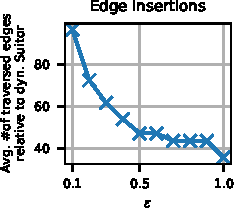
\includegraphics[width=.7\textwidth]{../sources/plots/dyn-mwm/rw-insertion-cplx-vedges.pdf}
\end{subfigure}\hfill
\begin{subfigure}[t]{.5\textwidth}
\centering
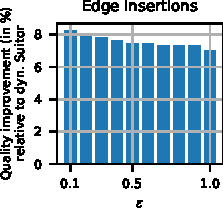
\includegraphics[width=.7\textwidth]{../sources/plots/dyn-mwm/rw-insertion-cplx-qual.pdf}
\end{subfigure}
\caption*{\footnotesize Average \emph{\#of traversed edges} and \emph{quality} of
\dynmwmrandom relative to dynamic \suitor. Averaged over 10 complex networks with
up to 437M edges.}
\end{figure}\pause

$\epsilon = 1$: \dynmwmrandom visits \emph{\vedgesRWInsCplxHighEps more edges}, yields
\emph{\qualDropRWInsCplxHighEps better} quality.\smallskip

Same running time (due to better data structures used by \dynmwmrandom).

\onslide<2->{
\begin{tikzpicture}[remember picture,overlay]
    \node[circle,minimum size=.5cm] at (current page.center) [
    draw,align=center,anchor=center,xshift=-1.05cm,yshift=-.7cm,red, very thick]
{};
    \node[circle,minimum size=.5cm] at (current page.center) [
    draw,align=center,anchor=center,xshift=4.75cm,yshift=1.25cm,red, very thick]
{};
\end{tikzpicture}
}
\end{frame}

%\begin{frame}{Batch Updates}
%\small
%
%\begin{figure}
%\centering
%\begin{subfigure}[b]{.5\textwidth}
%\centering
%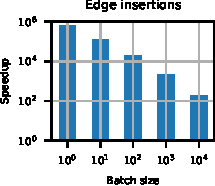
\includegraphics[width=.7\textwidth]{../sources/plots/dyn-mwm/speedup-road-insertion.pdf}
%\caption*{Road networks}
%\end{subfigure}\hfill
%\begin{subfigure}[b]{.5\textwidth}
%\begin{subfigure}[b]{\textwidth}
%\centering
%
\includegraphics{../sources/plots/dyn-mwm/legend-cplx.pdf}
%\end{subfigure}\smallskip
%
%\begin{subfigure}[b]{\textwidth}
%\centering
%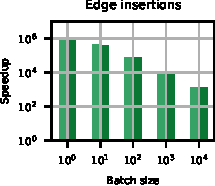
\includegraphics[width=.7\textwidth]{../sources/plots/dyn-mwm/speedup-cplx-insertion.pdf}
%\caption*{Complex networks}
%\end{subfigure}
%\end{subfigure}
%\caption*{\footnotesize Average speedups over a \emph{static recomputation}.}
%\end{figure}\pause
%
%$10^4$ edge insertions: \emph{\speedupRoadInsBTenThou} (road)
%\emph{\speedupCplxInsBTenThouExp} (complex).
%\end{frame}

\subsection{Conclusions}
\begin{frame}{Conclusions -- Dynamic MWM}
\small

\textbf{Dynamic MWM on large graphs}
\begin{itemize}
    \small
    \item Exact computation not feasible
    \item Static approx. too slow
    \item[\faHandORight] Efficient dynamic algorithms\smallskip

        \faExclamationCircle\ Only a few have (recently) been
        implemented~\parencite{conf/acda/AngrimanMSU21}
\end{itemize}\medskip

\textbf{New batch-dynamic \suitor algorithm}
\begin{itemize}
\small
\item Requires \emph{$10\times$} less work (\#of traversed edges) than \dynmwmrandom
\item Yields \emph{$\qualRWRemRoadHighEps$} quality in road networks
    and \emph{$\qualRWRemCplxHighEps$} quality in complex networks
\item Batches with \emph{$10^4$} updates, \emph{$>100\times$} faster than a static
    re-run
\end{itemize}
\end{frame}



%%%%%%%%%%%%%%%%%%%%%%%%%%%%%%%%%%%%%%%%%%%%
% END
%%%%%%%%%%%%%%%%%%%%%%%%%%%%%%%%%%%%%%%%%%%%

\section{Thank You!}
\begin{frame}
\vfill
\begin{center}
\Huge\textbf{\textcolor{HUBblue}{Thank you!}}
\end{center}
\vfill
\scriptsize
Acknowledgments
\begin{itemize}
\scriptsize
\item German Research Foundation (\textbf{DFG}) grant ME 3619/3-2 within
\\ Priority Programme 1736 \textit{Algorithms for Big Data} \item
\textbf{DFG} grant ME 3619/4-1: \\ \textit{Accelerating Matrix
Computations for Mining Large Dynamic Complex Networks} \par
\end{itemize}

\vfill
\end{frame}

\begin{frame}[allowframebreaks]
\frametitle{References}
% This prints the bibliography on the slide
\printbibliography
\end{frame}
% AT END: Summary of all results

\ifbackup
\section{Backup Slides}

\subsection{Top-$k$ Closeness}

\begin{frame}[t]{Dynamic Top-$k$ Closeness}
\framesubtitle{Affected Vertices}

\tiny\centering
\setlength{\tabcolsep}{3pt}
\begin{tabular}{lrrrrr|rrrr}
\toprule
Network & \multirow{2}{*}{Aff.} & \multirow{2}{*}{Aff. (\%)} &\multirow{2}{*}{F (\%)} & \multirow{2}{*}{B (\%)} & \multirow{2}{*}{D (\%)} & \multicolumn{3}{c}{BFScuts (\%)} \\
Batch size & & & & & & 1 & 10 & 100 \\
\midrule
petster-cat-household & \numprint{3505} & \numprint{3.33} & \numprint{99.45} & \numprint{0.32} & \numprint{0.23} & $<\numprint{0.01}$ & \numprint{0.03} & \numprint{0.22}\\
petster-catdog-household & \numprint{14518} & \numprint{4.36} & \numprint{89.09} & \numprint{10.68} & \numprint{0.23} & $<\numprint{0.01}$ & \numprint{0.04} & \numprint{0.22}\\
petster-cat-friend & \numprint{26} & \numprint{0.01} & \numprint{84.69} & \numprint{14.16} & \numprint{1.15} & $<\numprint{0.01}$ & $<\numprint{0.01}$ & $<\numprint{0.01}$\\
petster-friendships-cat & \numprint{30} & \numprint{0.02} & \numprint{86.89} & \numprint{12.07} & \numprint{1.05} & $<\numprint{0.01}$ & $<\numprint{0.01}$ & $<\numprint{0.01}$\\
petster-friendships-dog & \numprint{1440} & \numprint{0.34} & \numprint{88.76} & \numprint{9.58} & \numprint{1.66} & $<\numprint{0.01}$ & \numprint{0.01} & \numprint{0.17}\\
petster-dog-friend & \numprint{446} & \numprint{0.10} & \numprint{24.59} & \numprint{66.61} & \numprint{8.80} & $<\numprint{0.01}$ & \numprint{0.02} & \numprint{0.17}\\
petster-catdog-friend & \numprint{1620} & \numprint{0.26} & \numprint{92.43} & \numprint{6.37} & \numprint{1.20} & $<\numprint{0.01}$ & $<\numprint{0.01}$ & \numprint{0.15}\\
higgs-twitter-social & \numprint{10342} & \numprint{2.26} & \numprint{84.54} & \numprint{13.59} & \numprint{1.87} & $<\numprint{0.01}$ & \numprint{0.08} & \numprint{1.05}\\
petster-carnivore & \numprint{269} & \numprint{0.04} & \numprint{66.75} & \numprint{27.55} & \numprint{5.70} & $<\numprint{0.01}$ & \numprint{0.02} & \numprint{0.18}\\
\bottomrule
\end{tabular}
\smallskip

\begin{tabular}{lrrrrr|rrrr}
\toprule
Network & \multirow{2}{*}{Aff.} & \multirow{2}{*}{Aff. (\%)} &\multirow{2}{*}{F (\%)} & \multirow{2}{*}{B (\%)} & \multirow{2}{*}{D (\%)} & \multicolumn{3}{c}{BFScuts (\%)} \\
Batch size & & & & & & 1 & 10 & 100 \\
\midrule
wikipedia\_link\_li & \numprint{2531} & \numprint{5.15} & \numprint{0.10} & \numprint{0.30} & \numprint{99.60} & \numprint{3.51} & \numprint{32.53} & \numprint{94.26}\\
cit-HepPh & \numprint{615} & \numprint{1.78} & \numprint{65.31} & \numprint{4.97} & \numprint{29.73} & \numprint{0.37} & \numprint{3.66} & \numprint{29.08}\\
slashdot-zoo & \numprint{1888} & \numprint{2.39} & \numprint{51.99} & \numprint{11.59} & \numprint{36.43} & \numprint{0.53} & \numprint{7.53} & \numprint{41.64}\\
wiki\_talk\_sv & \numprint{1397} & \numprint{0.23} & \numprint{94.37} & \numprint{5.27} & \numprint{0.36} & $<\numprint{0.01}$ & \numprint{1.16} & \numprint{5.31}\\
munmun\_twitter\_social & \numprint{139} & \numprint{0.03} & \numprint{47.80} & \numprint{20.74} & \numprint{31.46} & $<\numprint{0.01}$ & $<\numprint{0.01}$ & \numprint{0.04}\\
wiki\_talk\_ja & \numprint{1475} & \numprint{0.14} & \numprint{15.98} & \numprint{18.33} & \numprint{65.68} & \numprint{0.05} & \numprint{0.47} & \numprint{2.61}\\
wikipedia\_link\_gu & \numprint{191} & \numprint{0.63} & \numprint{11.43} & \numprint{12.11} & \numprint{76.46} & \numprint{0.47} & \numprint{4.73} & \numprint{25.54}\\
web-NotreDame & \numprint{6332} & \numprint{1.94} & \numprint{91.81} & \numprint{3.33} & \numprint{4.86} & \numprint{0.08} & \numprint{0.36} & \numprint{3.74}\\
digg-friends & \numprint{708} & \numprint{0.02} & \numprint{66.00} & \numprint{18.05} & \numprint{15.95} & $<\numprint{0.01}$ & \numprint{0.03} & \numprint{0.26}\\
\bottomrule
\end{tabular}

\end{frame}

\begin{frame}[t]{Dynamic Top-$k$ Closeness}
\framesubtitle{Speedups}\vspace{-1cm}

\begin{figure}
\centering
\begin{subfigure}[t]{\textwidth}
\centering
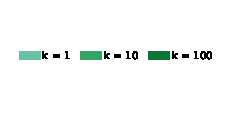
\includegraphics{../sources/plots/dyn-topk/legend-speedup.pdf}
\end{subfigure}\vspace{-1cm}

\begin{subfigure}[t]{\textwidth}
\begin{subfigure}[t]{.5\textwidth}
\caption*{\scriptsize Complex networks}
\begin{subfigure}[t]{.5\textwidth}
\centering
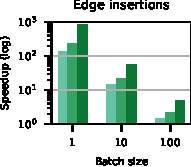
\includegraphics[width=.9\textwidth]{../sources/plots/dyn-topk/speedup-undirected-small-diameter-addition.pdf}
\end{subfigure}\hfill
\begin{subfigure}[t]{.5\textwidth}
\centering
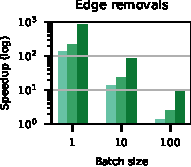
\includegraphics[width=.9\textwidth]{../sources/plots/dyn-topk/speedup-undirected-small-diameter-removal.pdf}
\end{subfigure}
\end{subfigure}\hfill
\begin{subfigure}[t]{.5\textwidth}
\caption*{\scriptsize Road networks}
\begin{subfigure}[t]{.5\textwidth}
\centering
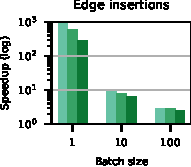
\includegraphics[width=.9\textwidth]{../sources/plots/dyn-topk/speedup-undirected-high-diameter-addition.pdf}
\end{subfigure}\hfill
\begin{subfigure}[t]{.5\textwidth}
\centering
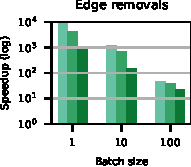
\includegraphics[width=.9\textwidth]{../sources/plots/dyn-topk/speedup-undirected-high-diameter-removal.pdf}
\end{subfigure}
\end{subfigure}
\end{subfigure}
\end{figure}

\begin{minipage}[t]{.4\textwidth}
\scriptsize
\hfill Results for $k = 10$
\end{minipage}\hfill
\begin{minipage}[t]{.6\textwidth}
\scriptsize\centering
\setlength{\tabcolsep}{3pt}
\begin{tabular}{lrr|rr}
\toprule
\multirow{2}{*}{Network} & \multirow{2}{*}{$n$} & \multirow{2}{*}{$m$} & \multicolumn{2}{c}{Batch size 10} \\
                         & & & Static (s) & Dyn. (s) \\
\midrule
\vdots &\vdots &\vdots & \vdots & \vdots\\
twitter & 456K & 14.8M & \numprint{163.5} & \numprint{3.8} \\
petster & 623K & 15.6M & \numprint{1845.4} & \numprint{3.4} \\
\bottomrule
\end{tabular}
\end{minipage}
\end{frame}


\subsection{Betweenness Centrality}

\begin{frame}[t]{Betweenness Centrality}
\scriptsize
\begin{minipage}[t]{.5\textwidth}
\vspace{-5mm}
\begin{block}{\scriptsize\kadabra~\parencite{DBLP:conf/esa/BorassiN16}: Adaptive Sampling}
\begin{itemize}
    \scriptsize
\item[\faHandORight] \# of samples is not fixed
\item[\faHandORight] \emph{stopping condition} depends on sampled data
\end{itemize}
\end{block}

\begin{algorithmic}[1]
\Repeat
\State$\mathit{agg} \gets \mathit{agg} \circ \Call{sample}{ }$
\Until{$\Call{checkStop}{\mathit{agg}}$}
\end{algorithmic}\medskip

\faExclamationCircle\ $\Call{sample}{}$ and $\Call{checkStop}{}$ are \emph{inherently sequential}.

\faExclamationCircle\ The algorithm needs to be \emph{serializable}.\smallskip

\textbf{Challenge:} parallelize adaptive sampling.
\end{minipage}\hfill
\begin{minipage}[t]{.45\textwidth}
\textbf{Solution:} epoch-based algorithm~\parencite{DBLP:conf/europar/GrintenAM19}.

\begin{tikzpicture}[scale=.5,boxstyle/.style={
    draw,rectangle,minimum height=.4cm,align=center,font=\scriptsize,
}]
    \node[] at (0,0) (t1) {\scriptsize T1};
    \node[below=.3cm of t1] (t2) {\scriptsize T2};
    \node[below=.3cm of t2] (t3) {\scriptsize T3};
    \node[below=.3cm of t3] (t4) {\scriptsize T4};

    \node[above right=.5cm and -.2cm of t1] (time1) {};
    \node[above right=.5cm and 5cm of t1] (time2) {};
    \node[above right=.75cm and 0cm of t1] {\scriptsize time};
    \draw[->,thick] (time1) to (time2);

    \node[boxstyle,minimum width=1cm, right=.1cm of t1] (e11) {1};
    \node[boxstyle,minimum width=2cm, right=.1cm of t2] (e21) {1};
    \node[boxstyle,minimum width=.5cm, right=.1cm of t3] (e31) {1};
    \node[boxstyle,minimum width=.75cm, right=.1cm of t4] (e41) {1};
    \node[boxstyle,minimum width=1.2cm, right=.1cm of e11] (e12) {2};
    \node[boxstyle,minimum width=.8cm, right=.1cm of e21] (e22) {2};
    \node[boxstyle,minimum width=2.1cm, right=.1cm of e31] (e32) {2};
    \node[boxstyle,minimum width=1.1cm, right=.1cm of e41] (e42) {2};
    \node[right=.1cm of e12] (d1) {\dots};
    \node[right=.1cm of e22] (d2) {\dots};
    \node[right=.1cm of e32] (d3) {\dots};
    \node[right=.1cm of e42] (d4) {\dots};

    \node[boxstyle,minimum width=1.5cm, right=.2 of d1] (f1) {k+1};
    \node[boxstyle,minimum width=1.4cm, right=.2 of d2] (f2) {k+1};
    \node[boxstyle,minimum width=1.7cm, right=.2 of d3] (f3) {k+1};
    \node[boxstyle,minimum width=1.4cm, right=.2 of d4] (f4) {k};

    \node[below right= .1cm and -.1cm of f4] (dash_bottom) {};
    \node[above right= 2.5cm and -.1cm of f4] (dash_top) {};
    \node[below left=-.1cm and 0cm of dash_bottom] () {\scriptsize\emph{$\Call{checkStop}{\mathit{agg}$} = \texttt{true}}};
    \draw[dashed,thick,\emphcolor] (dash_bottom) to (dash_top);

\end{tikzpicture}
\end{minipage}

\begin{minipage}[t]{.5\textwidth}
\begin{figure}
\centering
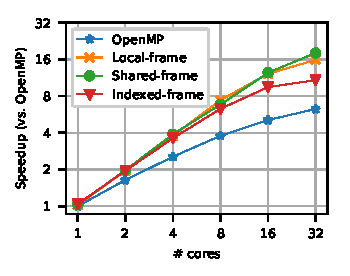
\includegraphics[width=.65\textwidth]{../sources/plots/betw-apx/parallel-speedup.pdf}
\end{figure}
%\centering
%\begin{itemize}
%    \scriptsize
%\item[\faThumbsOUp] Good parallel scalability
%\item[\faThumbsOUp] On 32 cores: $3\times$ faster than straightforward OpenMP parallelization
%\end{itemize}
%\vspace{-3mm}
\end{minipage}\hfill
\begin{minipage}[t]{.5\textwidth}
\centering\vspace{2mm}

\begin{table}
\setlength{\tabcolsep}{3pt}
\scriptsize
\begin{tabular}{lrrrr}
\toprule
\multirow{2}{*}{Network} & \multirow{2}{*}{$n$} & \multirow{2}{*}{$m$} & \multicolumn{2}{c}{Time (s) on 32 cores} \\
 & & & OpenMP & Epoch-Based\\
\midrule
wiki\_sr & 3.2M & 103.3M & 13 & 3 \\
orkut & 3.1M & 117.2M & 15 & 7\\
\bottomrule
\end{tabular}
\caption*{\scriptsize Results for $\epsilon = \numprint{0.01}$}
\end{table}
\end{minipage}
\end{frame}

\begin{frame}[t]{Betweenness Centrality}
\begin{minipage}[t]{.5\textwidth}
\centering
\begin{figure}
\centering
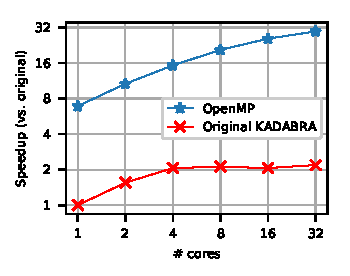
\includegraphics[width=.7\textwidth]{../sources/plots/betw-apx/original-vs-baseline.pdf}
\caption*{\scriptsize Average speedup of OpenMP baseline over
the original sequential implementation of \kadabra.}
\end{figure}
\end{minipage}\hfill
\begin{minipage}[t]{.5\textwidth}
\begin{figure}
\centering
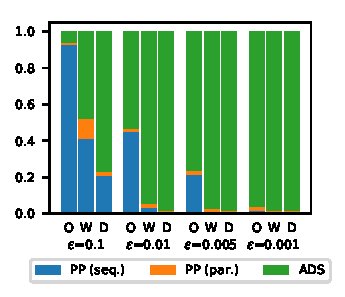
\includegraphics[width=.7\textwidth]{../sources/plots/betw-apx/time-breakdown.pdf}
\caption*{\scriptsize Breakdown of sequential \kadabra running times into preprocessing and ADS
(in percent).}
\end{figure}
\end{minipage}
\end{frame}


\subsection{Electrical Closeness}

\begin{frame}[t]{Electrical Closeness}
\footnotesize
%Electrical closeness: $\elclos(u) := \frac{n - 1}{\sum_{v \in V} \rdist(u, v)}$.\smallskip
%
%Sota: JLT + fast Laplacian solvers $\Rightarrow$ solve $\Oh(\log n / \epsilon^2)$ Laplacian systems, $(1 + \epsilon)$-approx.

\begin{block}{\footnotesize Main idea}
\begin{itemize}
\footnotesize

\item[\faHandORight] Only $\diag{\Linv}$ is necessary to compute
$\elclos(\cdot)$~\parencite{DBLP:journals/socnet/BozzoF13}.%:
%$\sum_{v \in V} \rdist(u, v) := n\cdot\Linv[u,u] + \tr{\Linv}$.

\item[\faHandORight] Solve one linear system $\Lapl\vect{x} = \cunit{u} - \frac{1}{n}\cdot\ones\ \leadsto\ \emph{\Linv[:, u]}$.

\item[\faHandORight] Remaining $n-1$ diagonal entries: $\Linv[v,v] = \emph{\rdist(u, v)} - \Linv[u, u] + 2\Linv[v, u]$.\\

via \emph{UST sampling}~\parencite{DBLP:conf/esa/AngrimanPGM20}.
\end{itemize}
\end{block}\vspace{-5mm}

\begin{minipage}[t]{.48\textwidth}
\begin{block}{\footnotesize\textbf{Theorem}}
    Current flowing through an edge $e = (a, b)$:
    $$i(a, b) = (N_{s, t}(a, b) - N_{s, t}(b, a)) / N$$
\end{block}
\end{minipage}\hfill
\begin{minipage}[t]{.48\textwidth}
\begin{block}{\footnotesize Idea}
Compute $\rdist(u, v)$ by adding the currents on a path from $u$ to $v$.
\end{block}
\end{minipage}

\begin{minipage}[t]{.5\textwidth}
\footnotesize\medskip

Compared to competitors:
\begin{itemize}
    \footnotesize
\item[\faThumbsOUp] Better approximation of $\diag{\Linv}$
    \begin{itemize}
    \scriptsize
        \item absolute error
        \item full vertex ranking
    \end{itemize}
\item[\faThumbsOUp] $10\times$ faster
\end{itemize}
\end{minipage}\hfill
\begin{minipage}[t]{.5\textwidth}
    \centering\vspace*{1mm}\scriptsize

\begin{table}
\setlength{\tabcolsep}{3pt}
\begin{tabular}{lrr|rr}
\toprule
\multirow{2}{*}{Network} & \multirow{2}{*}{$n$} & \multirow{2}{*}{$m$} & \multicolumn{2}{c}{Time (s)} \\
& & & $\epsilon = 0.3$ & $\epsilon = 0.9$ \\
\midrule
orkut & \numprint{3.1}M & \numprint{117.2}M & \numprint{71.8} & \numprint{19.9}\\
wiki\_en & \numprint{13.6}M & \numprint{334.6}M & \numprint{429.9} & \numprint{88.3}\\
\bottomrule
\end{tabular}
\caption*{\scriptsize Running time on $16\times 24$ cores.}
\end{table}
\end{minipage}
\end{frame}

\begin{frame}[t]{Electrical Closeness}
\begin{figure}
\begin{subfigure}[t]{.33\textwidth}
\centering
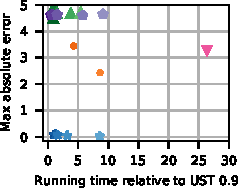
\includegraphics[width=.9\textwidth]{../sources/plots/el-clos/abs-errors.pdf}
\end{subfigure}\hfill
\begin{subfigure}[t]{.33\textwidth}
\centering
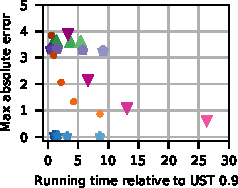
\includegraphics[width=.9\textwidth]{../sources/plots/el-clos/avg-abs-errors.pdf}
\end{subfigure}\hfill
\begin{subfigure}[t]{.33\textwidth}
\centering
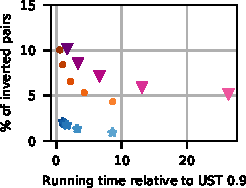
\includegraphics[width=.9\textwidth]{../sources/plots/el-clos/full-ranking.pdf}
\end{subfigure}

\begin{subfigure}[t]{\textwidth}
\centering
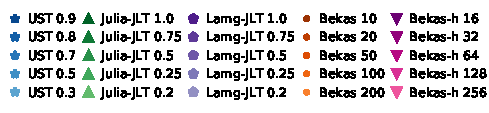
\includegraphics[width=.45\textwidth]{../sources/plots/el-clos/legend-quality.pdf}
\end{subfigure}\bigskip

\begin{subfigure}[t]{\textwidth}
\centering
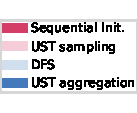
\includegraphics[width=.15\textwidth]{../sources/plots/el-clos/legend-time-breakdown.pdf}
\hspace{2mm}
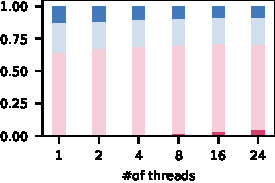
\includegraphics[width=.35\textwidth]{../sources/plots/el-clos/time-breakdown.pdf}
\end{subfigure}
\end{figure}
\end{frame}


\begin{frame}[t]{Forest Closeness}
\centering
\begin{figure}
\begin{subfigure}[t]{\textwidth}
\centering
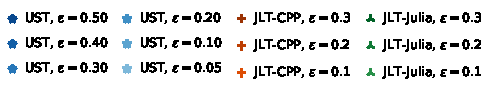
\includegraphics[width=.4\textwidth]{../sources/plots/el-clos/forest-quality-legend.pdf}
\end{subfigure}

\begin{subfigure}[t]{.5\textwidth}
\centering
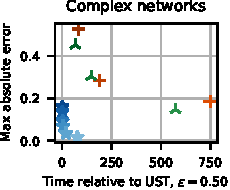
\includegraphics[width=.6\textwidth]{../sources/plots/el-clos/forest-max-abs-err-cplx.pdf}
\end{subfigure}\hfill
\begin{subfigure}[t]{.5\textwidth}
\centering
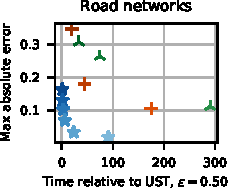
\includegraphics[width=.6\textwidth]{../sources/plots/el-clos/forest-max-abs-err-road.pdf}
\end{subfigure}\smallskip

\begin{subfigure}[t]{.5\textwidth}
\centering
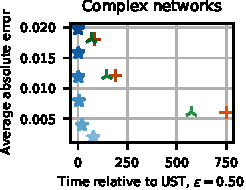
\includegraphics[width=.6\textwidth]{../sources/plots/el-clos/avg-abs-small-diam-unweighted.pdf}
\end{subfigure}\hfill
\begin{subfigure}[t]{.5\textwidth}
\centering
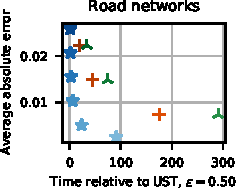
\includegraphics[width=.6\textwidth]{../sources/plots/el-clos/avg-abs-high-diam-unweighted.pdf}
\end{subfigure}
\end{figure}
\end{frame}


\begin{frame}[t]{Group Forest Closeness}
\begin{figure}
\begin{subfigure}[t]{\textwidth}
\centering

\includegraphics[width=.4\textwidth]{../sources/plots/el-clos/legend-node-class.pdf}
\end{subfigure}

\begin{subfigure}[t]{.5\textwidth}
\centering
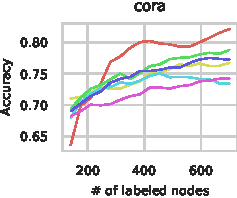
\includegraphics[width=.6\textwidth]{../sources/plots/el-clos/node-class-cora.pdf}
\end{subfigure}\hfill
\begin{subfigure}[t]{.5\textwidth}
\centering
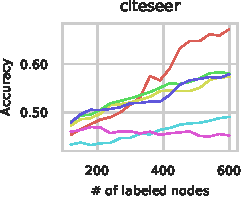
\includegraphics[width=.6\textwidth]{../sources/plots/el-clos/node-class-citeseer.pdf}
\end{subfigure}\smallskip

\begin{subfigure}[t]{.5\textwidth}
\centering
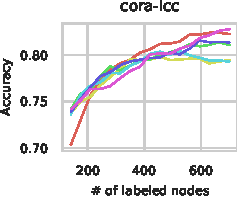
\includegraphics[width=.6\textwidth]{../sources/plots/el-clos/node-class-cora_lcc.pdf}
\end{subfigure}\hfill
\begin{subfigure}[t]{.5\textwidth}
\centering
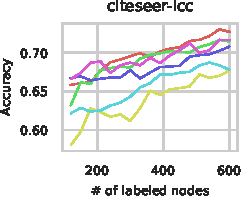
\includegraphics[width=.6\textwidth]{../sources/plots/el-clos/node-class-citeseer_lcc.pdf}
\end{subfigure}
\end{figure}
\end{frame}

\subsection{Grow-Shrink -- Backward Edges}
\begin{frame}{Grow-Shrink -- Far Vertices}
\small
Limitation of lower bound for $\deltafarnm(v)$ for vertices $v$ far from $S$:

\begin{figure}[H]
\begingroup\centering
\begin{tikzpicture}[scale=.8]
\drawgraphcontour
\drawgroupcontour

\simplenode{\nodeida}{\coorda}
\simplenode{\nodeidb}{\coordb}
\simplenode{\nodeidc}{\coordc}
\simplenode{\nodeidd}{\coordd}
\simplenode{\nodeide}{\coorde}
\simplenode{\nodeidf}{\coordf}

\simplenode{\nodeidg}{\coordg}
\customcolornode{\nodeidh}{\coordh}{red}
\simplenode{\nodeidi}{\coordi}
\simplenode{\nodeidj}{\coordj}

\simplenode{\nodeidk}{\coordk}
\customcolornode{\nodeidl}{\coordl}{red}
\node[] at ([yshift=.4cm]\coordn) {$v$};
\customcolornode{\nodeidm}{\coordm}{red}
\customcolornode{\nodeidn}{\coordn}{cyan}
\simplenode{\nodeido}{\coordo}

\customcolornode{\nodeidp}{\coordp}{red}
\customcolornode{\nodeidq}{\coordq}{cyan}
\customcolornode{\nodeidr}{\coordr}{cyan}

\node[align=left] at (12, .25) {\textnormal{Forward contrib.}};
\node[align=left] at (12, -.25) {\textnormal{Backward contrib.}};
\node[align=left] at (10, -2) {\normalsize$\deltafarnm(v) \ge |\textcolor{cyan}{D_v}|\cdot d(S, v)$};

\coordinate[] (f1) at (9.5, .25);
\coordinate[] (f2) at (10.25, .25);
\coordinate[] (b1) at (9.5, -.25);
\coordinate[] (b2) at (10.25, -.25);
\draw[thick,cyan] (f1) -- (f2);
\draw[thick,red] (b1) -- (b2);

\edgecoords

\draw[->] (sg1) -- (ng3);
\draw[->] (sg11) -- (ng21);
\draw[->] (sg2) -- (ng4);
\draw[->] (sg3) -- (ng2);
\draw[->] (sg4) -- (ng1);
\draw[<-] (sg5) -- (sg3b);
\draw[<-] (sg6) -- (sg2b);

\draw[->] (ng1b) -- (ng5);
\draw[->,red,thick] (ng2b2) -- (ng6);
\draw[->,red,thick] (ng2b) -- (ng7);
\draw[->,red,thick] (ng2b1) -- (ng81);
\draw[->] (ng3b) -- (ng8);
\draw[->] (ng3b1) -- (ng9);

\draw[->,red,thick] (ng6b) -- (ng10);
\draw[->,cyan,thick] (ng7b) -- (ng11);
\draw[->,cyan,thick] (ng7b1) -- (ng12);

\end{tikzpicture}
\endgroup\par

\end{figure}
\end{frame}

\subsection{Group-Closeness -- Local-Swaps}

\begin{frame}{Local-Swaps}
\framesubtitle{For \emph{unweighted} graphs}
%
\vspace{3mm}
\textbf{Local approach:}
\begin{itemize}
    \item Only allow swaps between vertices in $S$ and their \emph{neighbors}
    \item After each swap: \[\forall x\in V\quad\left(d(S, x) - d(\Suv, x) \right)\in \{-1, 0, +1\}\]
\end{itemize}

\vspace{-4mm}
\begingroup\centering
\begin{tikzpicture}[scale=.9]
\tikzstyle{every node}=[font=\itshape,inner sep=0, minimum size=.3cm, outer sep=0]

\drawgraphcontour
\drawswapgroupcontour

\simplenode{\nodeida}{\coorda}
\simplenode{\nodeidb}{\coordb}
\simplenode{\nodeidd}{\coordd}
\simplenode{\nodeidf}{\coordf}
\simplenode{\nodeidg}{\coordg}

\customcolornode{\nodeidc}{\coordc}{magenta}
\customcolornode{\nodeide}{\coorde}{magenta}
\customcolornode{\nodeidh}{\coordh}{cyan}
\customcolornode{\nodeidl}{\coordl}{cyan}
\customcolornode{\nodeidm}{\coordm}{cyan}
\customcolornode{\nodeidn}{\coordn}{cyan}
\customcolornode{\nodeidp}{\coordp}{cyan}
\customcolornode{\nodeidq}{\coordq}{cyan}
\customcolornode{\nodeidr}{\coordr}{cyan}

\node[magenta] at ([xshift=-2pt,yshift=10pt]\coordc) {$+1$};
\node[magenta] at ([yshift=-10pt]\coorde) {$+1$};

\node[cyan] at ([yshift=-10pt]\coordh) {$-1$};
\node[cyan] at ([yshift=10pt]\coordl) {$-1$};
\node[cyan] at ([yshift=-10pt]\coordm) {$-1$};
\node[cyan] at ([yshift=-10pt]\coordn) {$-1$};
\node[cyan] at ([yshift=10pt]\coordp) {$-1$};
\node[cyan] at ([xshift=15pt]\coordq) {$-1$};
\node[cyan] at ([yshift=-10pt]\coordr) {$-1$};

    \node[] at (9, -1.5) {\textnormal{Here:}};
    \node[] at (9, -2.3) {$f(S) - f(\Suv) = \textcolor{cyan}{7} - \textcolor{magenta}{2} = 5$};

\simplenode{\nodeidi}{\coordi}
\simplenode{\nodeidj}{\coordj}

\simplenode{\nodeidk}{\coordk}
\simplenode{\nodeido}{\coordo}

\edgecoords

\draw[->] (sg1) -- (ng3);
\draw[->] (sg11) -- (ng21);
\draw[->] (sg2) -- (ng4);
\draw[->] (sg4) -- (ng1);
\draw[<-] (sg6) -- (sg2b);
\draw[<-] (sg5) -- (sg3b);
\draw[<-] (sg3) -- (ng2);

\draw[->] (ng1b) -- (ng5);
\draw[->] (ng2b2) -- (ng6);
\draw[->] (ng2b) -- (ng7);
\draw[->] (ng2b1) -- (ng81);
\draw[->] (ng3b) -- (ng8);
\draw[->] (ng3b1) -- (ng9);

\draw[->] (ng6b) -- (ng10);
\draw[->] (ng7b) -- (ng11);
\draw[->] (ng7b1) -- (ng12);
\end{tikzpicture}
\endgroup\par


\end{frame}


\begin{frame}{Local-Swaps -- {\LARGE Computing $\gfarn(S) - \gfarn(\Suv)$}}
\medskip\footnotesize

Dynamic data structures:\medskip

\begin{itemize}
    \footnotesize
    \newcommand{\lambdaw}{$\Lambda_z := \{x \in \overline{S} : \lambda_x = \{z\}\}$ for all $z\in S$}
    \item Distance $d(S, x)$ from $S$ to all $x \in \overline{S}$\smallskip
    \item Set $\lambda_x := \{z \in S : d(S, x) = d(z, x)\}$ for all $x\in \overline{S}$\smallskip
    \item\textcolor{HUBmagenta}{\lambdaw}
\end{itemize}\bigskip

\begin{minipage}[t]{.5\textwidth}
Good $(u,v)$ swap: maximize
$\textcolor{cyan}{|D_v|} - \textcolor{magenta}{|\Lambda_u|}$
\begin{enumerate}
    \footnotesize
    \item Find $v\in N(S)\setminus S$ that maximizes \textcolor{cyan}{$|D_v|$}
    \item Find $u \in N(v)\cap S$ that minimizes \textcolor{magenta}{$|\Lambda_u|$}
\end{enumerate}
\end{minipage}\hfill
\begin{minipage}[t]{.4\textwidth}
\begin{figure}
\centering
\hspace{-1cm}\begingroup\centering
\begin{tikzpicture}[scale=.6]
\renewcommand{\nshift}{6.5pt}

\graphcoords
\graphcontour
\drawswapgroupcontour

\simplenode{\nodeida}{\coorda}
\simplenode{\nodeidb}{\coordb}
\simplenode{\nodeidd}{\coordd}
\simplenode{\nodeidf}{\coordf}
\simplenode{\nodeidg}{\coordg}

\customcolornode{\nodeidc}{\coordc}{magenta}
\customcolornode{\nodeide}{\coorde}{magenta}
\customcolornode{\nodeidh}{\coordh}{cyan}
\customcolornode{\nodeidl}{\coordl}{cyan}
\customcolornode{\nodeidm}{\coordm}{cyan}
\customcolornode{\nodeidn}{\coordn}{cyan}
\customcolornode{\nodeidp}{\coordp}{cyan}
\customcolornode{\nodeidq}{\coordq}{cyan}
\customcolornode{\nodeidr}{\coordr}{cyan}

\newcommand{\plone}{\scriptsize$+1$}
\newcommand{\mione}{\scriptsize$-1$}

\node[magenta] at ([xshift=-2pt,yshift=11pt]\coordc) {\plone};
\node[magenta] at ([yshift=-11pt]\coorde) {\plone};

\node[cyan] at ([yshift=-11pt]\coordh) {\mione};
\node[cyan] at ([yshift=11pt]\coordl) {\mione};
\node[cyan] at ([yshift=-11pt]\coordm) {\mione};
\node[cyan] at ([yshift=-11pt]\coordn) {\mione};
\node[cyan] at ([yshift=11pt]\coordp) {\mione};
\node[cyan] at ([xshift=15pt]\coordq) {\mione};
\node[cyan] at ([yshift=-11pt]\coordr) {\mione};

\simplenode{\nodeidi}{\coordi}
\simplenode{\nodeidj}{\coordj}

\simplenode{\nodeidk}{\coordk}
\simplenode{\nodeido}{\coordo}

\edgecoords

\draw[->] (sg1) -- (ng3);
\draw[->] (sg11) -- (ng21);
\draw[->] (sg2) -- (ng4);
\draw[<-] (sg3) -- (ng2);
\draw[->] (sg4) -- (ng1);
\draw[<-] (sg5) -- (sg3b);
\draw[<-] (sg6) -- (sg2b);

\draw[->] (ng1b) -- (ng5);
\draw[->] (ng2b2) -- (ng6);
\draw[->] (ng2b) -- (ng7);
\draw[->] (ng2b1) -- (ng81);
\draw[->] (ng3b) -- (ng8);
\draw[->] (ng3b1) -- (ng9);

\draw[->] (ng6b) -- (ng10);
\draw[->] (ng7b) -- (ng11);
\draw[->] (ng7b1) -- (ng12);
\end{tikzpicture}
\endgroup\par


\end{figure}
\end{minipage}\medskip

\begin{block}{\centering\textcolor{black}{$\gfarn(S) - \gfarn(\Suv) =
\textcolor{cyan}{|H^-_{u, v}|} - \textcolor{magenta}{|H^+_{u, v}|}$}}
\vspace{-3ex}
\end{block}
\end{frame}

\subsection{Group-Closeness -- Number of Exchanges}

\begin{frame}[t]{\growshrink\ -- Number of Exchanges}

\begin{figure}
\centering
\begin{subfigure}[t]{.8\textwidth}
\centering
\includegraphics{../sources/plots/local-search-heu/legend-unweighted.pdf}
\end{subfigure}\smallskip

\begin{subfigure}[t]{.5\textwidth}
\centering
\includegraphics[width=.7\textwidth]{../sources/plots/local-search-heu/impact-num-exchanges-unweighted.pdf}
\caption*{\scriptsize Unweighted graphs}
\end{subfigure}\hfill
\begin{subfigure}[t]{.5\textwidth}
\centering
\includegraphics[width=.7\textwidth]{../sources/plots/local-search-heu/impact-num-exchanges-weighted.pdf}
\caption*{\scriptsize Weighted graphs}
\end{subfigure}
\caption*{\footnotesize Group-closeness score relative to greedy depending on the number of vertex exchanges
(results for $k = 10$).}
\end{figure}
\end{frame}


\subsection{Group-Closeness Approximation}

\begin{frame}[t]{Group-Closeness Approximation}
\footnotesize
Group-closeness maximization $\longleftrightarrow$ \emph{metric $k$-Median} problem:\medskip

\begin{minipage}[t]{.45\textwidth}
\textbf{Input:}
\begin{itemize}
    \scriptsize
    \item sets of clients $C$ and facilities $F$
    \item cost function $f: C\times F \to \mathbb{R}_{\ge 0}$
    \item integer $k$
\end{itemize}\smallskip

\scriptsize
\textbf{Find:} $S^\star := \argmin_{\substack{S\subset F\\|S| \le k}}\sum_{i\in C}\min_{j\in F}f(i,j)$
\end{minipage}\hfill
\begin{minipage}[t]{.55\textwidth}
    \textbf{Approximation algorithm}~\parencite{DBLP:journals/siamcomp/AryaGKMMP04}:
\begin{itemize}
\scriptsize
\item Based on local search
\item $(1 + \frac{1}{e})$-approximation for metric $k$-Median~\parencite{DBLP:journals/tmc/DAngeloDNP16}
\item[\emph{\faHandORight}] $\frac{e}{(e + 1)}$-approximation for group-closeness (undirected)
\item[\emph{\faHandORight}] $4\cdot n^{-\epsilon}$ group-closeness
(directed)~\parencite{DBLP:conf/alenex/AngrimanBDGGM21}
\end{itemize}
\end{minipage}\bigskip

\begin{minipage}[t]{.55\textwidth}
\begin{figure}
\begin{subfigure}[t]{\textwidth}
\centering
\includegraphics[width=.7\textwidth]{../sources/plots/gh-gc-apx/legend-quality-closeness.pdf}
\end{subfigure}\smallskip

\begin{subfigure}[t]{.5\textwidth}
\centering
\includegraphics[width=.9\textwidth]{../sources/plots/gh-gc-apx/quality-high-diameter-directed-weighted.pdf}
\end{subfigure}\hfill
\begin{subfigure}[t]{.5\textwidth}
\centering
\includegraphics[width=.9\textwidth]{../sources/plots/gh-gc-apx/quality-high-diameter-undirected-weighted.pdf}
\end{subfigure}
\caption*{\scriptsize Fig.: Group-closeness scores relative to the best over 100 random groups.}
\end{figure}
\end{minipage}\hfill
\begin{minipage}[t]{.4\textwidth}
\scriptsize
Our new local search algorithm (\textsc{LS-C}):
\begin{itemize}
\scriptsize
\item[\faThumbsOUp] Always yields the best quality
\item[\faThumbsODown] $10\times$ to $100\times$ slower than heuristics
\end{itemize}\bigskip

\faHandORight\ Time vs quality trade-off\smallskip

\faHandORight\ Approximation viable only in networks with moderate size
\end{minipage}
\end{frame}


\subsection{GED-Walk}
\begin{frame}[t]{GED-Walk -- Scalable Group Centrality}
\small\smallskip

\begin{minipage}[t]{.45\textwidth}
Popular group centrality measures:
\begin{itemize}
\small
\item based on \emph{distance}
\item \emph{expensive} to optimize
\end{itemize}

\end{minipage}\hfill
\begin{minipage}[t]{.5\textwidth}
\emph{GED-Walk:} new measure~\parencite{DBLP:conf/alenex/AngrimanGBZGM20}
 based on \emph{walks}
%\begin{itemize}
%    \footnotesize
%\item[\faThumbsOUp] \emph{$10\times$} to \emph{$100\times$ faster} to maximize than GBC, GCC and GHC
%    for small groups
%\item[\faThumbsOUp] Allows to analyze graphs with \emph{$>100$M edges in $<30$ min.}
%\item[\faThumbsOUp] Improves quality of semi-supervised vertex classification and
%    graph classification
%\end{itemize}
\end{minipage}

\begin{block}{Definition (Group Exponentially Decaying Walk)}
\small
GED-Walk of $S \subseteq V$:
\[\ged(S) := \sum_{i = 1}^\infty\alpha^i\phi_i(S),\]
\vspace{-4mm}
\begin{itemize}
    \item $\alpha > 0$ controls the importance of long walks
    \item $\phi_i$(S): \#of $i$-walks with at least a vertex in $S$.
\end{itemize}
\end{block}

\begin{itemize}
    \small
    \item Monotone and submodular
    \item $\ged(S) < \infty$ for a \enquote{small enough} $\alpha$
\end{itemize}
\end{frame}

\subsection{GED-Walk -- Separation}

\begin{frame}{GED-Walk -- Separation}

\textbf{Need:} find the top-1 vertex with highest marginal gain.\smallskip

\faHandORight\ Decide if the top-1 node is \enquote{separated} from the others.
\medskip

\bigskip\begingroup\centering
\begin{tikzpicture}
    \node at (0, 0) {$x$};
    \node at (0, -.5) {$y$};
    \node at (0, -1) {$z$};
    \draw[latex reversed-latex reversed] (-1, 0) -- (-3, 0);
    \draw[latex reversed-latex reversed] (-4, -.5) -- (-8, -.5);
    \draw[latex reversed-latex reversed] (-7.5, -1) -- (-9, -1);
    \node[\emphcolor] (sep) at (-2.7, -1.2) {separated};
    \node[\emphcolor] (notsep) at (-8.8, .5) {not separated};
    \draw[->,\emphcolor, thick] (sep) -- (-2, -.2);
    \draw[->,\emphcolor, thick] (sep) -- (-5, -.7);
    \draw[->,\emphcolor, thick] (notsep) -- (-6, -.3);
    \draw[->,\emphcolor, thick] (notsep) -- (-8.75, -.8);
    \node at (-1, .3) {$U_\ell(S, x)$};
    \node at (-3, .3) {$L_\ell(S, x)$};
    \node at (-4, -.2) {$U_\ell(S, y)$};
    \node at (-8, -.2) {$L_\ell(S, y)$};
    \node at (-7.5, -1.3) {$U_\ell(S, z)$};
    \node at (-9, -1.3) {$L_\ell(S, z)$};
\end{tikzpicture}
\par\endgroup\bigskip

\centering
$x$ is separated from $y$
$\Rightarrow$ $x$ has the highest marginal gain.
\end{frame}


\begin{frame}{GED-Walk -- Separation}
Separation is too strong!\smallskip

\faHandORight\ Implies correctness, but can separation be achieved?
	\bigskip

	\textbf{No!} Consider vertices with same marginal gain:
	\bigskip

	\begingroup\centering
	\begin{tikzpicture}
		\coordinate[] (g0) at (-4,1);
		\coordinate[] (g1) at (-2,0);
		\coordinate[] (g2) at (-1,1);
		\coordinate[] (g3) at (0,2);
		\coordinate[] (g4) at (-.5,3);
		\coordinate[] (s0) at (-3.5,1.5);
		\coordinate[] (s1) at (-2,.5);
		\coordinate[] (s2) at (-1,1.5);
		\coordinate[] (s3) at (-1.25,1.75);
		\coordinate[] (s4) at (-.5,2);
		\node[draw,circle,minimum size=17pt] (a) at (1,.6) {};
		\node[draw,circle,minimum size=17pt] (v1) at (2.5,0) {$u$};
		\node[draw,circle,minimum size=17pt] (v2) at (2.5,1.2) {$v$};
		\node[minimum size=17pt] (G) at (-4,2.5) {$G$};
        \node[minimum size=17pt] (S) at (-2,2) {\emph{$S$}};
		\draw (a) -- (v1);
		\draw (a) -- (v2);
		\draw (g1) -- (a);
		\draw (g2) -- node[above] {\quad$\ldots$} (a);
		\draw (g3) -- (a);
		\draw[dashed] (g0) to[out=-90,in=-130] (g1);
		\draw[dashed] (g1) to[out=50,in=-130] (g2);
		\draw[dashed] (g2) to[out=50,in=-150] (g3);
		\draw[dashed] (g3) to[out=30,in=0] (g4);
		\draw[dashed] (g4) to[out=180,in=90] (g0);
		\draw[dashed,\emphcolor] (s0) to[out=-90,in=-130] (s1);
		\draw[dashed,\emphcolor] (s1) to[out=50,in=-130] (s2);
		\draw[dashed,\emphcolor] (s2) to[out=50,in=-120] (s4);
		\draw[dashed,\emphcolor] (s4) to[out=90,in=90] (s0);
	\end{tikzpicture}
	\par\endgroup

        Using $L_\ell(S, \cdot)$ and $U_\ell(S, \cdot)$, we cannot prove that two vertices
		$u, v$ share the same marginal gain.
\end{frame}

\begin{frame}{But $\epsilon$-separation works~\parencite{DBLP:conf/esa/GrintenBGBM18}}
\medskip

\textbf{Workaround:} Consider marginal gains to be equal if their difference is very small.

\begingroup\centering
\begin{tikzpicture}
    \node at (-1, -.5) {$x$};
    \node at (-1, -1) {$w$};
    \draw[latex reversed-latex reversed] (-2, -.5) -- (-6, -.5);
    \draw[latex reversed-latex reversed] (-5.5, -1) -- (-7, -1);
    \node[\darkorange] (notsep) at (-6.8, .5) {$\epsilon$-separated};
    \draw[->,\darkorange,thick] (notsep) -- (-4, -.3);
    \draw[->,\darkorange,thick] (notsep) -- (-6.5, -.8);
    \node at (-2, -.2) {$U_\ell(S, x)$};
    \node at (-6, -.2) {$L_\ell(S, x)$};
    \node at (-5.5, -1.3) {$U_\ell(S, w)$};
    \node at (-7, -1.3) {$L_\ell(S, w)$};
    \draw[|-|,\darkorange,thick] (-5.5, -1.7) -- (-6, -1.7);
    \node[\darkorange] at (-5.75, -2.0) {$< \epsilon$};
\end{tikzpicture}
\par\endgroup

If $x$ is $\epsilon$-separated from all other vertices, then it holds:
\begin{itemize}
    \small
    \item $x$ is the vertex with greatest marginal gain, \textbf{or}
    \item the marginal gain of the top-1 vertex is \emph{at most $\ged(S, x) + \epsilon$}
    \item at each iteration, the error is $\le\epsilon$
    \item[\faHandORight] use $\epsilon / k$-separation, after $k$ iterations the
        overall error is $\le \epsilon$
\end{itemize}
\bigskip
\end{frame}


\subsection{GED-Walk -- Correlation}

\begin{frame}[t]{GED-Walk -- Correlation}
\framesubtitle{Correlation between GED-Walk, GHC, and GCC}

\begin{figure}
\begin{subfigure}[t]{.33\textwidth}
\centering
\includegraphics[width=.9\textwidth]{./images/ged-corrs-k1.pdf}
\end{subfigure}\hfill
\begin{subfigure}[t]{.33\textwidth}
\centering
\includegraphics[width=.9\textwidth]{./images/ged-corrs-k5.pdf}
\end{subfigure}\hfill
\begin{subfigure}[t]{.33\textwidth}
\centering
\includegraphics[width=.9\textwidth]{./images/ged-corrs-k10.pdf}
\end{subfigure}\medskip

\begin{subfigure}[t]{.33\textwidth}
\centering
\includegraphics[width=.9\textwidth]{./images/ged-corrs-k20.pdf}
\end{subfigure}\hfill
\begin{subfigure}[t]{.33\textwidth}
\centering
\includegraphics[width=.9\textwidth]{./images/ged-corrs-k50.pdf}
\end{subfigure}\hfill
\begin{subfigure}[t]{.33\textwidth}
\centering
\includegraphics[width=.9\textwidth]{./images/ged-corrs-k100.pdf}
\end{subfigure}
\end{figure}
\end{frame}

\begin{frame}[t]{GED-Walk -- Scalability \wrt $k$}
\begin{figure}
\begin{subfigure}[t]{\textwidth}
\centering
\includegraphics[width=.5\textwidth]{../sources/plots/ged-walk/legend-ged-time-vs-group.pdf}
\end{subfigure}\smallskip

\begin{subfigure}[t]{.5\textwidth}
\centering
\includegraphics[width=.8\textwidth]{../sources/plots/ged-walk/ged-time-vs-group.pdf}
\end{subfigure}\hfill
\begin{subfigure}[t]{.5\textwidth}
\centering
\includegraphics[width=.8\textwidth]{../sources/plots/ged-walk/scalability-walk-length.pdf}
\end{subfigure}
\caption*{\footnotesize Scalability \wrt the group size and length of the walks
considered by GED-Walk maximization on graphs with $0.5$M to $2.9$M edges.}
\end{figure}
\end{frame}


\begin{frame}[t]{GED-Walk -- Stochastic Greedy}
\begin{figure}
\begin{subfigure}[t]{\textwidth}
\centering
\includegraphics[width=.5\textwidth]{../sources/plots/ged-walk/legend-ged-time-vs-group-large.pdf}
\end{subfigure}\medskip

\begin{subfigure}[t]{.5\textwidth}
\centering
\includegraphics[width=.75\textwidth]{../sources/plots/ged-walk/ged-time-vs-group-large.pdf}
\end{subfigure}\hfill
\begin{subfigure}[t]{.5\textwidth}
\centering
\includegraphics[width=.75\textwidth]{../sources/plots/ged-walk/ged-score-vs-group-large.pdf}
\end{subfigure}

\caption*{\footnotesize Running time (s) and scores of GED-Walk (lazy-greedy and stochastic greedy
strategies), group-closeness and group-harmonic with large $k$.}
\end{figure}
\end{frame}

\subsection{GED-Walk -- Scalability}

\begin{frame}[t]{GED-Walk -- Scalability \wrt $n$}
\begin{figure}
\begin{subfigure}[t]{.5\textwidth}
\centering
\includegraphics[width=.7\textwidth]{../sources/plots/ged-walk/ER_scalability.pdf}
\caption*{\scriptsize \erdosr networks.}
\end{subfigure}\hfill
\begin{subfigure}[t]{.5\textwidth}
\centering
\includegraphics[width=.7\textwidth]{../sources/plots/ged-walk/RMAT_scalability.pdf}
\caption*{\scriptsize R-MAT networks.}
\end{subfigure}\smallskip

\begin{subfigure}[t]{.5\textwidth}
\centering
\includegraphics[width=.7\textwidth]{../sources/plots/ged-walk/BA_scalability.pdf}
\caption*{\scriptsize Barab\`asi-Albert networks.}
\end{subfigure}\hfill
\begin{subfigure}[t]{.5\textwidth}
\centering
\includegraphics[width=.7\textwidth]{../sources/plots/ged-walk/RH_scalability.pdf}
\caption*{\scriptsize Random Hyperbolic networks.}
\end{subfigure}
\end{figure}
\end{frame}

\subsection{GED-Walk -- Vertex Classification}

\begin{frame}{GED-Walk -- Vertex Classification}
\begin{figure}
\begin{subfigure}[t]{.5\textwidth}
\centering
\includegraphics[width=.9\textwidth]{../sources/plots/ged-walk/node_classification_cora_ml.pdf}
\end{subfigure}\hfill
\begin{subfigure}[t]{.5\textwidth}
\centering
\includegraphics[width=.9\textwidth]{../sources/plots/ged-walk/node_classification_wiki.pdf}
\end{subfigure}
\end{figure}
\end{frame}

\begin{frame}{GED-Walk -- Graph Classification}
\scriptsize
\centering\vspace{-3mm}

\begin{table}
\centering
\caption*{\scriptsize Graph classification accuracy in \%.}
\vspace{-1mm}
\begin{tabular}{lrrrrr}
\toprule
Dataset &  ENZ. &  IMD. &  Mut. &  PRO. &  RED. \\
\midrule
\textsc{Eig}-T                           &    23.02 &        56.59 &         56.90 &     73.35 &          75.31 \\
\textsc{Eig}-H                           &    23.47 &        70.28 &         68.88 &     72.42 &          72.02 \\ \midrule
\textsc{Ged}                             &    19.18 &        60.64 &         64.51 &     71.95 &          70.59 \\
\textsc{Ged+PPR}$^*$-H                   &    20.85 &        65.18 &         65.46 &     72.18 &          71.59 \\
\textsc{Ged+PPR}$^{**}$-H                &    20.39 &        66.27 &         65.86 &     72.44 &          75.95 \\\midrule
\textsc{Eig}-T+\textsc{Ged}-T            &    26.46 &        63.56 &         64.14 &\textbf{74.06} &      80.18 \\
\textsc{Eig}-H+\textsc{Ged}-H            &    23.14 &        69.74 &         69.08 &     73.13 &          75.16 \\\midrule
\textsc{Eig}-T+ & \multirow{2}{*}{27.45} & \multirow{2}{*}{69.25} & \multirow{2}{*}{62.78} &\multirow{2}{*}{73.54} &\multirow{2}{*}{76.70}\\
\textsc{Ged+PPR}$^*$-T\\
\addlinespace[3pt]
\textsc{Eig}-H+    &\multirow{2}{*}{24.12} &\multirow{2}{*}{\textbf{71.62}}&\multirow{2}{*}{\textbf{69.18}}& \multirow{2}{*}{73.10} &\multirow{2}{*}{74.17} \\
\textsc{Ged+PPR}$^*$-H\\
\addlinespace[3pt]
\textsc{Eig}-T+ &\multirow{2}{*}{\textbf{27.88}} &\multirow{2}{*}{68.53} &\multirow{2}{*}{62.43} &\multirow{2}{*}{73.72}&\multirow{2}{*}{80.48} \\
\textsc{Ged+PPR}$^{**}$-T\\
\addlinespace[3pt]
\textsc{Eig}-H+ &\multirow{2}{*}{24.78}&\multirow{2}{*}{70.54}&\multirow{2}{*}{68.81}&\multirow{2}{*}{72.97}&\multirow{2}{*}{\textbf{81.43}}\\
\textsc{Ged+PPR}$^{**}$-H\\
\bottomrule
\multicolumn{6}{l}{$^*$: PageRank teleport probability 0.85;}\\
\multicolumn{6}{l}{$^{**}$: PageRank teleport probability 0.15}
\end{tabular}

\end{table}
\end{frame}

\subsection{Dynamic Matching -- Edge Removals}

\begin{frame}{Dynamic \suitor\ -- Edge Removals}
\small

\begin{block}{\small Lemma}
Let $G' = (V, E \setminus\set{e})$ with
\only<1>{$e = \set{u, v}$}\only<2->{\textcolor{HUBred}{$e = \set{u, v}$}}. Then: $u$ and $v$ are affected
$\Leftrightarrow \emph{e \in M}$.

Otherwise, no vertex is affected, we can \enquote{skip} $e$.
\end{block}

\begin{minipage}[t]{.5\textwidth}
\begin{algorithmic}[1]
\footnotesize
\Function{removeEdge}{$u,v$}
\If{$\set{u, v} \in M$}
\State$\vsuitor(u) \gets \nil$
\State$\vsuitor(v) \gets \nil$
\For{$z \in \pair{u}{v}$}
\State$\only<-3>{S_A}\only<4->{\textcolor{HUBmagenta}{S_A}} \gets
\only<-2>{\Call{findAffected}{z}}
\only<3->{\textcolor{\emphcolor}{\Call{findAffected}{z}}}$
\State$\only<-3>{\Call{updateAffected}{S_A}}
\only<4->{\textcolor{HUBmagenta}{\Call{updateAffected}{S_A}}}$
\EndFor
\EndIf
\EndFunction
\end{algorithmic}

\end{minipage}\hfill
\begin{minipage}[t]{.5\textwidth}
\begin{figure}
\begingroup\centering
\begin{tikzpicture}[scale=.7]

\only<-2,5->{
\textnode{v}{0, -1.5}{$v$}
\textnode{u}{0, 0}{$u$}
\textnode{x2}{3, 1.5}{$x_2$}
\textnode{x4}{6, .5}{$x_4$}
\textnode{y4}{6, -1.5}{$y_4$}
\textnode{y2}{3, -2.5}{$y_2$}
}

\only<3-4>{
\textnodecolor{v}{0, -1.5}{\textcolor{white}{$v$}}{\emphcolor}
\textnodecolor{u}{0, 0}{\textcolor{white}{$u$}}{\emphcolor}
\textnodecolor{x2}{3, 1.5}{\textcolor{white}{$x_2$}}{\emphcolor}
\textnodecolor{y2}{3, -2.5}{\textcolor{white}{$y_2$}}{\emphcolor}
\textnodecolor{x4}{6, .5}{\textcolor{white}{$x_4$}}{\emphcolor}
\textnodecolor{y4}{6, -1.5}{\textcolor{white}{$y_4$}}{\emphcolor}

\draw[->,dashed] (u) [bend left] to (x1);
\draw[->,dashed] (v) [bend right] to (y1);
\draw (x1) node [above left=2mm] {\emph{$u$}};
\draw (y1) node [below left=2mm] {\emph{$v$}};

\draw[->,dashed] (x2) [bend left] to (x3);
\draw[->,dashed] (y2) [bend right] to (y3);
\draw (x3) node [above right=2mm] {\emph{$x_2$}};
\draw (y3) node [below right=2mm] {\emph{$y_2$}};

\draw[->,dashed] (x4) [bend right] to (x5);
\draw (x5) node [above left=2mm] {\emph{$x_4$}};
\draw[-,dotted] (x3) -- (x4);
\draw[-,dotted] (y3) -- (y4);
}

\onslide<-3,5->{
\textnode{x1}{1.5, 1.5}{$x_1$}
\textnode{x3}{4.5, .5}{$x_3$}
\textnode{x5}{7.5, 1.5}{$x_5$}

\textnode{y1}{1.5, -2.5}{$y_1$}
\textnode{y3}{4.5, -1.5}{$y_3$}
}

\onslide<4>{
\textnodecolor{x1}{1.5, 1.5}{\textcolor{white}{$x_1$}}{HUBmagenta}
\textnodecolor{x3}{4.5, .5}{\textcolor{white}{$x_3$}}{HUBmagenta}
\textnodecolor{x5}{7.5, 1.5}{\textcolor{white}{$x_5$}}{HUBmagenta}

\textnodecolor{y1}{1.5, -2.5}{\textcolor{white}{$y_1$}}{HUBmagenta}
\textnodecolor{y3}{4.5, -1.5}{\textcolor{white}{$y_3$}}{HUBmagenta}

\draw[->,dashed] (x5) [bend right] to (x4);
\draw[->,dashed] (x3) [bend left] to (x2);
\draw[->,dashed] (x1) [bend left] to (u);
\draw[->,dashed] (y1) [bend right] to (v);
\draw[->,dashed] (y3) [bend right] to (y2);

\draw (u) node [above left=2mm] {\textcolor{HUBmagenta}{$x_1$}};
\draw (v) node [below left=2mm] {\textcolor{HUBmagenta}{$y_1$}};
\draw (x2) node [above right=2mm] {\textcolor{HUBmagenta}{$x_3$}};
\draw (x4) node [below left=2mm] {\textcolor{HUBmagenta}{$x_5$}};
\draw (y2) node [below right=2mm] {\textcolor{HUBmagenta}{$y_3$}};
}

\only<1>{
\draw[-] (u) -- (v);
}
\only<2-4>{
\draw[-,dotted,HUBred,very thick] (u) -- (v);
}
\only<-2>{
\draw[-] (x1) -- (x2);
\draw[-] (y1) -- (y2);
\draw[-] (x3) -- (x4);
\draw[-] (y3) -- (y4);
}
\only<3-4>{
\draw[-,dotted] (x1) -- (x2);
\draw[-,dotted] (y1) -- (y2);
}

\draw[-,dotted] (u) -- (x1);
\draw[-,dotted] (x2) -- (x3);
\draw[-,dotted] (x4) -- (x5);
\draw[-,dotted] (v) -- (y1);
\draw[-,dotted] (y2) -- (y3);

\onslide<5->{
\draw[-] (u) -- (x1);
\draw[-] (v) -- (y1);
\draw[-] (x2) -- (x3);
\draw[-] (y2) -- (y3);
\draw[-] (x4) -- (x5);

\draw[-,dotted] (x1) -- (x2);
\draw[-,dotted] (x3) -- (x4);
\draw[-,dotted] (y1) -- (y2);
\draw[-,dotted] (y3) -- (y4);
}

\end{tikzpicture}
\endgroup\par

\end{figure}
\end{minipage}\vspace{-5mm}


\begin{minipage}[t]{.7\textwidth}
%\onslide<8->{
%\begin{block}{\vspace{-3ex}}
%\begin{itemize}
%    \footnotesize
%\item[\textcolor{red}{\warning}] $P_u$ and $P_v$ are \emph{not} computed together, they can
%    intersect\smallskip
%
%    \ie matching along $P_u$ is (temporarily) wrong ($\neq M'$)
%\item[\faHandORight] matching is \enquote{fixed} later by $P_v$
%\end{itemize}
%\end{block}
%}
\end{minipage}\hfill
\begin{minipage}[c]{.3\textwidth}
\begin{figure}
\begingroup\centering
\begin{tikzpicture}[scale=.7]
\draw[-] (0, 0) to (.5, 0);
\draw (1.5, 0) node {$\only<-4>{e \in M}\only<5->{\emph{e\in M'}}$};
\draw[dotted] (0, -.5) to (.5, -.5);
\draw (1.5, -.5) node {$\only<-4>{e \notin M}\only<5->{\emph{e \notin M'}}$};
\end{tikzpicture}
\endgroup\par

\end{figure}
\end{minipage}
\end{frame}

\subsection{Dynamic Matching -- Paths Intersections}

\begin{frame}{Dynamic \suitor -- Paths Intersections}
\begin{figure}
\centering
\begin{subfigure}[t]{.4\textwidth}
\centering
\scalebox{.8}{
\begin{tikzpicture}[scale=.7]
\small

\coordinate (u) at (0, 1);
\coordinate (v) at (0, -1);
\coordinate (x1) at (1.5, 2);
\coordinate (y1) at (1.5, -2);
\coordinate (x2) at (3, 2);
\coordinate (y2) at (3, -2);
\coordinate (x3) at (4.5, 1);
\coordinate (y3) at (4.5, -1);
\coordinate (x4) at (6, 1);
\coordinate (x5) at (7.5, 2);
\filledvertex{u}
\filledvertex{v}

\foreach \i in {1,...,5} {
    \filledvertex{x\i}
    \draw (x\i) node [above = 3pt] {$x_\i$};
}

\draw (u) node [left = 3pt] {$u$};
\draw (v) node [left = 3pt] {$v$};

%\draw[-] (u) -- (v) node [midway, right = 3pt] {$e$};
%\draw[dashed] (u) -- (y) node [midway, below right = 3pt] {};

\edge{u}{v}
%\dashedEdge{z}{x3}
\dashedEdge{u}{x1}
\edge{x1}{x2}
\dashedEdge{x2}{x3}
\edge{x3}{x4}
\dashedEdge{x4}{x5}

\end{tikzpicture}

}
\caption*{Single alternating path from $v$.}
\end{subfigure}\hfill
\begin{subfigure}[t]{.4\textwidth}
\centering
\scalebox{.8}{
\begin{tikzpicture}[scale=.7]
\small

\coordinate (u) at (0, 1);
\coordinate (v) at (0, -1);
\coordinate (x1) at (1.5, 2);
\coordinate (y1) at (1.5, -2);
\coordinate (x2) at (3, 2);
\coordinate (y2) at (3, -2);
\coordinate (x3) at (4.5, 1);
\coordinate (y3) at (4.5, -1);
\coordinate (x4) at (6, 1);
\coordinate (y4) at (6, -1);
\coordinate (x5) at (7.5, 2);
\coordinate (y5) at (7.5, 0);
\filledvertex{u}
\filledvertex{v}

\foreach \i in {1,...,5} {
    \filledvertex{x\i}
    \draw (x\i) node [above = 3pt] {$x_\i$};
    \filledvertex{y\i}
    \draw (y\i) node [below = 3pt] {$y_\i$};
}

\draw (u) node [left = 3pt] {$u$};
\draw (v) node [left = 3pt] {$v$};

\edge{u}{v}
\dashedEdge{u}{x1}
\dashedEdge{v}{y1}
\edge{x1}{x2}
\edge{y1}{y2}
\dashedEdge{x2}{x3}
\dashedEdge{y2}{y3}
\edge{x3}{x4}
\edge{y3}{y4}
\dashedEdge{x4}{x5}
\dashedEdge{y4}{y5}
\edge{x5}{y5}

\end{tikzpicture}

}
\caption*{Case (i): intersect at the last (free) vertex.}
\end{subfigure}

\begin{subfigure}[t]{.49\textwidth}
\centering
\scalebox{.8}{
\begin{tikzpicture}[scale=.7]
\small

\coordinate (u) at (0, 1);
\coordinate (v) at (0, -1);
\coordinate (x1) at (1.5, 2);
\coordinate (y1) at (1.5, -2);
\coordinate (x2) at (3, 2);
\coordinate (y2) at (3, -2);
\coordinate (x3) at (4.5, 1);
\coordinate (y3) at (4.5, -1);
\coordinate (x4) at (6, 1);
\coordinate (x5) at (7.5, 2);
\filledvertex{u}
\filledvertex{v}

\foreach \i in {1,...,5} {
    \filledvertex{x\i}
    \draw (x\i) node [above = 3pt] {$x_\i$};
}
\foreach \i in {1,...,3} {
    \filledvertex{y\i}
    \draw (y\i) node [below = 3pt] {$y_\i$};
}

\draw (u) node [left = 3pt] {$u$};
\draw (v) node [left = 3pt] {$v$};

\edge{u}{v}
\dashedEdge{u}{x1}
\dashedEdge{v}{y1}
\edge{x1}{x2}
\edge{y1}{y2}
\dashedEdge{x2}{x3}
\dottedEdge{x3}{x4}
\dashedEdge{y2}{y3}
\edge{y3}{x3}
\dashdottedEdge{x4}{x5}

\end{tikzpicture}


}
\caption*{Case (ii): intersect at \enquote{downgraded} vertex.}
\end{subfigure}\hfill
\begin{subfigure}[t]{.49\textwidth}
\centering
\scalebox{.8}{
\begin{tikzpicture}[scale=.7]
\small

\coordinate (u) at (0, 1);
\coordinate (v) at (0, -1);
\coordinate (x1) at (1.5, 2);
\coordinate (y1) at (1.5, -2);
\coordinate (x2) at (3, 2);
\coordinate (y2) at (3, -2);
\coordinate (x3) at (4.5, 1);
\coordinate (y3) at (4.5, -1);
\coordinate (x4) at (6, 1);
\coordinate (x5) at (7.5, 2);
\coordinate (z4) at (6, -1);
\coordinate (z5) at (7.5, 0);
\filledvertex{u}
\filledvertex{v}

\foreach \i in {1,...,5} {
    \filledvertex{x\i}
    \draw (x\i) node [above = 3pt] {$x_\i$};
}
\foreach \i in {1,...,3} {
    \filledvertex{y\i}
    \draw (y\i) node [below = 3pt] {$y_\i$};
}

\foreach \i in {4, 5} {
    \filledvertex{z\i}
    \draw (z\i) node [above = 3pt] {$z_\i$};
}


\draw (u) node [left = 3pt] {$u$};
\draw (v) node [left = 3pt] {$v$};

\edge{u}{v}
\dashedEdge{u}{x1}
\dashedEdge{v}{y1}
\edge{x1}{x2}
\edge{y1}{y2}
\dashedEdge{x2}{x3}
\dashedEdge{y2}{y3}
\dottedEdge{x3}{x4}
\edge{y3}{x4}
\dashedEdge{x4}{x5}

\draw (x3) edge[dash dot,out=270, in=180] (z4);
\dottedEdge{z4}{z5}

\end{tikzpicture}

}
\caption*{Case (iii): intersect at \enquote{upgraded} vertex.}
\end{subfigure}
\end{figure}
\end{frame}

\subsection{Dynamic Matching -- Affected Vertices}

\begin{frame}[t]{Dynamic \suitor -- Affected Vertices}
\centering
\begin{figure}[H]
\centering
\begin{tikzpicture}[scale=.7]
\foreach[count=\i from 0] \y in {a,b,...,h}
{
    \coordinate (\y) at (\i, 0);
    \coordinate (e\y) at (\i+.5, .3);
    \filledvertex{\y};
}

\foreach[count=\i from 4] \y in {g,f,...,a}
{
    \draw (e\y) node {\footnotesize$\i$};
}

\only<1>{
\draw[-,very thick] (a) -- (b);
\draw[-,very thick] (c) -- (d);
\draw[-,very thick] (e) -- (f);
\draw[-,very thick] (g) -- (h);

\draw[-] (b) -- (c);
\draw[-] (d) -- (e);
\draw[-] (f) -- (g);
}

\only<2>{
\draw[-] (a) -- (b);
\draw[-] (c) -- (d);
\draw[-] (e) -- (f);
\draw[-] (g) -- (h);

\draw[-,very thick] (b) -- (c);
\draw[-,very thick] (d) -- (e);
\draw[-,very thick] (f) -- (g);
\draw[-,very thick, HUBgreen] (a) [bend right] to (h);
\draw (ed) node [below = 6mm] {\footnotesize$11$};
}
\end{tikzpicture}

\end{figure}

\begin{itemize}
    \small
    \item<2> Affected vertices are connected by an alternating path
    \item<2> Edge weights along alternating paths are decreasing
\end{itemize}
\end{frame}

\begin{frame}{Dynamic \suitor -- Affected Vertices}
\begin{figure}
\begin{subfigure}[t]{\textwidth}
\centering
\includegraphics[width=.3\textwidth]{../sources/plots/dyn-mwm/legend-cplx.pdf}
\end{subfigure}\smallskip

\begin{subfigure}[t]{\textwidth}
\begin{subfigure}[t]{.5\textwidth}
\centering
\includegraphics[width=.5\textwidth]{../sources/plots/dyn-mwm/affected-cplx-insertion.pdf}
\end{subfigure}\hfill
\begin{subfigure}[t]{.5\textwidth}
\centering
\includegraphics[width=.5\textwidth]{../sources/plots/dyn-mwm/affected-cplx-insertion.pdf}
\end{subfigure}
\caption*{\scriptsize Complex networks}
\end{subfigure}
\smallskip

\begin{subfigure}[t]{\textwidth}
\begin{subfigure}[t]{.5\textwidth}
\centering
\includegraphics[width=.6\textwidth]{../sources/plots/dyn-mwm/affected-road-insertion.pdf}
\end{subfigure}\hfill
\begin{subfigure}[t]{.5\textwidth}
\centering
\includegraphics[width=.6\textwidth]{../sources/plots/dyn-mwm/affected-road-insertion.pdf}
\end{subfigure}
\caption*{\scriptsize Road networks}
\end{subfigure}
\end{figure}
\end{frame}

\subsection{Dynamic Matching -- Synthetic Networks}

\begin{frame}[t]{Dynamic \suitor -- Synthetic Networks}
\begin{figure}
\begin{subfigure}[t]{\textwidth}
\centering
\includegraphics{../sources/plots/dyn-mwm/legend-synthetic.pdf}
\end{subfigure}\medskip

\begin{subfigure}[t]{.5\textwidth}
\centering
\includegraphics[width=.7\textwidth]{../sources/plots/dyn-mwm/speedup-rmat-insertion.pdf}
\caption*{\scriptsize R-MAT network}
\end{subfigure}\hfill
\begin{subfigure}[t]{.5\textwidth}
\centering
\includegraphics[width=.7\textwidth]{../sources/plots/dyn-mwm/speedup-hyperbolic-insertion.pdf}
\caption*{\scriptsize Random hyperbolic networks}
\end{subfigure}
\end{figure}
\end{frame}

\else
\fi

\end{document}
